\documentclass[twoside]{book}

% Packages required by doxygen
\usepackage{fixltx2e}
\usepackage{calc}
\usepackage{doxygen}
\usepackage[export]{adjustbox} % also loads graphicx
\usepackage{graphicx}
\usepackage[utf8]{inputenc}
\usepackage{makeidx}
\usepackage{multicol}
\usepackage{multirow}
\PassOptionsToPackage{warn}{textcomp}
\usepackage{textcomp}
\usepackage[nointegrals]{wasysym}
\usepackage[table]{xcolor}

% Font selection
\usepackage[T1]{fontenc}
\usepackage[scaled=.90]{helvet}
\usepackage{courier}
\usepackage{amssymb}
\usepackage{sectsty}
\renewcommand{\familydefault}{\sfdefault}
\allsectionsfont{%
  \fontseries{bc}\selectfont%
  \color{darkgray}%
}
\renewcommand{\DoxyLabelFont}{%
  \fontseries{bc}\selectfont%
  \color{darkgray}%
}
\newcommand{\+}{\discretionary{\mbox{\scriptsize$\hookleftarrow$}}{}{}}

% Page & text layout
\usepackage{geometry}
\geometry{%
  a4paper,%
  top=2.5cm,%
  bottom=2.5cm,%
  left=2.5cm,%
  right=2.5cm%
}
\tolerance=750
\hfuzz=15pt
\hbadness=750
\setlength{\emergencystretch}{15pt}
\setlength{\parindent}{0cm}
\setlength{\parskip}{3ex plus 2ex minus 2ex}
\makeatletter
\renewcommand{\paragraph}{%
  \@startsection{paragraph}{4}{0ex}{-1.0ex}{1.0ex}{%
    \normalfont\normalsize\bfseries\SS@parafont%
  }%
}
\renewcommand{\subparagraph}{%
  \@startsection{subparagraph}{5}{0ex}{-1.0ex}{1.0ex}{%
    \normalfont\normalsize\bfseries\SS@subparafont%
  }%
}
\makeatother

% Headers & footers
\usepackage{fancyhdr}
\pagestyle{fancyplain}
\fancyhead[LE]{\fancyplain{}{\bfseries\thepage}}
\fancyhead[CE]{\fancyplain{}{}}
\fancyhead[RE]{\fancyplain{}{\bfseries\leftmark}}
\fancyhead[LO]{\fancyplain{}{\bfseries\rightmark}}
\fancyhead[CO]{\fancyplain{}{}}
\fancyhead[RO]{\fancyplain{}{\bfseries\thepage}}
\fancyfoot[LE]{\fancyplain{}{}}
\fancyfoot[CE]{\fancyplain{}{}}
\fancyfoot[RE]{\fancyplain{}{\bfseries\scriptsize Generated by Doxygen }}
\fancyfoot[LO]{\fancyplain{}{\bfseries\scriptsize Generated by Doxygen }}
\fancyfoot[CO]{\fancyplain{}{}}
\fancyfoot[RO]{\fancyplain{}{}}
\renewcommand{\footrulewidth}{0.4pt}
\renewcommand{\chaptermark}[1]{%
  \markboth{#1}{}%
}
\renewcommand{\sectionmark}[1]{%
  \markright{\thesection\ #1}%
}

% Indices & bibliography
\usepackage{natbib}
\usepackage[titles]{tocloft}
\setcounter{tocdepth}{3}
\setcounter{secnumdepth}{5}
\makeindex

% Hyperlinks (required, but should be loaded last)
\usepackage{ifpdf}
\ifpdf
  \usepackage[pdftex,pagebackref=true]{hyperref}
\else
  \usepackage[ps2pdf,pagebackref=true]{hyperref}
\fi
\hypersetup{%
  colorlinks=true,%
  linkcolor=blue,%
  citecolor=blue,%
  unicode%
}

% Custom commands
\newcommand{\clearemptydoublepage}{%
  \newpage{\pagestyle{empty}\cleardoublepage}%
}

\usepackage{caption}
\captionsetup{labelsep=space,justification=centering,font={bf},singlelinecheck=off,skip=4pt,position=top}

%===== C O N T E N T S =====

\begin{document}

% Titlepage & ToC
\hypersetup{pageanchor=false,
             bookmarksnumbered=true,
             pdfencoding=unicode
            }
\pagenumbering{alph}
\begin{titlepage}
\vspace*{7cm}
\begin{center}%
{\Large Chill }\\
\vspace*{1cm}
{\large Generated by Doxygen 1.8.14}\\
\end{center}
\end{titlepage}
\clearemptydoublepage
\pagenumbering{roman}
\tableofcontents
\clearemptydoublepage
\pagenumbering{arabic}
\hypersetup{pageanchor=true}

%--- Begin generated contents ---
\chapter{Hierarchical Index}
\section{Class Hierarchy}
This inheritance list is sorted roughly, but not completely, alphabetically\+:\begin{DoxyCompactList}
\item \contentsline{section}{Chill\+:\+:Graph\+Saver}{\pageref{class_chill_1_1_graph_saver}}{}
\item \contentsline{section}{Chill\+:\+:Lua\+\_\+\+Input}{\pageref{class_chill_1_1_lua___input}}{}
\item \contentsline{section}{Chill\+:\+:Lua\+\_\+\+Output}{\pageref{class_chill_1_1_lua___output}}{}
\item \contentsline{section}{Chill\+:\+:Lua\+\_\+\+Processor}{\pageref{class_chill_1_1_lua___processor}}{}
\begin{DoxyCompactList}
\item \contentsline{section}{Chill\+:\+:Lua\+\_\+\+Graph}{\pageref{class_chill_1_1_lua___graph}}{}
\item \contentsline{section}{Chill\+:\+:Lua\+\_\+\+Node}{\pageref{class_chill_1_1_lua___node}}{}
\end{DoxyCompactList}
\item \contentsline{section}{Style}{\pageref{struct_style}}{}
\item \contentsline{section}{UI}{\pageref{class_u_i}}{}
\begin{DoxyCompactList}
\item \contentsline{section}{Chill\+:\+:IO}{\pageref{class_chill_1_1_i_o}}{}
\begin{DoxyCompactList}
\item \contentsline{section}{Chill\+:\+:Processor\+Input}{\pageref{class_chill_1_1_processor_input}}{}
\begin{DoxyCompactList}
\item \contentsline{section}{Chill\+:\+:Bool\+Input}{\pageref{class_chill_1_1_bool_input}}{}
\item \contentsline{section}{Chill\+:\+:Int\+Input}{\pageref{class_chill_1_1_int_input}}{}
\item \contentsline{section}{Chill\+:\+:Scalar\+Input}{\pageref{class_chill_1_1_scalar_input}}{}
\item \contentsline{section}{Chill\+:\+:Shape\+Input}{\pageref{class_chill_1_1_shape_input}}{}
\item \contentsline{section}{Chill\+:\+:Undef\+Input}{\pageref{class_chill_1_1_undef_input}}{}
\item \contentsline{section}{Chill\+:\+:Vec3\+Input}{\pageref{class_chill_1_1_vec3_input}}{}
\item \contentsline{section}{Chill\+:\+:Vec4\+Input}{\pageref{class_chill_1_1_vec4_input}}{}
\end{DoxyCompactList}
\item \contentsline{section}{Chill\+:\+:Processor\+Output}{\pageref{class_chill_1_1_processor_output}}{}
\begin{DoxyCompactList}
\item \contentsline{section}{Chill\+:\+:Bool\+Output}{\pageref{class_chill_1_1_bool_output}}{}
\item \contentsline{section}{Chill\+:\+:Int\+Output}{\pageref{class_chill_1_1_int_output}}{}
\item \contentsline{section}{Chill\+:\+:Scalar\+Output}{\pageref{class_chill_1_1_scalar_output}}{}
\item \contentsline{section}{Chill\+:\+:Shape\+Output}{\pageref{class_chill_1_1_shape_output}}{}
\item \contentsline{section}{Chill\+:\+:Undef\+Output}{\pageref{class_chill_1_1_undef_output}}{}
\item \contentsline{section}{Chill\+:\+:Vec3\+Output}{\pageref{class_chill_1_1_vec3_output}}{}
\item \contentsline{section}{Chill\+:\+:Vec4\+Output}{\pageref{class_chill_1_1_vec4_output}}{}
\end{DoxyCompactList}
\end{DoxyCompactList}
\item \contentsline{section}{Chill\+:\+:Node\+Editor}{\pageref{class_chill_1_1_node_editor}}{}
\item \contentsline{section}{Chill\+:\+:Processor}{\pageref{class_chill_1_1_processor}}{}
\begin{DoxyCompactList}
\item \contentsline{section}{Chill\+:\+:Group\+Processor}{\pageref{class_chill_1_1_group_processor}}{}
\item \contentsline{section}{Chill\+:\+:Lua\+Processor}{\pageref{class_chill_1_1_lua_processor}}{}
\item \contentsline{section}{Chill\+:\+:Multiplexer}{\pageref{class_chill_1_1_multiplexer}}{}
\item \contentsline{section}{Chill\+:\+:Processing\+Graph}{\pageref{class_chill_1_1_processing_graph}}{}
\end{DoxyCompactList}
\end{DoxyCompactList}
\end{DoxyCompactList}

\chapter{Class Index}
\section{Class List}
Here are the classes, structs, unions and interfaces with brief descriptions\+:\begin{DoxyCompactList}
\item\contentsline{section}{\mbox{\hyperlink{class_chill_1_1_bool_input}{Chill\+::\+Bool\+Input}} }{\pageref{class_chill_1_1_bool_input}}{}
\item\contentsline{section}{\mbox{\hyperlink{class_chill_1_1_bool_output}{Chill\+::\+Bool\+Output}} }{\pageref{class_chill_1_1_bool_output}}{}
\item\contentsline{section}{\mbox{\hyperlink{class_chill_1_1_graph_saver}{Chill\+::\+Graph\+Saver}} }{\pageref{class_chill_1_1_graph_saver}}{}
\item\contentsline{section}{\mbox{\hyperlink{class_chill_1_1_group_processor}{Chill\+::\+Group\+Processor}} }{\pageref{class_chill_1_1_group_processor}}{}
\item\contentsline{section}{\mbox{\hyperlink{class_chill_1_1_int_input}{Chill\+::\+Int\+Input}} }{\pageref{class_chill_1_1_int_input}}{}
\item\contentsline{section}{\mbox{\hyperlink{class_chill_1_1_int_output}{Chill\+::\+Int\+Output}} }{\pageref{class_chill_1_1_int_output}}{}
\item\contentsline{section}{\mbox{\hyperlink{class_chill_1_1_i_o}{Chill\+::\+IO}} }{\pageref{class_chill_1_1_i_o}}{}
\item\contentsline{section}{\mbox{\hyperlink{class_chill_1_1_lua___graph}{Chill\+::\+Lua\+\_\+\+Graph}} }{\pageref{class_chill_1_1_lua___graph}}{}
\item\contentsline{section}{\mbox{\hyperlink{class_chill_1_1_lua___input}{Chill\+::\+Lua\+\_\+\+Input}} }{\pageref{class_chill_1_1_lua___input}}{}
\item\contentsline{section}{\mbox{\hyperlink{class_chill_1_1_lua___node}{Chill\+::\+Lua\+\_\+\+Node}} }{\pageref{class_chill_1_1_lua___node}}{}
\item\contentsline{section}{\mbox{\hyperlink{class_chill_1_1_lua___output}{Chill\+::\+Lua\+\_\+\+Output}} }{\pageref{class_chill_1_1_lua___output}}{}
\item\contentsline{section}{\mbox{\hyperlink{class_chill_1_1_lua___processor}{Chill\+::\+Lua\+\_\+\+Processor}} }{\pageref{class_chill_1_1_lua___processor}}{}
\item\contentsline{section}{\mbox{\hyperlink{class_chill_1_1_lua_processor}{Chill\+::\+Lua\+Processor}} }{\pageref{class_chill_1_1_lua_processor}}{}
\item\contentsline{section}{\mbox{\hyperlink{class_chill_1_1_multiplexer}{Chill\+::\+Multiplexer}} }{\pageref{class_chill_1_1_multiplexer}}{}
\item\contentsline{section}{\mbox{\hyperlink{class_chill_1_1_node_editor}{Chill\+::\+Node\+Editor}} }{\pageref{class_chill_1_1_node_editor}}{}
\item\contentsline{section}{\mbox{\hyperlink{class_chill_1_1_processing_graph}{Chill\+::\+Processing\+Graph}} }{\pageref{class_chill_1_1_processing_graph}}{}
\item\contentsline{section}{\mbox{\hyperlink{class_chill_1_1_processor}{Chill\+::\+Processor}} }{\pageref{class_chill_1_1_processor}}{}
\item\contentsline{section}{\mbox{\hyperlink{class_chill_1_1_processor_input}{Chill\+::\+Processor\+Input}} }{\pageref{class_chill_1_1_processor_input}}{}
\item\contentsline{section}{\mbox{\hyperlink{class_chill_1_1_processor_output}{Chill\+::\+Processor\+Output}} }{\pageref{class_chill_1_1_processor_output}}{}
\item\contentsline{section}{\mbox{\hyperlink{class_chill_1_1_scalar_input}{Chill\+::\+Scalar\+Input}} }{\pageref{class_chill_1_1_scalar_input}}{}
\item\contentsline{section}{\mbox{\hyperlink{class_chill_1_1_scalar_output}{Chill\+::\+Scalar\+Output}} }{\pageref{class_chill_1_1_scalar_output}}{}
\item\contentsline{section}{\mbox{\hyperlink{class_chill_1_1_shape_input}{Chill\+::\+Shape\+Input}} }{\pageref{class_chill_1_1_shape_input}}{}
\item\contentsline{section}{\mbox{\hyperlink{class_chill_1_1_shape_output}{Chill\+::\+Shape\+Output}} }{\pageref{class_chill_1_1_shape_output}}{}
\item\contentsline{section}{\mbox{\hyperlink{struct_style}{Style}} }{\pageref{struct_style}}{}
\item\contentsline{section}{\mbox{\hyperlink{class_u_i}{UI}} }{\pageref{class_u_i}}{}
\item\contentsline{section}{\mbox{\hyperlink{class_chill_1_1_undef_input}{Chill\+::\+Undef\+Input}} }{\pageref{class_chill_1_1_undef_input}}{}
\item\contentsline{section}{\mbox{\hyperlink{class_chill_1_1_undef_output}{Chill\+::\+Undef\+Output}} }{\pageref{class_chill_1_1_undef_output}}{}
\item\contentsline{section}{\mbox{\hyperlink{class_chill_1_1_vec3_input}{Chill\+::\+Vec3\+Input}} }{\pageref{class_chill_1_1_vec3_input}}{}
\item\contentsline{section}{\mbox{\hyperlink{class_chill_1_1_vec3_output}{Chill\+::\+Vec3\+Output}} }{\pageref{class_chill_1_1_vec3_output}}{}
\item\contentsline{section}{\mbox{\hyperlink{class_chill_1_1_vec4_input}{Chill\+::\+Vec4\+Input}} }{\pageref{class_chill_1_1_vec4_input}}{}
\item\contentsline{section}{\mbox{\hyperlink{class_chill_1_1_vec4_output}{Chill\+::\+Vec4\+Output}} }{\pageref{class_chill_1_1_vec4_output}}{}
\end{DoxyCompactList}

\chapter{File Index}
\section{File List}
Here is a list of all documented files with brief descriptions\+:\begin{DoxyCompactList}
\item\contentsline{section}{E\+:/\+Chill/chill/chill\+Engine/{\bfseries File\+Dialog.\+h} }{\pageref{_file_dialog_8h}}{}
\item\contentsline{section}{E\+:/\+Chill/chill/chill\+Engine/{\bfseries Graph\+Saver.\+h} }{\pageref{_graph_saver_8h}}{}
\item\contentsline{section}{E\+:/\+Chill/chill/chill\+Engine/\mbox{\hyperlink{_i_os_8h}{I\+Os.\+h}} }{\pageref{_i_os_8h}}{}
\item\contentsline{section}{E\+:/\+Chill/chill/chill\+Engine/{\bfseries I\+O\+Types.\+h} }{\pageref{_i_o_types_8h}}{}
\item\contentsline{section}{E\+:/\+Chill/chill/chill\+Engine/{\bfseries Node\+Editor.\+h} }{\pageref{_node_editor_8h}}{}
\item\contentsline{section}{E\+:/\+Chill/chill/chill\+Engine/\mbox{\hyperlink{_processing_graph_8h}{Processing\+Graph.\+h}} }{\pageref{_processing_graph_8h}}{}
\item\contentsline{section}{E\+:/\+Chill/chill/chill\+Engine/\mbox{\hyperlink{_processor_8h}{Processor.\+h}} }{\pageref{_processor_8h}}{}
\item\contentsline{section}{E\+:/\+Chill/chill/chill\+Engine/{\bfseries Style.\+h} }{\pageref{_style_8h}}{}
\item\contentsline{section}{E\+:/\+Chill/chill/chill\+Engine/{\bfseries U\+I.\+h} }{\pageref{_u_i_8h}}{}
\end{DoxyCompactList}

\chapter{Class Documentation}
\hypertarget{class_chill_1_1_bool_input}{}\section{Chill\+:\+:Bool\+Input Class Reference}
\label{class_chill_1_1_bool_input}\index{Chill\+::\+Bool\+Input@{Chill\+::\+Bool\+Input}}
Inheritance diagram for Chill\+:\+:Bool\+Input\+:\begin{figure}[H]
\begin{center}
\leavevmode
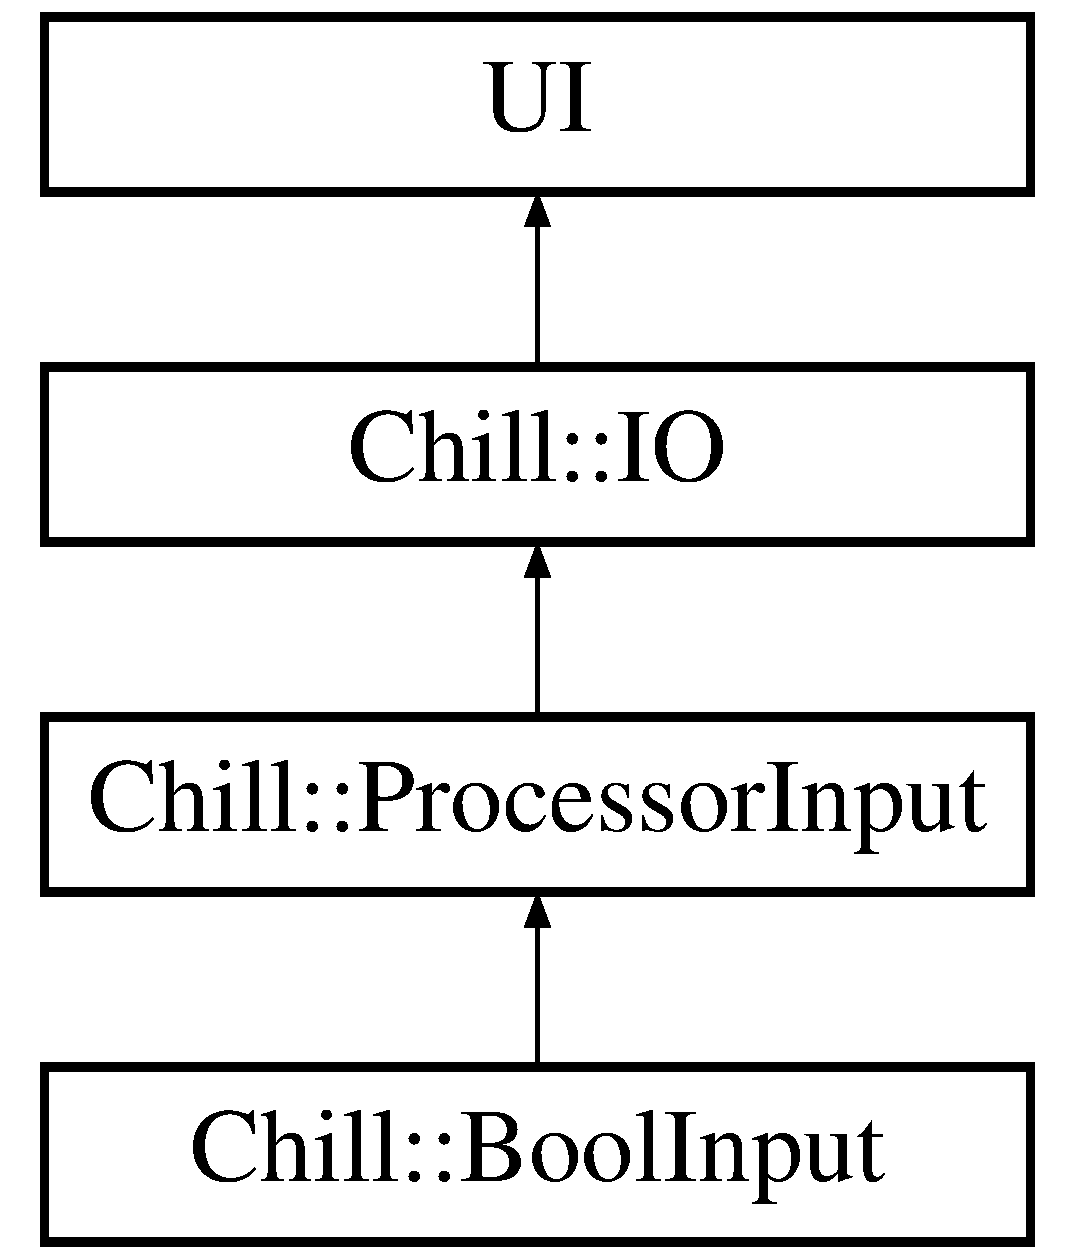
\includegraphics[height=4.000000cm]{class_chill_1_1_bool_input}
\end{center}
\end{figure}
\subsection*{Public Member Functions}
\begin{DoxyCompactItemize}
\item 
\mbox{\Hypertarget{class_chill_1_1_bool_input_aae2e8cc8286c1bc2e1a86d2a1df1b8e3}\label{class_chill_1_1_bool_input_aae2e8cc8286c1bc2e1a86d2a1df1b8e3}} 
{\footnotesize template$<$typename ... Args$>$ }\\{\bfseries Bool\+Input} (bool \+\_\+value=false, Args \&\&...)
\item 
\mbox{\Hypertarget{class_chill_1_1_bool_input_a3fbc0d1f7a014f66a3e2694e9a504a9a}\label{class_chill_1_1_bool_input_a3fbc0d1f7a014f66a3e2694e9a504a9a}} 
bool {\bfseries draw\+Tweak} ()
\item 
\mbox{\Hypertarget{class_chill_1_1_bool_input_a476fbe3663b4dd60bbc212ab64aeb4b5}\label{class_chill_1_1_bool_input_a476fbe3663b4dd60bbc212ab64aeb4b5}} 
Auto\+Ptr$<$ \mbox{\hyperlink{class_chill_1_1_processor_input}{Processor\+Input}} $>$ {\bfseries clone} ()
\item 
\mbox{\Hypertarget{class_chill_1_1_bool_input_ad8c8c597733d4d53a38005fa852090e4}\label{class_chill_1_1_bool_input_ad8c8c597733d4d53a38005fa852090e4}} 
void {\bfseries save} (std\+::ofstream \&\+\_\+stream)
\end{DoxyCompactItemize}
\subsection*{Public Attributes}
\begin{DoxyCompactItemize}
\item 
\mbox{\Hypertarget{class_chill_1_1_bool_input_a2942d4164fe50893e591a3799db34dc5}\label{class_chill_1_1_bool_input_a2942d4164fe50893e591a3799db34dc5}} 
bool {\bfseries m\+\_\+value}
\end{DoxyCompactItemize}
\subsection*{Additional Inherited Members}


The documentation for this class was generated from the following files\+:\begin{DoxyCompactItemize}
\item 
E\+:/\+Chill/chill/chill\+Engine/\mbox{\hyperlink{_i_os_8h}{I\+Os.\+h}}\item 
E\+:/\+Chill/chill/chill\+Engine/I\+Os.\+cpp\end{DoxyCompactItemize}

\hypertarget{class_chill_1_1_bool_output}{}\section{Chill\+:\+:Bool\+Output Class Reference}
\label{class_chill_1_1_bool_output}\index{Chill\+::\+Bool\+Output@{Chill\+::\+Bool\+Output}}
Inheritance diagram for Chill\+:\+:Bool\+Output\+:\begin{figure}[H]
\begin{center}
\leavevmode
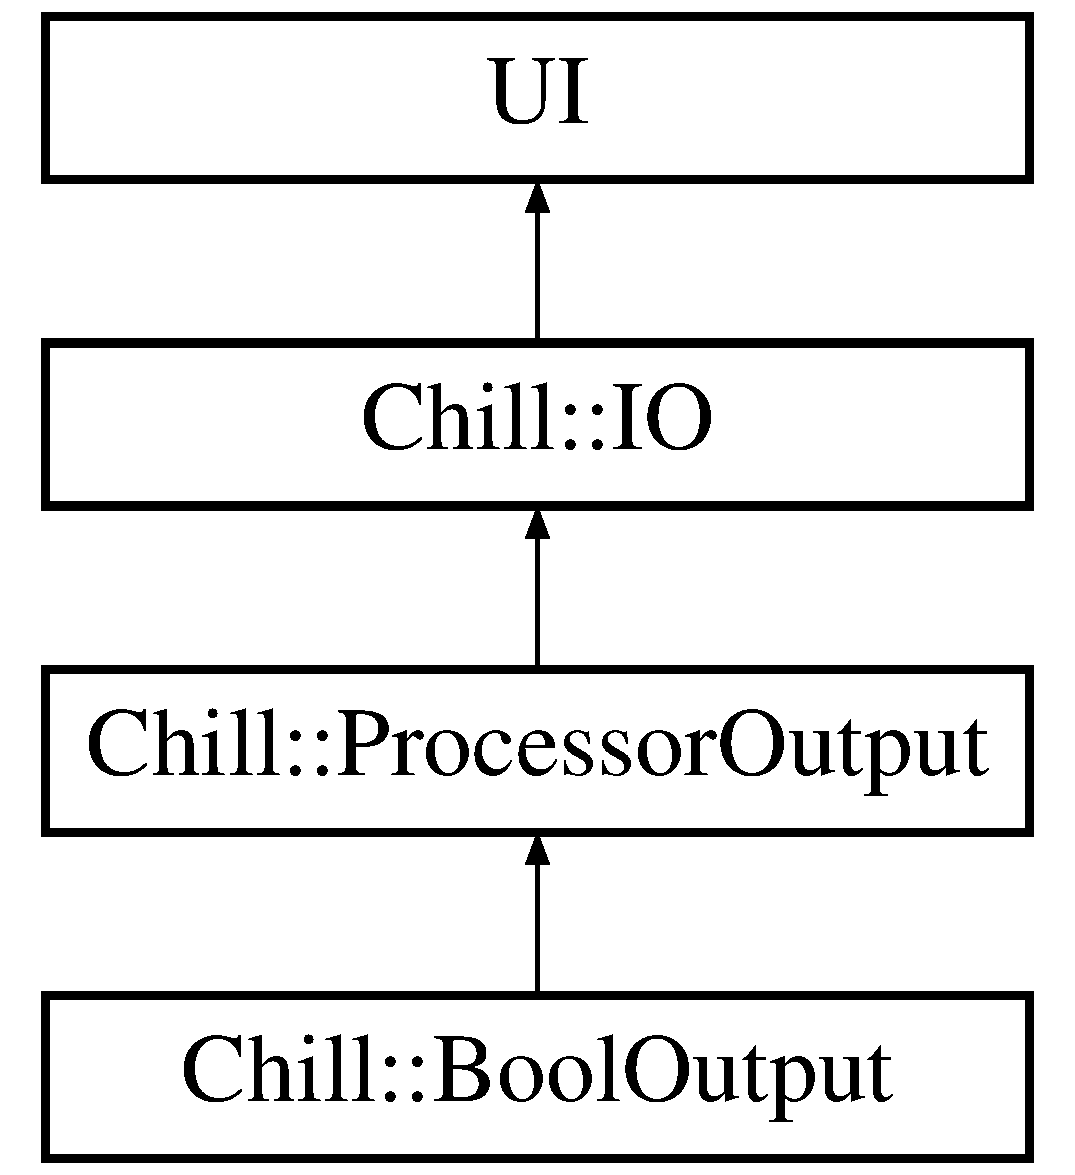
\includegraphics[height=4.000000cm]{class_chill_1_1_bool_output}
\end{center}
\end{figure}
\subsection*{Public Member Functions}
\begin{DoxyCompactItemize}
\item 
\mbox{\Hypertarget{class_chill_1_1_bool_output_a58f478050c8bda9d743085f69ccaa8d7}\label{class_chill_1_1_bool_output_a58f478050c8bda9d743085f69ccaa8d7}} 
Auto\+Ptr$<$ \mbox{\hyperlink{class_chill_1_1_processor_output}{Processor\+Output}} $>$ {\bfseries clone} ()
\end{DoxyCompactItemize}
\subsection*{Additional Inherited Members}


The documentation for this class was generated from the following file\+:\begin{DoxyCompactItemize}
\item 
E\+:/\+Chill/chill/chill\+Engine/\mbox{\hyperlink{_i_os_8h}{I\+Os.\+h}}\end{DoxyCompactItemize}

\hypertarget{class_chill_1_1_graph_saver}{}\section{Chill\+:\+:Graph\+Saver Class Reference}
\label{class_chill_1_1_graph_saver}\index{Chill\+::\+Graph\+Saver@{Chill\+::\+Graph\+Saver}}
\subsection*{Public Member Functions}
\begin{DoxyCompactItemize}
\item 
\mbox{\Hypertarget{class_chill_1_1_graph_saver_a7a756b52e41c7df7057f138781800859}\label{class_chill_1_1_graph_saver_a7a756b52e41c7df7057f138781800859}} 
void {\bfseries execute} (const char $\ast$\+\_\+path)
\item 
\mbox{\Hypertarget{class_chill_1_1_graph_saver_aad11a2eab9b5d2a313e6435a18bb1069}\label{class_chill_1_1_graph_saver_aad11a2eab9b5d2a313e6435a18bb1069}} 
void {\bfseries register\+Bindings} (lua\+\_\+\+State $\ast$\+\_\+L)
\end{DoxyCompactItemize}


The documentation for this class was generated from the following files\+:\begin{DoxyCompactItemize}
\item 
E\+:/\+Chill/chill/chill\+Engine/Graph\+Saver.\+h\item 
E\+:/\+Chill/chill/chill\+Engine/Graph\+Saver.\+cpp\end{DoxyCompactItemize}

\hypertarget{class_chill_1_1_group_processor}{}\section{Chill\+:\+:Group\+Processor Class Reference}
\label{class_chill_1_1_group_processor}\index{Chill\+::\+Group\+Processor@{Chill\+::\+Group\+Processor}}
Inheritance diagram for Chill\+:\+:Group\+Processor\+:\begin{figure}[H]
\begin{center}
\leavevmode
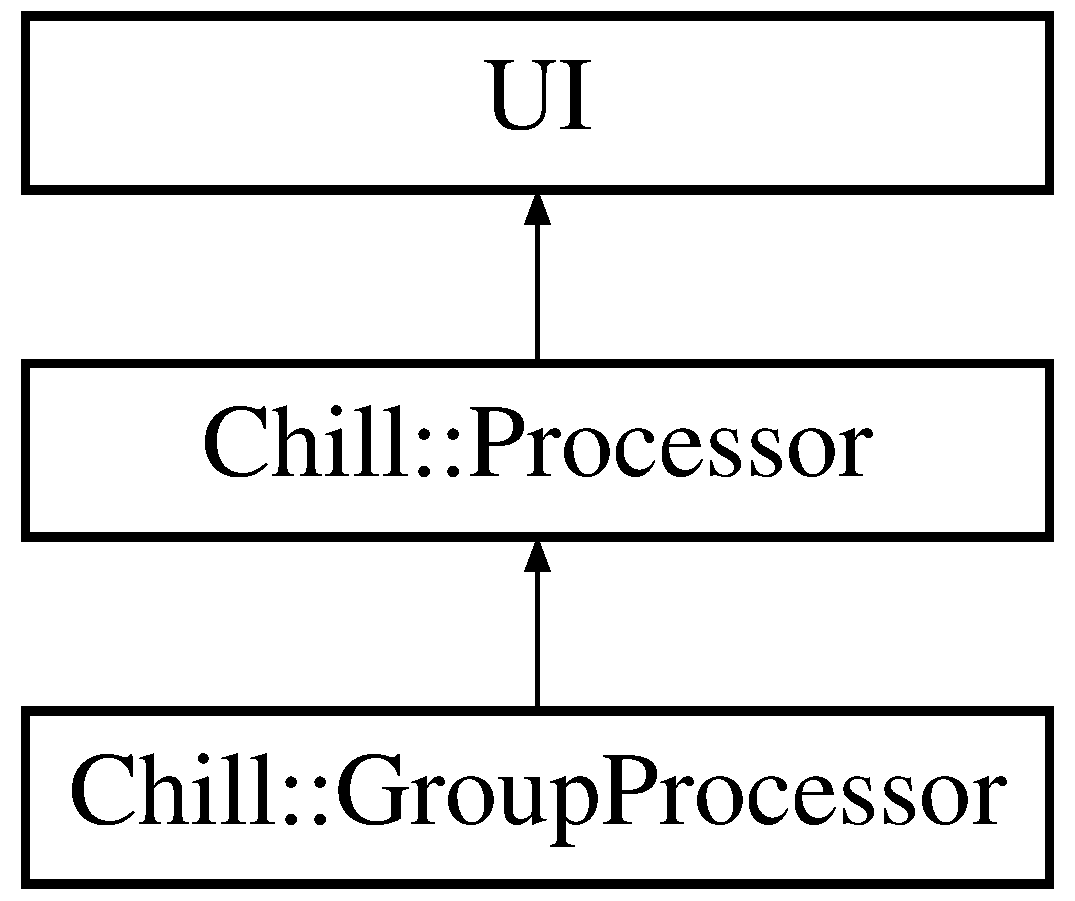
\includegraphics[height=3.000000cm]{class_chill_1_1_group_processor}
\end{center}
\end{figure}
\subsection*{Public Member Functions}
\begin{DoxyCompactItemize}
\item 
\mbox{\Hypertarget{class_chill_1_1_group_processor_a3d24966d2aa972cdceed46832c585039}\label{class_chill_1_1_group_processor_a3d24966d2aa972cdceed46832c585039}} 
virtual Auto\+Ptr$<$ \mbox{\hyperlink{class_chill_1_1_processor}{Processor}} $>$ {\bfseries clone} () override
\item 
virtual bool \mbox{\hyperlink{class_chill_1_1_group_processor_a6c3eadfcb171c48a2d76bebefd153fcb}{draw}} ()
\item 
\mbox{\Hypertarget{class_chill_1_1_group_processor_ab87cb5cbe1d8d41d3c85c93d57024ba9}\label{class_chill_1_1_group_processor_ab87cb5cbe1d8d41d3c85c93d57024ba9}} 
void {\bfseries set\+Input\+Mode} (bool mode\+\_\+)
\item 
\mbox{\Hypertarget{class_chill_1_1_group_processor_a009f7866148cf7ed3c0957139bedded5}\label{class_chill_1_1_group_processor_a009f7866148cf7ed3c0957139bedded5}} 
void {\bfseries set\+Output\+Mode} (bool mode\+\_\+)
\end{DoxyCompactItemize}
\subsection*{Additional Inherited Members}


\subsection{Member Function Documentation}
\mbox{\Hypertarget{class_chill_1_1_group_processor_a6c3eadfcb171c48a2d76bebefd153fcb}\label{class_chill_1_1_group_processor_a6c3eadfcb171c48a2d76bebefd153fcb}} 
\index{Chill\+::\+Group\+Processor@{Chill\+::\+Group\+Processor}!draw@{draw}}
\index{draw@{draw}!Chill\+::\+Group\+Processor@{Chill\+::\+Group\+Processor}}
\subsubsection{\texorpdfstring{draw()}{draw()}}
{\footnotesize\ttfamily bool Chill\+::\+Group\+Processor\+::draw (\begin{DoxyParamCaption}{ }\end{DoxyParamCaption})\hspace{0.3cm}{\ttfamily [virtual]}}

Draw the processor 

Reimplemented from \mbox{\hyperlink{class_chill_1_1_processor_a2eb86d9750e1c0d5ac7f6da166aca8fd}{Chill\+::\+Processor}}.



The documentation for this class was generated from the following files\+:\begin{DoxyCompactItemize}
\item 
E\+:/\+Chill/chill/chill\+Engine/\mbox{\hyperlink{_processor_8h}{Processor.\+h}}\item 
E\+:/\+Chill/chill/chill\+Engine/Group\+Processors.\+cpp\end{DoxyCompactItemize}

\hypertarget{class_chill_1_1_int_input}{}\section{Chill\+:\+:Int\+Input Class Reference}
\label{class_chill_1_1_int_input}\index{Chill\+::\+Int\+Input@{Chill\+::\+Int\+Input}}
Inheritance diagram for Chill\+:\+:Int\+Input\+:\begin{figure}[H]
\begin{center}
\leavevmode
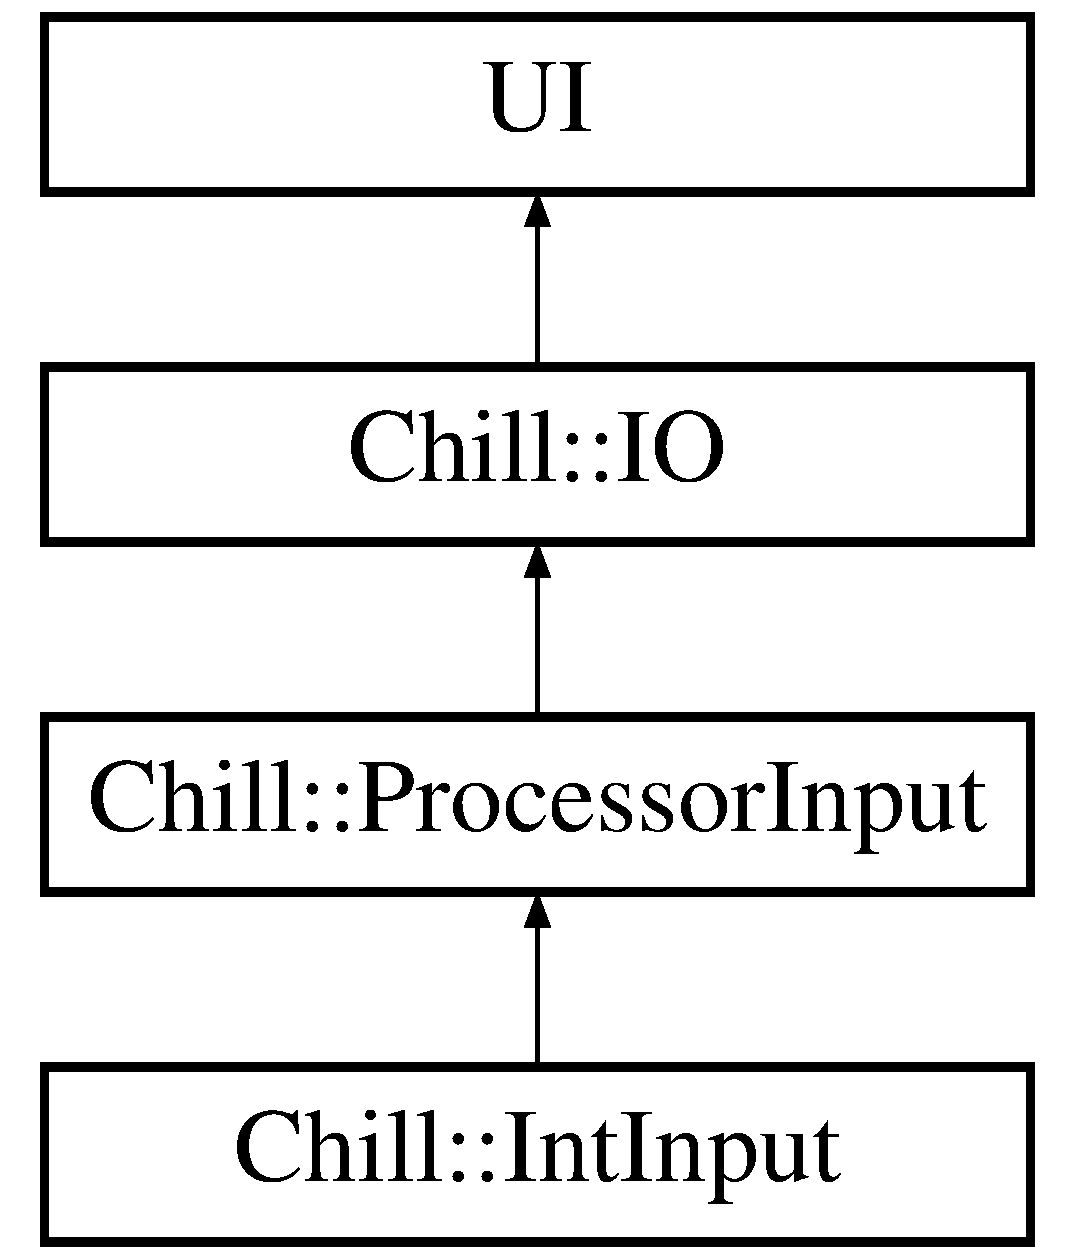
\includegraphics[height=4.000000cm]{class_chill_1_1_int_input}
\end{center}
\end{figure}
\subsection*{Public Member Functions}
\begin{DoxyCompactItemize}
\item 
\mbox{\Hypertarget{class_chill_1_1_int_input_a1103252b1a63f9f4b0b44e92846384aa}\label{class_chill_1_1_int_input_a1103252b1a63f9f4b0b44e92846384aa}} 
{\footnotesize template$<$typename ... Args$>$ }\\{\bfseries Int\+Input} (float $\ast$\+\_\+values, Args \&\&... \+\_\+args)
\item 
\mbox{\Hypertarget{class_chill_1_1_int_input_a773428cabf7d5948bd328d1f5da5b741}\label{class_chill_1_1_int_input_a773428cabf7d5948bd328d1f5da5b741}} 
{\footnotesize template$<$typename ... Args$>$ }\\{\bfseries Int\+Input} (int \+\_\+value=0, int \+\_\+min=min(), int \+\_\+max=max(), bool \+\_\+slider=false, int \+\_\+step=step(), Args \&\&...)
\item 
\mbox{\Hypertarget{class_chill_1_1_int_input_a70f972bfe906bc86340b60739a788e49}\label{class_chill_1_1_int_input_a70f972bfe906bc86340b60739a788e49}} 
bool {\bfseries draw\+Tweak} ()
\item 
\mbox{\Hypertarget{class_chill_1_1_int_input_a8be2de3ae3ce511d433aab4cbd228ccb}\label{class_chill_1_1_int_input_a8be2de3ae3ce511d433aab4cbd228ccb}} 
Auto\+Ptr$<$ \mbox{\hyperlink{class_chill_1_1_processor_input}{Processor\+Input}} $>$ {\bfseries clone} ()
\item 
\mbox{\Hypertarget{class_chill_1_1_int_input_a260a4ede837d1d025381aac5b1bc3a18}\label{class_chill_1_1_int_input_a260a4ede837d1d025381aac5b1bc3a18}} 
void {\bfseries save} (std\+::ofstream \&\+\_\+stream)
\end{DoxyCompactItemize}
\subsection*{Static Public Member Functions}
\begin{DoxyCompactItemize}
\item 
\mbox{\Hypertarget{class_chill_1_1_int_input_a61f8051dcbc2bf06e5a6e9ea86580fa1}\label{class_chill_1_1_int_input_a61f8051dcbc2bf06e5a6e9ea86580fa1}} 
static int {\bfseries min} ()
\item 
\mbox{\Hypertarget{class_chill_1_1_int_input_a8a26e5b95b8446fcbe4027d0f81eb900}\label{class_chill_1_1_int_input_a8a26e5b95b8446fcbe4027d0f81eb900}} 
static int {\bfseries max} ()
\item 
\mbox{\Hypertarget{class_chill_1_1_int_input_ad34cb8c956737458505350fee8fb9929}\label{class_chill_1_1_int_input_ad34cb8c956737458505350fee8fb9929}} 
static int {\bfseries step} ()
\end{DoxyCompactItemize}
\subsection*{Public Attributes}
\begin{DoxyCompactItemize}
\item 
\mbox{\Hypertarget{class_chill_1_1_int_input_ac478c9f2f7c637f74e0cb285ffd9a48a}\label{class_chill_1_1_int_input_ac478c9f2f7c637f74e0cb285ffd9a48a}} 
int {\bfseries m\+\_\+value}
\item 
\mbox{\Hypertarget{class_chill_1_1_int_input_aad053b1d19511506c50d5b23b48b0621}\label{class_chill_1_1_int_input_aad053b1d19511506c50d5b23b48b0621}} 
int {\bfseries m\+\_\+min}
\item 
\mbox{\Hypertarget{class_chill_1_1_int_input_aa3e4ca0362c622ce7fab831404137670}\label{class_chill_1_1_int_input_aa3e4ca0362c622ce7fab831404137670}} 
int {\bfseries m\+\_\+max}
\item 
\mbox{\Hypertarget{class_chill_1_1_int_input_a2229ad2116d497f8b1bf110e1598774e}\label{class_chill_1_1_int_input_a2229ad2116d497f8b1bf110e1598774e}} 
bool {\bfseries m\+\_\+slider}
\item 
\mbox{\Hypertarget{class_chill_1_1_int_input_aa12824fbe3a4083906ccde9b7c097944}\label{class_chill_1_1_int_input_aa12824fbe3a4083906ccde9b7c097944}} 
int {\bfseries m\+\_\+step}
\end{DoxyCompactItemize}


The documentation for this class was generated from the following files\+:\begin{DoxyCompactItemize}
\item 
E\+:/\+Chill/chill/chill\+Engine/\mbox{\hyperlink{_i_os_8h}{I\+Os.\+h}}\item 
E\+:/\+Chill/chill/chill\+Engine/I\+Os.\+cpp\end{DoxyCompactItemize}

\hypertarget{class_chill_1_1_int_output}{}\section{Chill\+:\+:Int\+Output Class Reference}
\label{class_chill_1_1_int_output}\index{Chill\+::\+Int\+Output@{Chill\+::\+Int\+Output}}
Inheritance diagram for Chill\+:\+:Int\+Output\+:\begin{figure}[H]
\begin{center}
\leavevmode
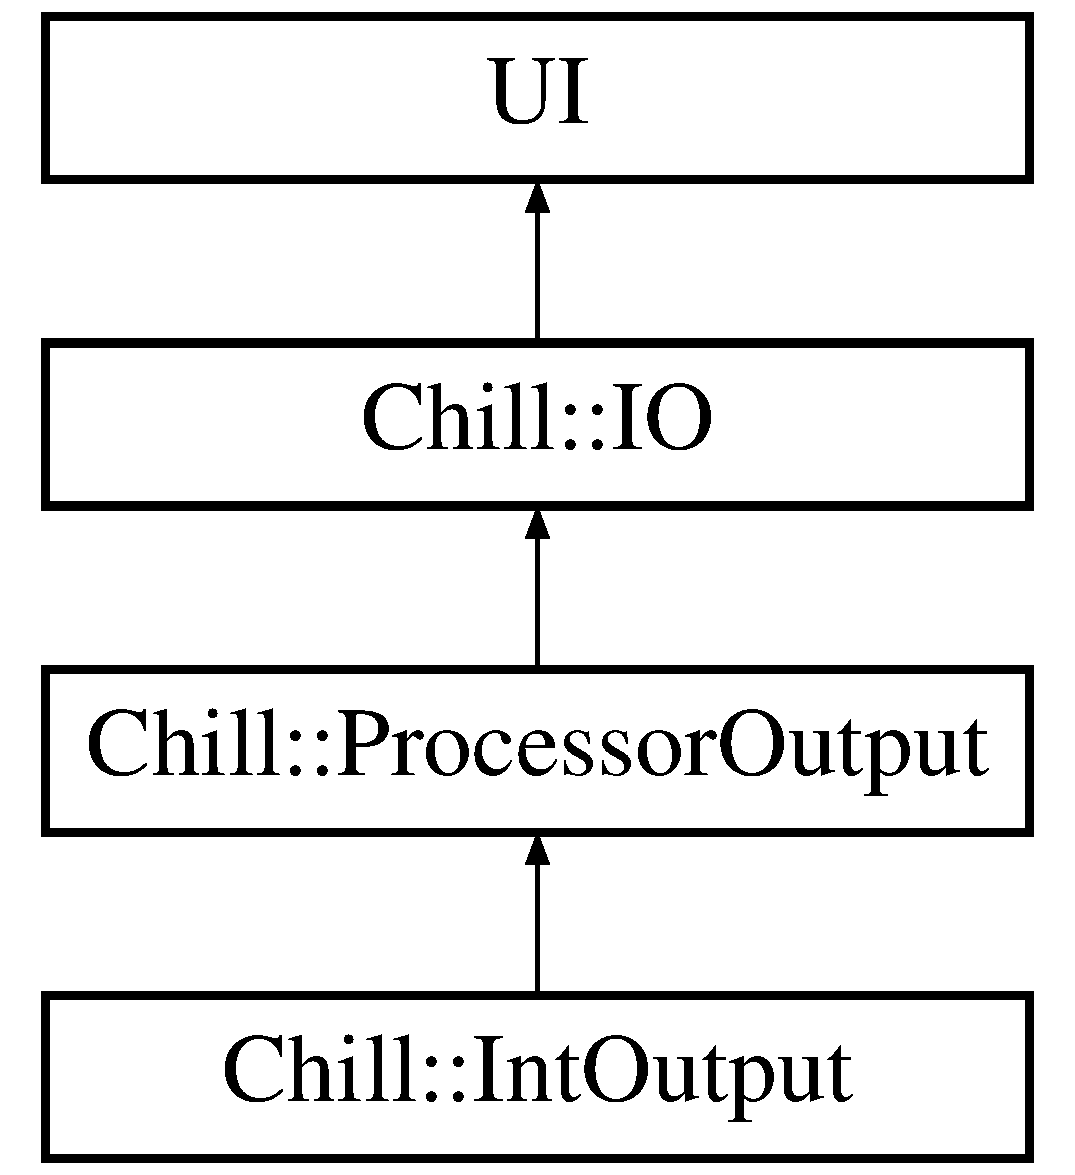
\includegraphics[height=4.000000cm]{class_chill_1_1_int_output}
\end{center}
\end{figure}
\subsection*{Public Member Functions}
\begin{DoxyCompactItemize}
\item 
\mbox{\Hypertarget{class_chill_1_1_int_output_a40398ba114010bc4d7f585f4da8cddd9}\label{class_chill_1_1_int_output_a40398ba114010bc4d7f585f4da8cddd9}} 
Auto\+Ptr$<$ \mbox{\hyperlink{class_chill_1_1_processor_output}{Processor\+Output}} $>$ {\bfseries clone} ()
\end{DoxyCompactItemize}
\subsection*{Additional Inherited Members}


The documentation for this class was generated from the following file\+:\begin{DoxyCompactItemize}
\item 
E\+:/\+Chill/chill/chill\+Engine/\mbox{\hyperlink{_i_os_8h}{I\+Os.\+h}}\end{DoxyCompactItemize}

\hypertarget{class_chill_1_1_i_o}{}\section{Chill\+:\+:IO Class Reference}
\label{class_chill_1_1_i_o}\index{Chill\+::\+IO@{Chill\+::\+IO}}
Inheritance diagram for Chill\+:\+:IO\+:\begin{figure}[H]
\begin{center}
\leavevmode
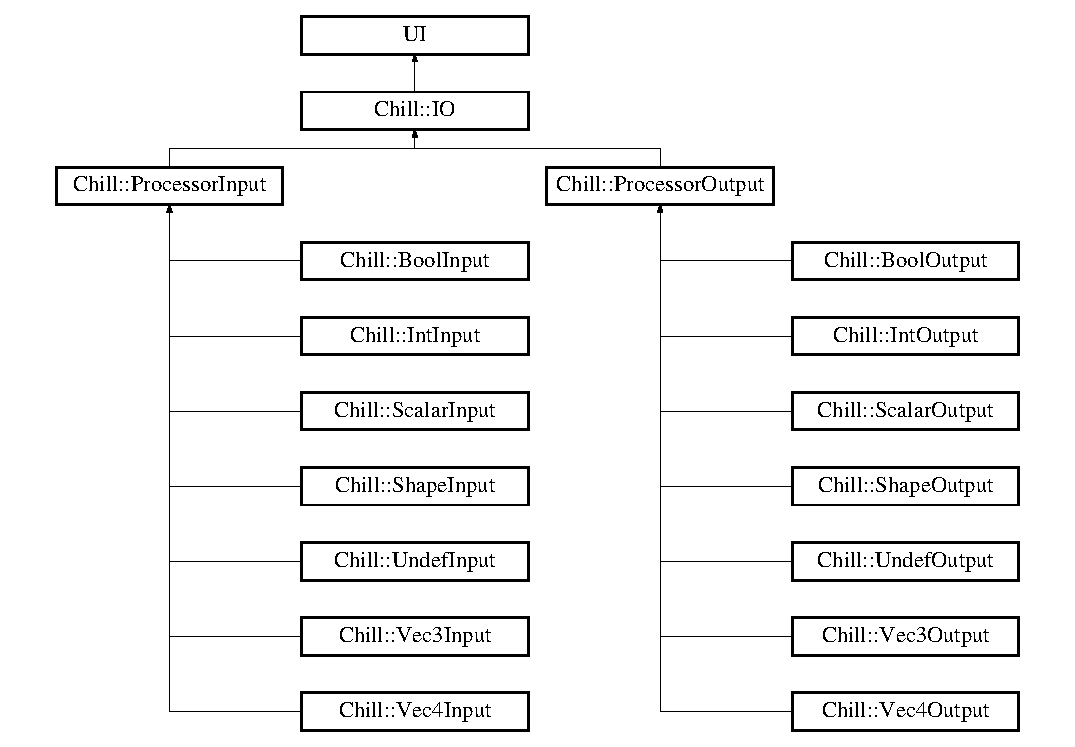
\includegraphics[height=9.589041cm]{class_chill_1_1_i_o}
\end{center}
\end{figure}
\subsection*{Public Member Functions}
\begin{DoxyCompactItemize}
\item 
\mbox{\Hypertarget{class_chill_1_1_i_o_ac639842a6d9bfa75a8aecfef6887b6f1}\label{class_chill_1_1_i_o_ac639842a6d9bfa75a8aecfef6887b6f1}} 
\mbox{\hyperlink{class_chill_1_1_processor}{Processor}} $\ast$ {\bfseries owner} ()
\item 
\mbox{\Hypertarget{class_chill_1_1_i_o_ad3fc42bb1940d0ca734ec516775cd0fd}\label{class_chill_1_1_i_o_ad3fc42bb1940d0ca734ec516775cd0fd}} 
const char $\ast$ {\bfseries name} ()
\item 
\mbox{\Hypertarget{class_chill_1_1_i_o_a9cb1a5df93ba477db683f0a4506d7926}\label{class_chill_1_1_i_o_a9cb1a5df93ba477db683f0a4506d7926}} 
const I\+O\+Type\+::\+I\+O\+Type {\bfseries type} ()
\end{DoxyCompactItemize}
\subsection*{Public Attributes}
\begin{DoxyCompactItemize}
\item 
\mbox{\hyperlink{class_chill_1_1_processor}{Processor}} $\ast$ \mbox{\hyperlink{class_chill_1_1_i_o_a88eff91ac0f77cf4c9d307615452f365}{m\+\_\+owner}}
\item 
I\+O\+Type\+::\+I\+O\+Type \mbox{\hyperlink{class_chill_1_1_i_o_adc235c7126e87e8af02631b5b9a94b0a}{m\+\_\+type}}
\item 
std\+::string \mbox{\hyperlink{class_chill_1_1_i_o_a1f41050855e77ca7aeb97fff0c59f59a}{m\+\_\+name}}
\item 
Im\+U32 \mbox{\hyperlink{class_chill_1_1_i_o_a1bba12c357581b8b61c2bde579f4078b}{m\+\_\+color}}
\end{DoxyCompactItemize}


\subsection{Member Data Documentation}
\mbox{\Hypertarget{class_chill_1_1_i_o_a1bba12c357581b8b61c2bde579f4078b}\label{class_chill_1_1_i_o_a1bba12c357581b8b61c2bde579f4078b}} 
\index{Chill\+::\+IO@{Chill\+::\+IO}!m\+\_\+color@{m\+\_\+color}}
\index{m\+\_\+color@{m\+\_\+color}!Chill\+::\+IO@{Chill\+::\+IO}}
\subsubsection{\texorpdfstring{m\+\_\+color}{m\_color}}
{\footnotesize\ttfamily Im\+U32 Chill\+::\+I\+O\+::m\+\_\+color}

Display color. \mbox{\Hypertarget{class_chill_1_1_i_o_a1f41050855e77ca7aeb97fff0c59f59a}\label{class_chill_1_1_i_o_a1f41050855e77ca7aeb97fff0c59f59a}} 
\index{Chill\+::\+IO@{Chill\+::\+IO}!m\+\_\+name@{m\+\_\+name}}
\index{m\+\_\+name@{m\+\_\+name}!Chill\+::\+IO@{Chill\+::\+IO}}
\subsubsection{\texorpdfstring{m\+\_\+name}{m\_name}}
{\footnotesize\ttfamily std\+::string Chill\+::\+I\+O\+::m\+\_\+name}

Display name. \mbox{\Hypertarget{class_chill_1_1_i_o_a88eff91ac0f77cf4c9d307615452f365}\label{class_chill_1_1_i_o_a88eff91ac0f77cf4c9d307615452f365}} 
\index{Chill\+::\+IO@{Chill\+::\+IO}!m\+\_\+owner@{m\+\_\+owner}}
\index{m\+\_\+owner@{m\+\_\+owner}!Chill\+::\+IO@{Chill\+::\+IO}}
\subsubsection{\texorpdfstring{m\+\_\+owner}{m\_owner}}
{\footnotesize\ttfamily \mbox{\hyperlink{class_chill_1_1_processor}{Processor}}$\ast$ Chill\+::\+I\+O\+::m\+\_\+owner}

Parent processor, raw pointer is needed. \mbox{\Hypertarget{class_chill_1_1_i_o_adc235c7126e87e8af02631b5b9a94b0a}\label{class_chill_1_1_i_o_adc235c7126e87e8af02631b5b9a94b0a}} 
\index{Chill\+::\+IO@{Chill\+::\+IO}!m\+\_\+type@{m\+\_\+type}}
\index{m\+\_\+type@{m\+\_\+type}!Chill\+::\+IO@{Chill\+::\+IO}}
\subsubsection{\texorpdfstring{m\+\_\+type}{m\_type}}
{\footnotesize\ttfamily I\+O\+Type\+::\+I\+O\+Type Chill\+::\+I\+O\+::m\+\_\+type}

Expected data type. 

The documentation for this class was generated from the following file\+:\begin{DoxyCompactItemize}
\item 
E\+:/\+Chill/chill/chill\+Engine/\mbox{\hyperlink{_i_os_8h}{I\+Os.\+h}}\end{DoxyCompactItemize}

\hypertarget{class_chill_1_1_lua___graph}{}\section{Chill\+:\+:Lua\+\_\+\+Graph Class Reference}
\label{class_chill_1_1_lua___graph}\index{Chill\+::\+Lua\+\_\+\+Graph@{Chill\+::\+Lua\+\_\+\+Graph}}
Inheritance diagram for Chill\+:\+:Lua\+\_\+\+Graph\+:\begin{figure}[H]
\begin{center}
\leavevmode
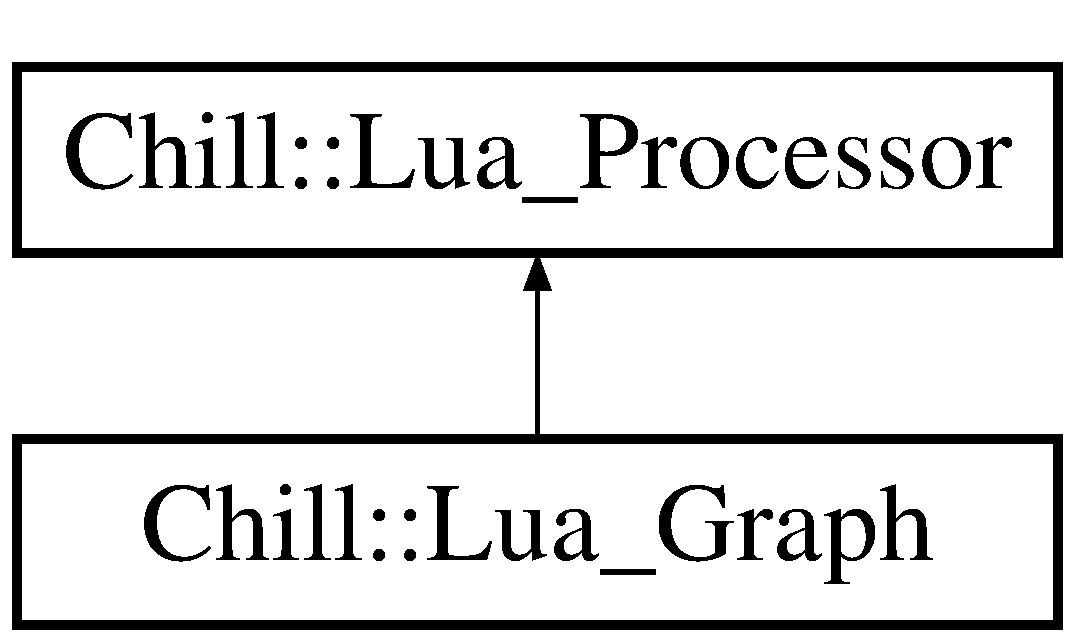
\includegraphics[height=2.000000cm]{class_chill_1_1_lua___graph}
\end{center}
\end{figure}
\subsection*{Public Member Functions}
\begin{DoxyCompactItemize}
\item 
\mbox{\Hypertarget{class_chill_1_1_lua___graph_a9c6f01507d4ea76b9f5cf0cb6e7cd3e6}\label{class_chill_1_1_lua___graph_a9c6f01507d4ea76b9f5cf0cb6e7cd3e6}} 
{\bfseries Lua\+\_\+\+Graph} (const std\+::string \&name\+\_\+)
\item 
\mbox{\Hypertarget{class_chill_1_1_lua___graph_a47fa0453dab0cb95842374ddf9da1661}\label{class_chill_1_1_lua___graph_a47fa0453dab0cb95842374ddf9da1661}} 
{\bfseries Lua\+\_\+\+Graph} (const object \&table)
\item 
\mbox{\Hypertarget{class_chill_1_1_lua___graph_adef0f02440498754dc11efa2e3318d84}\label{class_chill_1_1_lua___graph_adef0f02440498754dc11efa2e3318d84}} 
void {\bfseries add\+Processor} (\mbox{\hyperlink{class_chill_1_1_lua___processor}{Lua\+\_\+\+Processor}} \&proc)
\end{DoxyCompactItemize}
\subsection*{Additional Inherited Members}


The documentation for this class was generated from the following file\+:\begin{DoxyCompactItemize}
\item 
E\+:/\+Chill/chill/chill\+Engine/Graph\+Saver.\+cpp\end{DoxyCompactItemize}

\hypertarget{class_chill_1_1_lua___input}{}\section{Chill\+:\+:Lua\+\_\+\+Input Class Reference}
\label{class_chill_1_1_lua___input}\index{Chill\+::\+Lua\+\_\+\+Input@{Chill\+::\+Lua\+\_\+\+Input}}
\subsection*{Public Member Functions}
\begin{DoxyCompactItemize}
\item 
\mbox{\Hypertarget{class_chill_1_1_lua___input_aebbfcc46776a36fd960ee0bf974342c0}\label{class_chill_1_1_lua___input_aebbfcc46776a36fd960ee0bf974342c0}} 
{\bfseries Lua\+\_\+\+Input} (const object \&table)
\item 
\mbox{\Hypertarget{class_chill_1_1_lua___input_a36deda5e1529c5e8cc5e3de94b0f900a}\label{class_chill_1_1_lua___input_a36deda5e1529c5e8cc5e3de94b0f900a}} 
Auto\+Ptr$<$ \mbox{\hyperlink{class_chill_1_1_processor_input}{Processor\+Input}} $>$ \& {\bfseries ptr} ()
\end{DoxyCompactItemize}
\subsection*{Protected Attributes}
\begin{DoxyCompactItemize}
\item 
\mbox{\Hypertarget{class_chill_1_1_lua___input_a42c13f028f1a8eb593eee9537e932493}\label{class_chill_1_1_lua___input_a42c13f028f1a8eb593eee9537e932493}} 
Auto\+Ptr$<$ \mbox{\hyperlink{class_chill_1_1_processor_input}{Processor\+Input}} $>$ {\bfseries m\+\_\+\+Ptr}
\end{DoxyCompactItemize}


The documentation for this class was generated from the following file\+:\begin{DoxyCompactItemize}
\item 
E\+:/\+Chill/chill/chill\+Engine/Graph\+Saver.\+cpp\end{DoxyCompactItemize}

\hypertarget{class_chill_1_1_lua___node}{}\section{Chill\+:\+:Lua\+\_\+\+Node Class Reference}
\label{class_chill_1_1_lua___node}\index{Chill\+::\+Lua\+\_\+\+Node@{Chill\+::\+Lua\+\_\+\+Node}}
Inheritance diagram for Chill\+:\+:Lua\+\_\+\+Node\+:\begin{figure}[H]
\begin{center}
\leavevmode
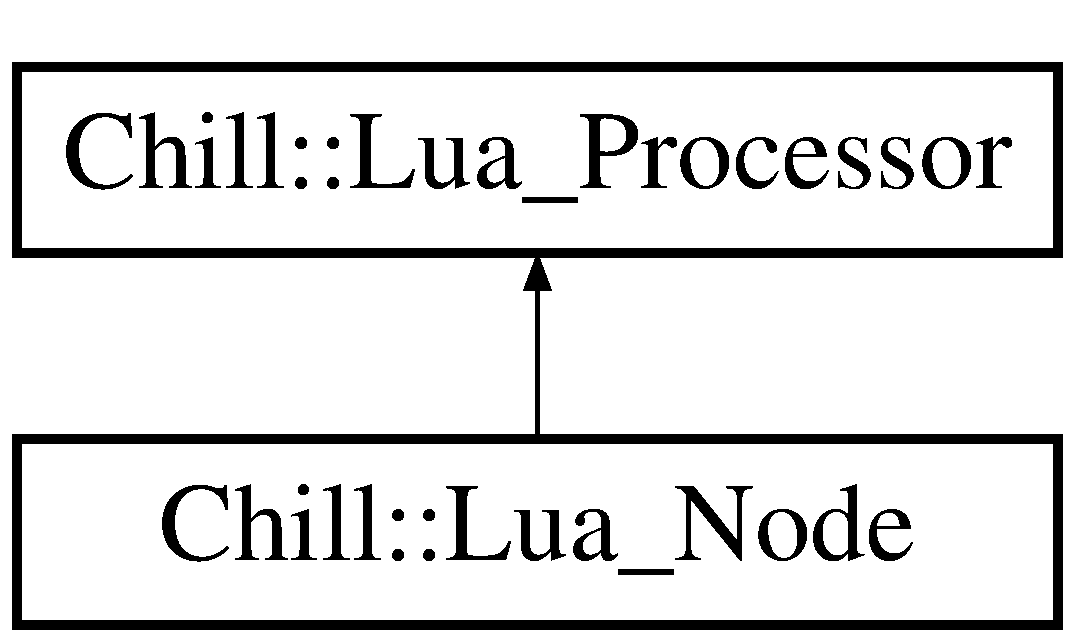
\includegraphics[height=2.000000cm]{class_chill_1_1_lua___node}
\end{center}
\end{figure}
\subsection*{Public Member Functions}
\begin{DoxyCompactItemize}
\item 
\mbox{\Hypertarget{class_chill_1_1_lua___node_afccc165b818a958f872590c5294d613a}\label{class_chill_1_1_lua___node_afccc165b818a958f872590c5294d613a}} 
{\bfseries Lua\+\_\+\+Node} (const std\+::string \&name\+\_\+)
\item 
\mbox{\Hypertarget{class_chill_1_1_lua___node_ac890079e18a78070435fa9eb76f6d4ad}\label{class_chill_1_1_lua___node_ac890079e18a78070435fa9eb76f6d4ad}} 
{\bfseries Lua\+\_\+\+Node} (const object \&table)
\end{DoxyCompactItemize}
\subsection*{Additional Inherited Members}


The documentation for this class was generated from the following file\+:\begin{DoxyCompactItemize}
\item 
E\+:/\+Chill/chill/chill\+Engine/Graph\+Saver.\+cpp\end{DoxyCompactItemize}

\hypertarget{class_chill_1_1_lua___output}{}\section{Chill\+:\+:Lua\+\_\+\+Output Class Reference}
\label{class_chill_1_1_lua___output}\index{Chill\+::\+Lua\+\_\+\+Output@{Chill\+::\+Lua\+\_\+\+Output}}
\subsection*{Public Member Functions}
\begin{DoxyCompactItemize}
\item 
\mbox{\Hypertarget{class_chill_1_1_lua___output_a464b74e7af8cb34b82d4f73666b90ab4}\label{class_chill_1_1_lua___output_a464b74e7af8cb34b82d4f73666b90ab4}} 
{\bfseries Lua\+\_\+\+Output} (const object \&table)
\item 
\mbox{\Hypertarget{class_chill_1_1_lua___output_a6428a65075b6a5430735829b9e4bcd82}\label{class_chill_1_1_lua___output_a6428a65075b6a5430735829b9e4bcd82}} 
Auto\+Ptr$<$ \mbox{\hyperlink{class_chill_1_1_processor_output}{Processor\+Output}} $>$ \& {\bfseries ptr} ()
\end{DoxyCompactItemize}
\subsection*{Protected Attributes}
\begin{DoxyCompactItemize}
\item 
\mbox{\Hypertarget{class_chill_1_1_lua___output_a4cf36639153e56c48c3b4e855fa3d65a}\label{class_chill_1_1_lua___output_a4cf36639153e56c48c3b4e855fa3d65a}} 
Auto\+Ptr$<$ \mbox{\hyperlink{class_chill_1_1_processor_output}{Processor\+Output}} $>$ {\bfseries m\+\_\+\+Ptr}
\end{DoxyCompactItemize}


The documentation for this class was generated from the following file\+:\begin{DoxyCompactItemize}
\item 
E\+:/\+Chill/chill/chill\+Engine/Graph\+Saver.\+cpp\end{DoxyCompactItemize}

\hypertarget{class_chill_1_1_lua___processor}{}\section{Chill\+:\+:Lua\+\_\+\+Processor Class Reference}
\label{class_chill_1_1_lua___processor}\index{Chill\+::\+Lua\+\_\+\+Processor@{Chill\+::\+Lua\+\_\+\+Processor}}
Inheritance diagram for Chill\+:\+:Lua\+\_\+\+Processor\+:\begin{figure}[H]
\begin{center}
\leavevmode
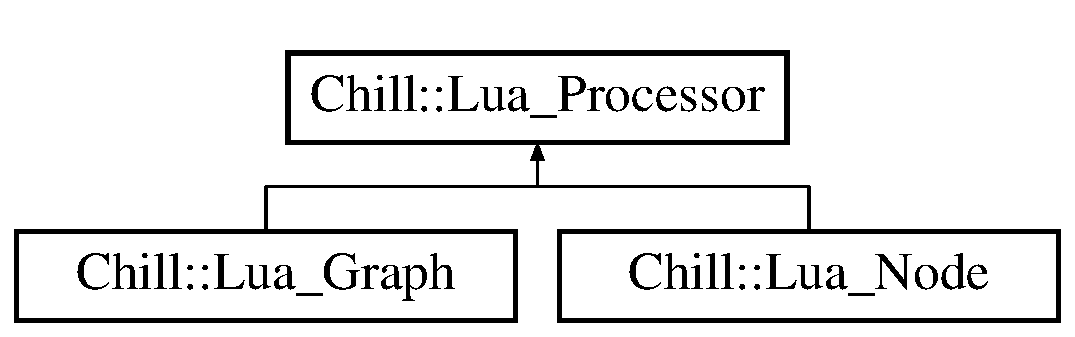
\includegraphics[height=2.000000cm]{class_chill_1_1_lua___processor}
\end{center}
\end{figure}
\subsection*{Public Member Functions}
\begin{DoxyCompactItemize}
\item 
\mbox{\Hypertarget{class_chill_1_1_lua___processor_a01aeb9acab82db2c119ae71ed5208d13}\label{class_chill_1_1_lua___processor_a01aeb9acab82db2c119ae71ed5208d13}} 
{\bfseries Lua\+\_\+\+Processor} (const std\+::string \&name\+\_\+)
\item 
\mbox{\Hypertarget{class_chill_1_1_lua___processor_a62874754d5193c80b899ce0d10f50a70}\label{class_chill_1_1_lua___processor_a62874754d5193c80b899ce0d10f50a70}} 
{\bfseries Lua\+\_\+\+Processor} (const object \&table)
\item 
\mbox{\Hypertarget{class_chill_1_1_lua___processor_add2a84a386196ed271e36afb7667b906}\label{class_chill_1_1_lua___processor_add2a84a386196ed271e36afb7667b906}} 
Auto\+Ptr$<$ \mbox{\hyperlink{class_chill_1_1_processor}{Processor}} $>$ \& {\bfseries ptr} ()
\item 
\mbox{\Hypertarget{class_chill_1_1_lua___processor_a24a38f10bc7055887f6cecf351c897f2}\label{class_chill_1_1_lua___processor_a24a38f10bc7055887f6cecf351c897f2}} 
void {\bfseries add\+Input} (\mbox{\hyperlink{class_chill_1_1_lua___input}{Lua\+\_\+\+Input}} \&input)
\item 
\mbox{\Hypertarget{class_chill_1_1_lua___processor_a80681ff20414bb507f93f6b14a8a7f8a}\label{class_chill_1_1_lua___processor_a80681ff20414bb507f93f6b14a8a7f8a}} 
void {\bfseries add\+Output} (\mbox{\hyperlink{class_chill_1_1_lua___output}{Lua\+\_\+\+Output}} \&output)
\end{DoxyCompactItemize}
\subsection*{Protected Attributes}
\begin{DoxyCompactItemize}
\item 
\mbox{\Hypertarget{class_chill_1_1_lua___processor_abf08495ac1b4985911683b3bfd1ef15a}\label{class_chill_1_1_lua___processor_abf08495ac1b4985911683b3bfd1ef15a}} 
Auto\+Ptr$<$ \mbox{\hyperlink{class_chill_1_1_processor}{Processor}} $>$ {\bfseries m\+\_\+\+Ptr}
\end{DoxyCompactItemize}


The documentation for this class was generated from the following file\+:\begin{DoxyCompactItemize}
\item 
E\+:/\+Chill/chill/chill\+Engine/Graph\+Saver.\+cpp\end{DoxyCompactItemize}

\hypertarget{class_chill_1_1_lua_processor}{}\section{Chill\+:\+:Lua\+Processor Class Reference}
\label{class_chill_1_1_lua_processor}\index{Chill\+::\+Lua\+Processor@{Chill\+::\+Lua\+Processor}}
Inheritance diagram for Chill\+:\+:Lua\+Processor\+:\begin{figure}[H]
\begin{center}
\leavevmode
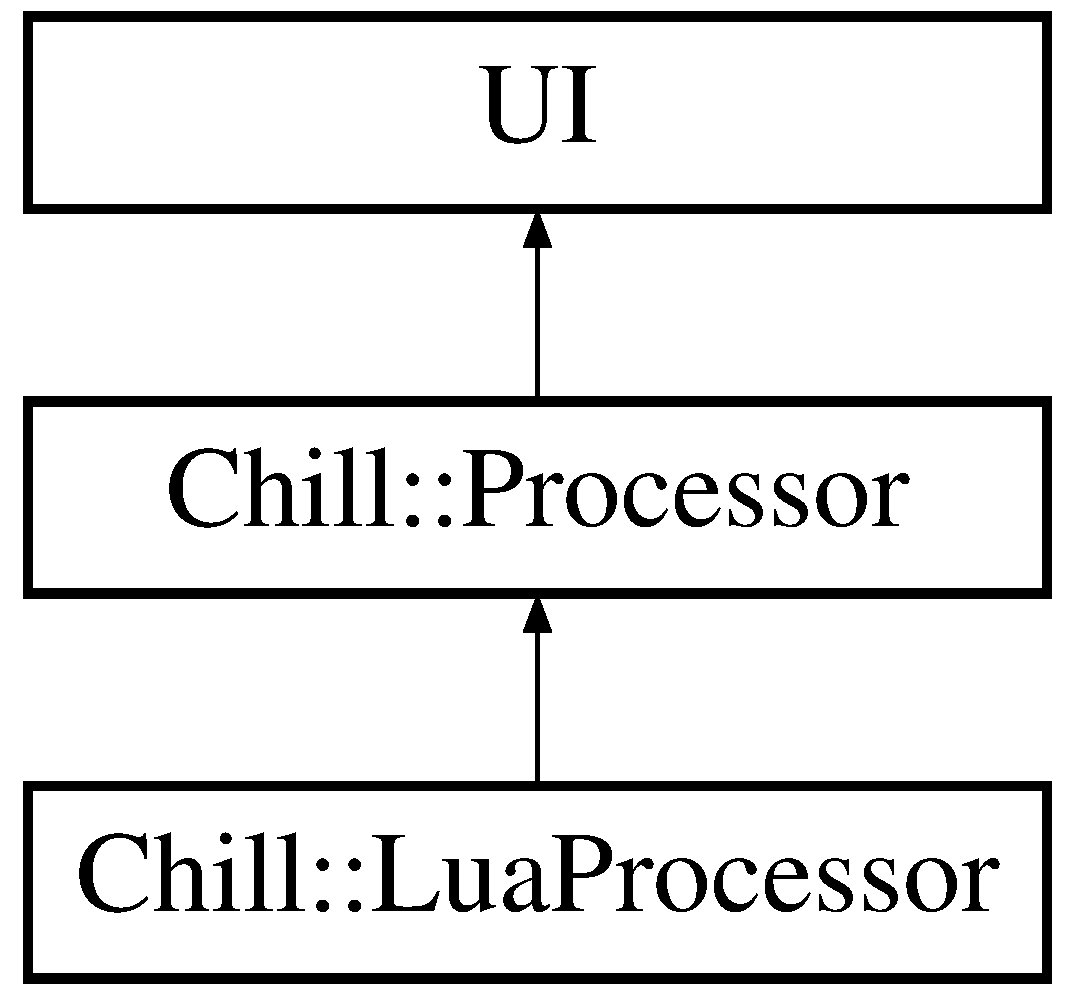
\includegraphics[height=3.000000cm]{class_chill_1_1_lua_processor}
\end{center}
\end{figure}
\subsection*{Public Member Functions}
\begin{DoxyCompactItemize}
\item 
\mbox{\Hypertarget{class_chill_1_1_lua_processor_a4f669bc7bb348a847b07bdcfb913a878}\label{class_chill_1_1_lua_processor_a4f669bc7bb348a847b07bdcfb913a878}} 
{\bfseries Lua\+Processor} (const std\+::string \&\+\_\+path)
\item 
\mbox{\Hypertarget{class_chill_1_1_lua_processor_a48195953233edfe7e77d2791789b8b4a}\label{class_chill_1_1_lua_processor_a48195953233edfe7e77d2791789b8b4a}} 
virtual Auto\+Ptr$<$ \mbox{\hyperlink{class_chill_1_1_processor}{Processor}} $>$ {\bfseries clone} () override
\end{DoxyCompactItemize}
\subsection*{Additional Inherited Members}


The documentation for this class was generated from the following files\+:\begin{DoxyCompactItemize}
\item 
E\+:/\+Chill/chill/chill\+Engine/\mbox{\hyperlink{_processor_8h}{Processor.\+h}}\item 
E\+:/\+Chill/chill/chill\+Engine/Lua\+Processor.\+cpp\end{DoxyCompactItemize}

\hypertarget{class_chill_1_1_multiplexer}{}\section{Chill\+:\+:Multiplexer Class Reference}
\label{class_chill_1_1_multiplexer}\index{Chill\+::\+Multiplexer@{Chill\+::\+Multiplexer}}
Inheritance diagram for Chill\+:\+:Multiplexer\+:\begin{figure}[H]
\begin{center}
\leavevmode
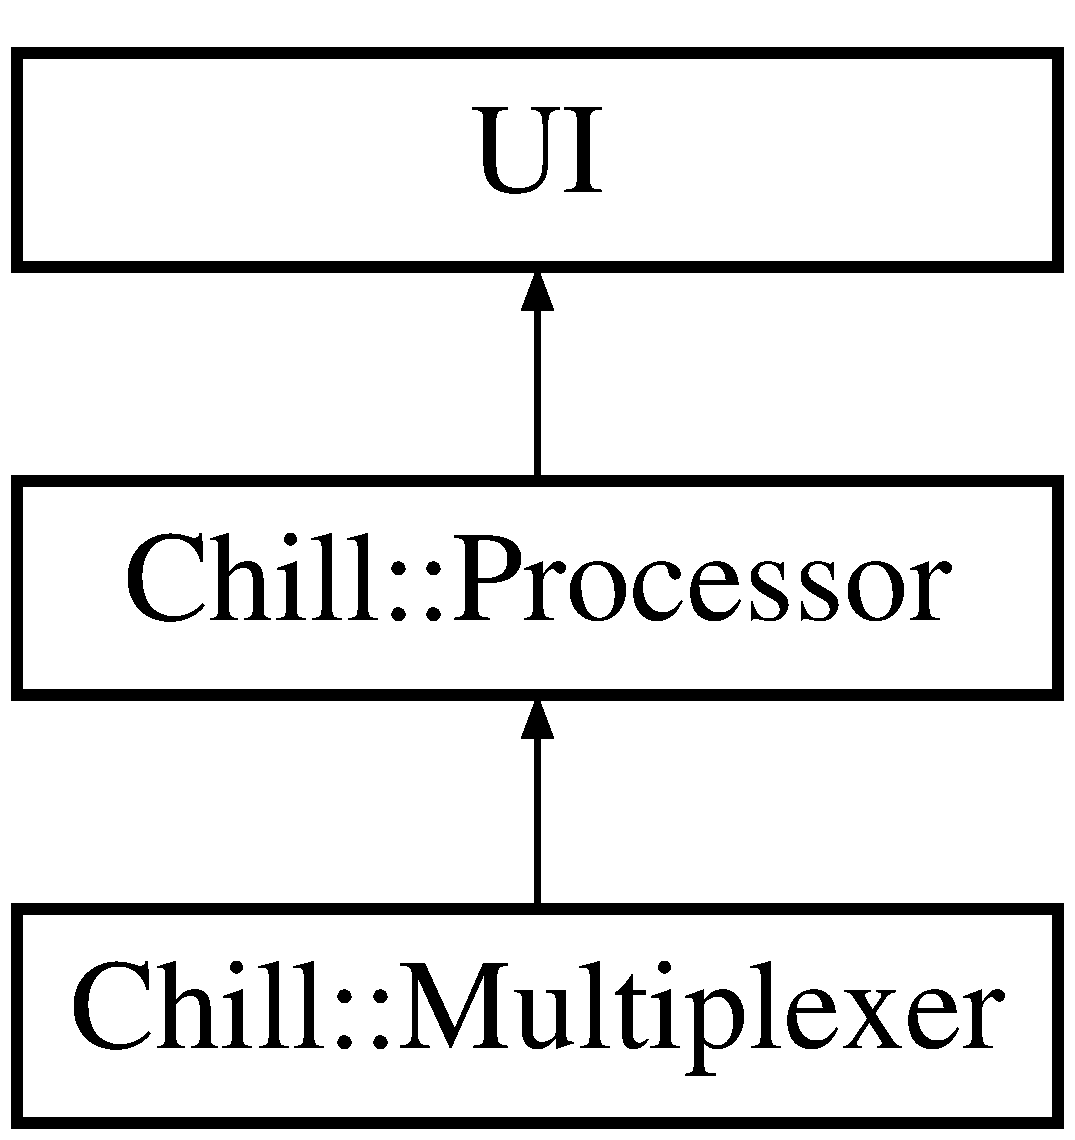
\includegraphics[height=3.000000cm]{class_chill_1_1_multiplexer}
\end{center}
\end{figure}
\subsection*{Public Member Functions}
\begin{DoxyCompactItemize}
\item 
\mbox{\Hypertarget{class_chill_1_1_multiplexer_a8320698e871a005ad9a5c1fbe00082e7}\label{class_chill_1_1_multiplexer_a8320698e871a005ad9a5c1fbe00082e7}} 
virtual Auto\+Ptr$<$ \mbox{\hyperlink{class_chill_1_1_processor}{Processor}} $>$ {\bfseries clone} () override
\item 
bool \mbox{\hyperlink{class_chill_1_1_multiplexer_aac8cf52a617091ffedaee970b5550270}{draw}} ()
\end{DoxyCompactItemize}
\subsection*{Additional Inherited Members}


\subsection{Member Function Documentation}
\mbox{\Hypertarget{class_chill_1_1_multiplexer_aac8cf52a617091ffedaee970b5550270}\label{class_chill_1_1_multiplexer_aac8cf52a617091ffedaee970b5550270}} 
\index{Chill\+::\+Multiplexer@{Chill\+::\+Multiplexer}!draw@{draw}}
\index{draw@{draw}!Chill\+::\+Multiplexer@{Chill\+::\+Multiplexer}}
\subsubsection{\texorpdfstring{draw()}{draw()}}
{\footnotesize\ttfamily bool Chill\+::\+Multiplexer\+::draw (\begin{DoxyParamCaption}{ }\end{DoxyParamCaption})\hspace{0.3cm}{\ttfamily [virtual]}}

Draw the processor 

Reimplemented from \mbox{\hyperlink{class_chill_1_1_processor_a2eb86d9750e1c0d5ac7f6da166aca8fd}{Chill\+::\+Processor}}.



The documentation for this class was generated from the following files\+:\begin{DoxyCompactItemize}
\item 
E\+:/\+Chill/chill/chill\+Engine/\mbox{\hyperlink{_processor_8h}{Processor.\+h}}\item 
E\+:/\+Chill/chill/chill\+Engine/Processor.\+cpp\end{DoxyCompactItemize}

\hypertarget{class_chill_1_1_node_editor}{}\section{Chill\+:\+:Node\+Editor Class Reference}
\label{class_chill_1_1_node_editor}\index{Chill\+::\+Node\+Editor@{Chill\+::\+Node\+Editor}}
Inheritance diagram for Chill\+:\+:Node\+Editor\+:\begin{figure}[H]
\begin{center}
\leavevmode
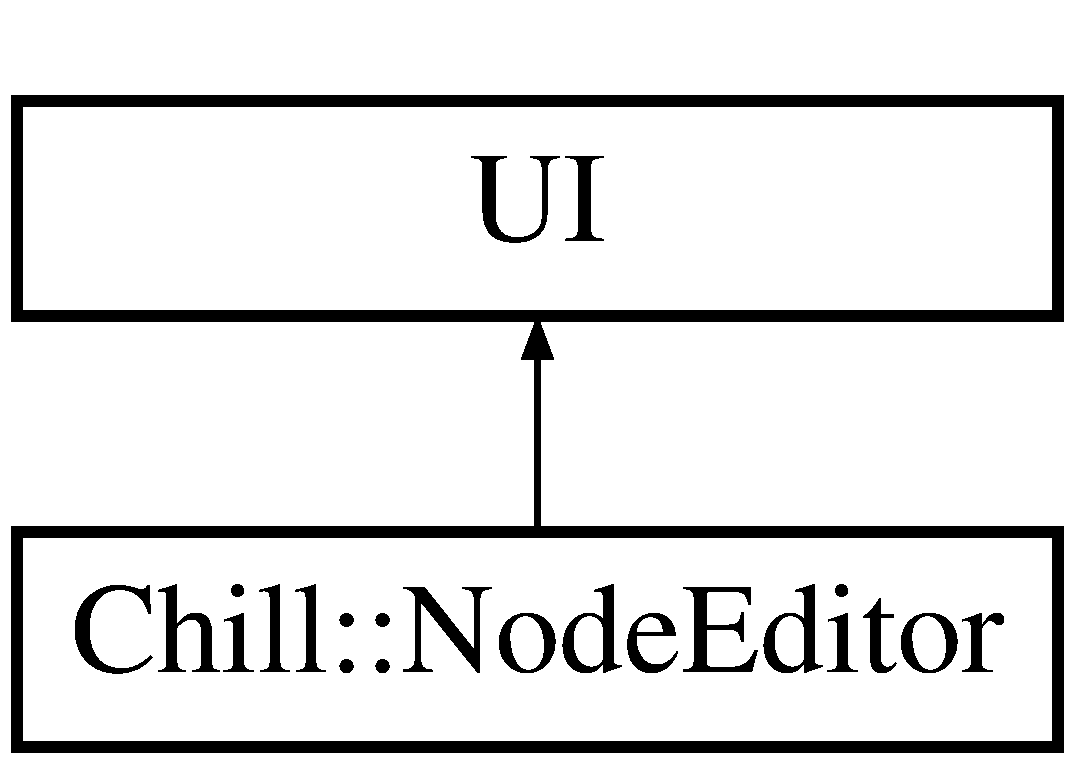
\includegraphics[height=2.000000cm]{class_chill_1_1_node_editor}
\end{center}
\end{figure}
\subsection*{Public Member Functions}
\begin{DoxyCompactItemize}
\item 
bool \mbox{\hyperlink{class_chill_1_1_node_editor_a7b67d5473c93d3258a2dc565e76da024}{draw}} ()
\item 
\mbox{\Hypertarget{class_chill_1_1_node_editor_a3670fbd563c836d91e0df519471e3c60}\label{class_chill_1_1_node_editor_a3670fbd563c836d91e0df519471e3c60}} 
void {\bfseries draw\+Menu\+Bar} ()
\item 
\mbox{\Hypertarget{class_chill_1_1_node_editor_a2119a9f6e2041ba91deb36a1b45a8e13}\label{class_chill_1_1_node_editor_a2119a9f6e2041ba91deb36a1b45a8e13}} 
void {\bfseries draw\+Left\+Menu} ()
\item 
\mbox{\Hypertarget{class_chill_1_1_node_editor_ae5938466153e88151b86f71e42019007}\label{class_chill_1_1_node_editor_ae5938466153e88151b86f71e42019007}} 
void {\bfseries draw\+Graph} ()
\item 
\mbox{\Hypertarget{class_chill_1_1_node_editor_ae16b6f9169e6be3c66b0bbb16d98478e}\label{class_chill_1_1_node_editor_ae16b6f9169e6be3c66b0bbb16d98478e}} 
\mbox{\hyperlink{class_chill_1_1_processing_graph}{Processing\+Graph}} $\ast$ {\bfseries get\+Current\+Graph} ()
\item 
\mbox{\Hypertarget{class_chill_1_1_node_editor_ac4ce7407055b993d07acc52be4c0d7d4}\label{class_chill_1_1_node_editor_ac4ce7407055b993d07acc52be4c0d7d4}} 
\mbox{\hyperlink{class_chill_1_1_processing_graph}{Processing\+Graph}} $\ast$ {\bfseries get\+Main\+Graph} ()
\item 
\mbox{\Hypertarget{class_chill_1_1_node_editor_afb0b4e46c302e32949fe910a395f768d}\label{class_chill_1_1_node_editor_afb0b4e46c302e32949fe910a395f768d}} 
void {\bfseries set\+Main\+Graph} (\mbox{\hyperlink{class_chill_1_1_processing_graph}{Processing\+Graph}} $\ast$\+\_\+graph)
\item 
\mbox{\Hypertarget{class_chill_1_1_node_editor_ad97dd216359065bab711ccb8f9085998}\label{class_chill_1_1_node_editor_ad97dd216359065bab711ccb8f9085998}} 
void {\bfseries set\+Selected\+Input} (Auto\+Ptr$<$ \mbox{\hyperlink{class_chill_1_1_processor_input}{Processor\+Input}} $>$ \+\_\+input)
\item 
\mbox{\Hypertarget{class_chill_1_1_node_editor_aa6e12a25a6abc55d4a5b2350f73f5c21}\label{class_chill_1_1_node_editor_aa6e12a25a6abc55d4a5b2350f73f5c21}} 
Auto\+Ptr$<$ \mbox{\hyperlink{class_chill_1_1_processor_input}{Processor\+Input}} $>$ {\bfseries get\+Selected\+Input} ()
\item 
\mbox{\Hypertarget{class_chill_1_1_node_editor_a3d3c6eb135f7a258b62d60eda8894d03}\label{class_chill_1_1_node_editor_a3d3c6eb135f7a258b62d60eda8894d03}} 
void {\bfseries set\+Selected\+Output} (Auto\+Ptr$<$ \mbox{\hyperlink{class_chill_1_1_processor_output}{Processor\+Output}} $>$ \+\_\+output)
\item 
\mbox{\Hypertarget{class_chill_1_1_node_editor_a8a906341d76dc5fa8a8ea85b45fd4680}\label{class_chill_1_1_node_editor_a8a906341d76dc5fa8a8ea85b45fd4680}} 
Auto\+Ptr$<$ \mbox{\hyperlink{class_chill_1_1_processor_output}{Processor\+Output}} $>$ {\bfseries get\+Selected\+Output} ()
\end{DoxyCompactItemize}
\subsection*{Static Public Member Functions}
\begin{DoxyCompactItemize}
\item 
\mbox{\Hypertarget{class_chill_1_1_node_editor_a36965a05441d70eabf6ca4313ec127a6}\label{class_chill_1_1_node_editor_a36965a05441d70eabf6ca4313ec127a6}} 
static void {\bfseries Node\+Editor\+::launch} ()
\item 
\mbox{\Hypertarget{class_chill_1_1_node_editor_ab1f2859cc0841b13290a1f1cb3516965}\label{class_chill_1_1_node_editor_ab1f2859cc0841b13290a1f1cb3516965}} 
static \mbox{\hyperlink{class_chill_1_1_node_editor}{Node\+Editor}} $\ast$ {\bfseries Instance} ()
\item 
static void \mbox{\hyperlink{class_chill_1_1_node_editor_accabf149df9cb481956ef3c0132252f8}{main\+Render}} ()
\item 
static void \mbox{\hyperlink{class_chill_1_1_node_editor_a94f29235392656e4c60c3aa0d81c646a}{main\+On\+Resize}} (uint \+\_\+width, uint \+\_\+height)
\item 
static void \mbox{\hyperlink{class_chill_1_1_node_editor_a0abdd4a4d4026177be77a8e59f4aa5cf}{main\+Key\+Pressed}} (uchar \+\_\+k)
\item 
\mbox{\Hypertarget{class_chill_1_1_node_editor_a5033568fec5142f98f6cd6881a38103f}\label{class_chill_1_1_node_editor_a5033568fec5142f98f6cd6881a38103f}} 
static void {\bfseries main\+Scan\+Code\+Pressed} (uint \+\_\+sc)
\item 
\mbox{\Hypertarget{class_chill_1_1_node_editor_ac47a6c0b50d9105e34c39aaf66c8c28f}\label{class_chill_1_1_node_editor_ac47a6c0b50d9105e34c39aaf66c8c28f}} 
static void {\bfseries main\+Scan\+Code\+Unpressed} (uint \+\_\+sc)
\item 
\mbox{\Hypertarget{class_chill_1_1_node_editor_a61540bc669952d0fe214de5e82e50ec3}\label{class_chill_1_1_node_editor_a61540bc669952d0fe214de5e82e50ec3}} 
static void {\bfseries main\+Mouse\+Moved} (uint \+\_\+x, uint \+\_\+y)
\item 
\mbox{\Hypertarget{class_chill_1_1_node_editor_af01b8b889b0e9182c9ab3e3fa58f0320}\label{class_chill_1_1_node_editor_af01b8b889b0e9182c9ab3e3fa58f0320}} 
static void {\bfseries main\+Mouse\+Pressed} (uint \+\_\+x, uint \+\_\+y, uint \+\_\+button, uint \+\_\+flags)
\end{DoxyCompactItemize}
\subsection*{Additional Inherited Members}


\subsection{Member Function Documentation}
\mbox{\Hypertarget{class_chill_1_1_node_editor_a7b67d5473c93d3258a2dc565e76da024}\label{class_chill_1_1_node_editor_a7b67d5473c93d3258a2dc565e76da024}} 
\index{Chill\+::\+Node\+Editor@{Chill\+::\+Node\+Editor}!draw@{draw}}
\index{draw@{draw}!Chill\+::\+Node\+Editor@{Chill\+::\+Node\+Editor}}
\subsubsection{\texorpdfstring{draw()}{draw()}}
{\footnotesize\ttfamily bool Chill\+::\+Node\+Editor\+::draw (\begin{DoxyParamCaption}{ }\end{DoxyParamCaption})\hspace{0.3cm}{\ttfamily [virtual]}}

Draw the component return true if the element is rendered, else false 

Implements \mbox{\hyperlink{class_u_i_a5025b88e26f21852c0cd2e4b42675c50}{UI}}.

\mbox{\Hypertarget{class_chill_1_1_node_editor_a0abdd4a4d4026177be77a8e59f4aa5cf}\label{class_chill_1_1_node_editor_a0abdd4a4d4026177be77a8e59f4aa5cf}} 
\index{Chill\+::\+Node\+Editor@{Chill\+::\+Node\+Editor}!main\+Key\+Pressed@{main\+Key\+Pressed}}
\index{main\+Key\+Pressed@{main\+Key\+Pressed}!Chill\+::\+Node\+Editor@{Chill\+::\+Node\+Editor}}
\subsubsection{\texorpdfstring{main\+Key\+Pressed()}{mainKeyPressed()}}
{\footnotesize\ttfamily void Chill\+::\+Node\+Editor\+::main\+Key\+Pressed (\begin{DoxyParamCaption}\item[{uchar}]{\+\_\+k }\end{DoxyParamCaption})\hspace{0.3cm}{\ttfamily [static]}}

Called when a key is pressed 
\begin{DoxyParams}{Parameters}
{\em k} & the typed character \\
\hline
\end{DoxyParams}
\mbox{\Hypertarget{class_chill_1_1_node_editor_a94f29235392656e4c60c3aa0d81c646a}\label{class_chill_1_1_node_editor_a94f29235392656e4c60c3aa0d81c646a}} 
\index{Chill\+::\+Node\+Editor@{Chill\+::\+Node\+Editor}!main\+On\+Resize@{main\+On\+Resize}}
\index{main\+On\+Resize@{main\+On\+Resize}!Chill\+::\+Node\+Editor@{Chill\+::\+Node\+Editor}}
\subsubsection{\texorpdfstring{main\+On\+Resize()}{mainOnResize()}}
{\footnotesize\ttfamily void Chill\+::\+Node\+Editor\+::main\+On\+Resize (\begin{DoxyParamCaption}\item[{uint}]{\+\_\+width,  }\item[{uint}]{\+\_\+height }\end{DoxyParamCaption})\hspace{0.3cm}{\ttfamily [static]}}

Called on resize 
\begin{DoxyParams}{Parameters}
{\em width} & the new width \\
\hline
{\em height} & the new height \\
\hline
\end{DoxyParams}
\mbox{\Hypertarget{class_chill_1_1_node_editor_accabf149df9cb481956ef3c0132252f8}\label{class_chill_1_1_node_editor_accabf149df9cb481956ef3c0132252f8}} 
\index{Chill\+::\+Node\+Editor@{Chill\+::\+Node\+Editor}!main\+Render@{main\+Render}}
\index{main\+Render@{main\+Render}!Chill\+::\+Node\+Editor@{Chill\+::\+Node\+Editor}}
\subsubsection{\texorpdfstring{main\+Render()}{mainRender()}}
{\footnotesize\ttfamily void Chill\+::\+Node\+Editor\+::main\+Render (\begin{DoxyParamCaption}{ }\end{DoxyParamCaption})\hspace{0.3cm}{\ttfamily [static]}}

Called at each frame 

The documentation for this class was generated from the following files\+:\begin{DoxyCompactItemize}
\item 
E\+:/\+Chill/chill/chill\+Engine/Node\+Editor.\+h\item 
E\+:/\+Chill/chill/chill\+Engine/Node\+Editor.\+cpp\end{DoxyCompactItemize}

\hypertarget{class_chill_1_1_processing_graph}{}\section{Chill\+:\+:Processing\+Graph Class Reference}
\label{class_chill_1_1_processing_graph}\index{Chill\+::\+Processing\+Graph@{Chill\+::\+Processing\+Graph}}


{\ttfamily \#include $<$Processing\+Graph.\+h$>$}

Inheritance diagram for Chill\+:\+:Processing\+Graph\+:\begin{figure}[H]
\begin{center}
\leavevmode
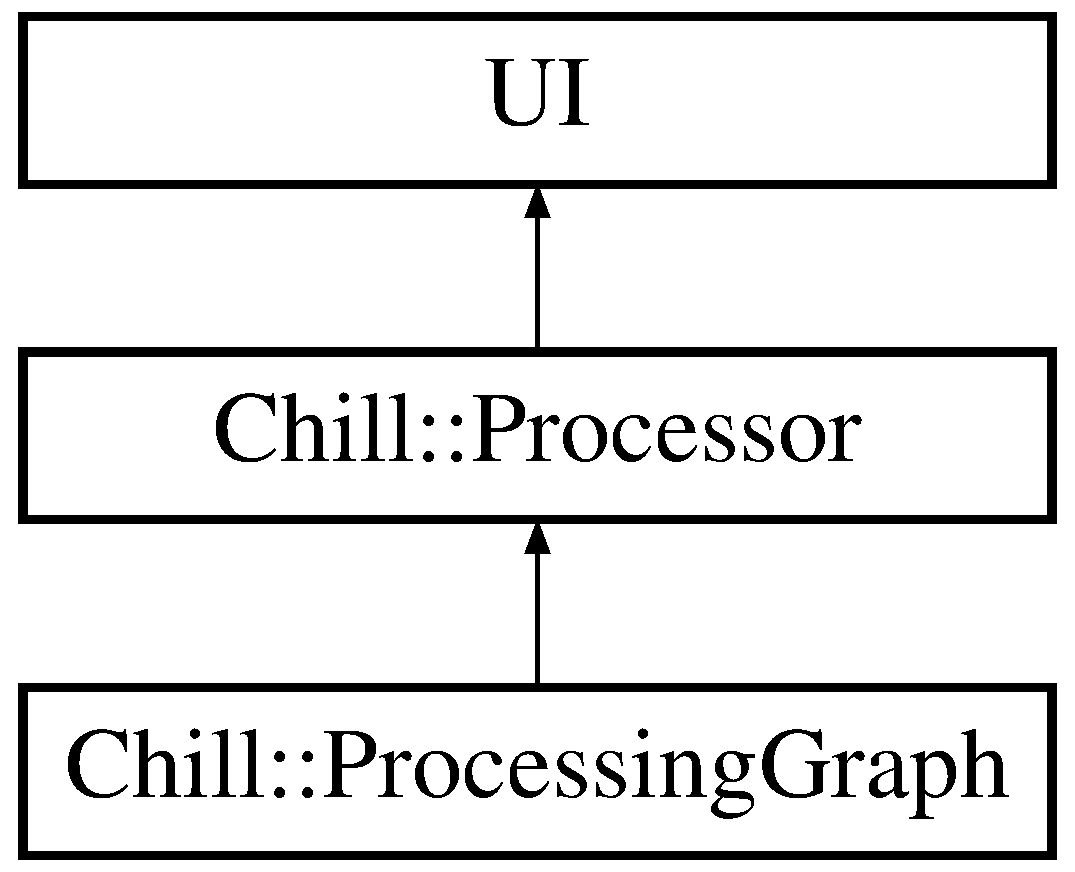
\includegraphics[height=3.000000cm]{class_chill_1_1_processing_graph}
\end{center}
\end{figure}
\subsection*{Public Member Functions}
\begin{DoxyCompactItemize}
\item 
\mbox{\Hypertarget{class_chill_1_1_processing_graph_a9fe5417596816aa6fea1c39abe9926c0}\label{class_chill_1_1_processing_graph_a9fe5417596816aa6fea1c39abe9926c0}} 
{\bfseries Processing\+Graph} (const std\+::string \&\+\_\+name)
\item 
{\footnotesize template$<$typename T\+\_\+\+Processor $>$ }\\Auto\+Ptr$<$ T\+\_\+\+Processor $>$ \mbox{\hyperlink{class_chill_1_1_processing_graph_aa3bd2de51d11a08d4de2f0230f7b65d4}{add\+Processor}} ()
\item 
void \mbox{\hyperlink{class_chill_1_1_processing_graph_a066ca6f9163fe4742254b9e6e7ccc857}{add\+Processor}} (Auto\+Ptr$<$ \mbox{\hyperlink{class_chill_1_1_processor}{Processor}} $>$ \+\_\+processor)
\item 
void \mbox{\hyperlink{class_chill_1_1_processing_graph_a7fe61b40e3ef530f9684600f3a93f53f}{remove\+Processor}} (Auto\+Ptr$<$ \mbox{\hyperlink{class_chill_1_1_processor}{Processor}} $>$ \&\+\_\+processor)
\item 
Auto\+Ptr$<$ \mbox{\hyperlink{class_chill_1_1_processing_graph}{Processing\+Graph}} $>$ \mbox{\hyperlink{class_chill_1_1_processing_graph_aa57e688eefcad73aa5880afa97a4c179}{copy\+Subset}} (const std\+::vector$<$ Auto\+Ptr$<$ \mbox{\hyperlink{class_chill_1_1_processor}{Processor}} $>$$>$ \&\+\_\+subset)
\item 
Auto\+Ptr$<$ \mbox{\hyperlink{class_chill_1_1_processing_graph}{Processing\+Graph}} $>$ \mbox{\hyperlink{class_chill_1_1_processing_graph_ad7554bc478052d49fc37d8d15e29827b}{collapse\+Subset}} (const std\+::vector$<$ Auto\+Ptr$<$ \mbox{\hyperlink{class_chill_1_1_processor}{Processor}} $>$$>$ \&\+\_\+subset)
\item 
void \mbox{\hyperlink{class_chill_1_1_processing_graph_a7a7185106dc9e412a870915ee956bcca}{expand\+Graph}} (Auto\+Ptr$<$ \mbox{\hyperlink{class_chill_1_1_processing_graph}{Processing\+Graph}} $>$ \&\+\_\+graph, Im\+Vec2 \+\_\+position)
\item 
\mbox{\Hypertarget{class_chill_1_1_processing_graph_a983f5286b3fff6252fb2d8226a6d5816}\label{class_chill_1_1_processing_graph_a983f5286b3fff6252fb2d8226a6d5816}} 
void {\bfseries add\+Proxy} (Auto\+Ptr$<$ \mbox{\hyperlink{class_chill_1_1_processor_output}{Processor\+Output}} $>$ \+\_\+proxy\+\_\+o, Auto\+Ptr$<$ \mbox{\hyperlink{class_chill_1_1_processor_input}{Processor\+Input}} $>$ \+\_\+proxy\+\_\+i)
\item 
\mbox{\Hypertarget{class_chill_1_1_processing_graph_ab870a61bcd6d90c2dde3bd06305b8f81}\label{class_chill_1_1_processing_graph_ab870a61bcd6d90c2dde3bd06305b8f81}} 
void {\bfseries add\+Proxy} (Auto\+Ptr$<$ \mbox{\hyperlink{class_chill_1_1_processor_input}{Processor\+Input}} $>$ \+\_\+proxy\+\_\+i, Auto\+Ptr$<$ \mbox{\hyperlink{class_chill_1_1_processor_output}{Processor\+Output}} $>$ \+\_\+proxy\+\_\+o)
\item 
const std\+::vector$<$ Auto\+Ptr$<$ \mbox{\hyperlink{class_chill_1_1_processor}{Processor}} $>$ $>$ \mbox{\hyperlink{class_chill_1_1_processing_graph_a5a999e6f0f2af8d67e2c3d0afb393707}{processors}} ()
\item 
\mbox{\Hypertarget{class_chill_1_1_processing_graph_aa3b30207dcfbe5271a55ac7349bb9a36}\label{class_chill_1_1_processing_graph_aa3b30207dcfbe5271a55ac7349bb9a36}} 
Auto\+Ptr$<$ \mbox{\hyperlink{class_chill_1_1_processor}{Processor}} $>$ {\bfseries clone} ()
\item 
void \mbox{\hyperlink{class_chill_1_1_processing_graph_a15ebc74e61a5bbdba8715c8d93b2815d}{save}} (std\+::ofstream \&\+\_\+stream)
\item 
\mbox{\Hypertarget{class_chill_1_1_processing_graph_a35a0eb123e8bfc04838377a4c02d9d71}\label{class_chill_1_1_processing_graph_a35a0eb123e8bfc04838377a4c02d9d71}} 
Im\+Vec2 {\bfseries get\+Barycenter} (std\+::vector$<$ Auto\+Ptr$<$ \mbox{\hyperlink{class_chill_1_1_processor}{Processor}} $>$$>$ \+\_\+processors)
\item 
\mbox{\Hypertarget{class_chill_1_1_processing_graph_a8e2059c2764aa879d831ff9d437cd532}\label{class_chill_1_1_processing_graph_a8e2059c2764aa879d831ff9d437cd532}} 
Im\+Vec2 {\bfseries get\+Barycenter} ()
\item 
\mbox{\Hypertarget{class_chill_1_1_processing_graph_a07394d72254516ed9250516f921ce02b}\label{class_chill_1_1_processing_graph_a07394d72254516ed9250516f921ce02b}} 
A\+A\+Box {\bfseries get\+Bounding\+Box} (std\+::vector$<$ Auto\+Ptr$<$ \mbox{\hyperlink{class_chill_1_1_processor}{Processor}} $>$$>$ \+\_\+processors)
\end{DoxyCompactItemize}
\subsection*{Static Public Member Functions}
\begin{DoxyCompactItemize}
\item 
static bool \mbox{\hyperlink{class_chill_1_1_processing_graph_a5af6528fa4dd66f6c59dc6144a70d4c3}{connect}} (const Auto\+Ptr$<$ \mbox{\hyperlink{class_chill_1_1_processor}{Processor}} $>$ \&\+\_\+from, const std\+::string \+\_\+output\+\_\+name, const Auto\+Ptr$<$ \mbox{\hyperlink{class_chill_1_1_processor}{Processor}} $>$ \&\+\_\+to, const std\+::string \+\_\+input\+\_\+name)
\item 
static bool \mbox{\hyperlink{class_chill_1_1_processing_graph_a7f61e70c0b6e36b463108c78ab6ff82c}{connect}} (Auto\+Ptr$<$ \mbox{\hyperlink{class_chill_1_1_processor_output}{Processor\+Output}} $>$ \&\+\_\+from, Auto\+Ptr$<$ \mbox{\hyperlink{class_chill_1_1_processor_input}{Processor\+Input}} $>$ \&\+\_\+to)
\item 
static void \mbox{\hyperlink{class_chill_1_1_processing_graph_a9f3ccb8d44f098a9728059f839e86580}{disconnect}} (Auto\+Ptr$<$ \mbox{\hyperlink{class_chill_1_1_processor_input}{Processor\+Input}} $>$ \&\+\_\+to)
\item 
static void \mbox{\hyperlink{class_chill_1_1_processing_graph_a907f3d1f85ba8a59ecd5ab0aa8b353ee}{disconnect}} (Auto\+Ptr$<$ \mbox{\hyperlink{class_chill_1_1_processor_output}{Processor\+Output}} $>$ \&\+\_\+from)
\item 
\mbox{\Hypertarget{class_chill_1_1_processing_graph_a9919fe8ff6b7229a77eb9060b0af2ebb}\label{class_chill_1_1_processing_graph_a9919fe8ff6b7229a77eb9060b0af2ebb}} 
static bool {\bfseries are\+Connected} (\mbox{\hyperlink{class_chill_1_1_processor}{Processor}} $\ast$\+\_\+from, \mbox{\hyperlink{class_chill_1_1_processor}{Processor}} $\ast$\+\_\+to)
\end{DoxyCompactItemize}
\subsection*{Protected Attributes}
\begin{DoxyCompactItemize}
\item 
std\+::vector$<$ Auto\+Ptr$<$ \mbox{\hyperlink{class_chill_1_1_processor}{Processor}} $>$ $>$ \mbox{\hyperlink{class_chill_1_1_processing_graph_a14b37b603b274ee9e74ccc2fecd61850}{m\+\_\+processors}}
\item 
std\+::vector$<$ Group\+Input $>$ \mbox{\hyperlink{class_chill_1_1_processing_graph_a45eaab4f6bbecd08837b4ef01f320719}{m\+\_\+group\+\_\+inputs}}
\item 
std\+::vector$<$ Group\+Output $>$ \mbox{\hyperlink{class_chill_1_1_processing_graph_af45053cb80e67bab58725bf2137e2d30}{m\+\_\+group\+\_\+outputs}}
\end{DoxyCompactItemize}
\subsection*{Additional Inherited Members}


\subsection{Detailed Description}
Graph class. Contains all nodes and connections. 

\subsection{Member Function Documentation}
\mbox{\Hypertarget{class_chill_1_1_processing_graph_aa3bd2de51d11a08d4de2f0230f7b65d4}\label{class_chill_1_1_processing_graph_aa3bd2de51d11a08d4de2f0230f7b65d4}} 
\index{Chill\+::\+Processing\+Graph@{Chill\+::\+Processing\+Graph}!add\+Processor@{add\+Processor}}
\index{add\+Processor@{add\+Processor}!Chill\+::\+Processing\+Graph@{Chill\+::\+Processing\+Graph}}
\subsubsection{\texorpdfstring{add\+Processor()}{addProcessor()}\hspace{0.1cm}{\footnotesize\ttfamily [1/2]}}
{\footnotesize\ttfamily template$<$typename T\+\_\+\+Processor $>$ \\
Auto\+Ptr$<$T\+\_\+\+Processor$>$ Chill\+::\+Processing\+Graph\+::add\+Processor (\begin{DoxyParamCaption}{ }\end{DoxyParamCaption})\hspace{0.3cm}{\ttfamily [inline]}}

Add a new processor to the graph. \begin{DoxyReturn}{Returns}
The Auto\+Ptr related to the processor created. 
\end{DoxyReturn}
\mbox{\Hypertarget{class_chill_1_1_processing_graph_a066ca6f9163fe4742254b9e6e7ccc857}\label{class_chill_1_1_processing_graph_a066ca6f9163fe4742254b9e6e7ccc857}} 
\index{Chill\+::\+Processing\+Graph@{Chill\+::\+Processing\+Graph}!add\+Processor@{add\+Processor}}
\index{add\+Processor@{add\+Processor}!Chill\+::\+Processing\+Graph@{Chill\+::\+Processing\+Graph}}
\subsubsection{\texorpdfstring{add\+Processor()}{addProcessor()}\hspace{0.1cm}{\footnotesize\ttfamily [2/2]}}
{\footnotesize\ttfamily void Chill\+::\+Processing\+Graph\+::add\+Processor (\begin{DoxyParamCaption}\item[{Auto\+Ptr$<$ \mbox{\hyperlink{class_chill_1_1_processor}{Processor}} $>$}]{\+\_\+processor }\end{DoxyParamCaption})\hspace{0.3cm}{\ttfamily [inline]}}

Add an existing processor to the graph. 
\begin{DoxyParams}{Parameters}
{\em \+\_\+processor} & The Auto\+Ptr related to the processor. \\
\hline
\end{DoxyParams}
\mbox{\Hypertarget{class_chill_1_1_processing_graph_ad7554bc478052d49fc37d8d15e29827b}\label{class_chill_1_1_processing_graph_ad7554bc478052d49fc37d8d15e29827b}} 
\index{Chill\+::\+Processing\+Graph@{Chill\+::\+Processing\+Graph}!collapse\+Subset@{collapse\+Subset}}
\index{collapse\+Subset@{collapse\+Subset}!Chill\+::\+Processing\+Graph@{Chill\+::\+Processing\+Graph}}
\subsubsection{\texorpdfstring{collapse\+Subset()}{collapseSubset()}}
{\footnotesize\ttfamily Auto\+Ptr$<$ \mbox{\hyperlink{class_chill_1_1_processing_graph}{Processing\+Graph}} $>$ Chill\+::\+Processing\+Graph\+::collapse\+Subset (\begin{DoxyParamCaption}\item[{const std\+::vector$<$ Auto\+Ptr$<$ \mbox{\hyperlink{class_chill_1_1_processor}{Processor}} $>$$>$ \&}]{\+\_\+subset }\end{DoxyParamCaption})}

Move all the processors inside a new graph. All connections that are outside of this graph are connected to the new processor. 
\begin{DoxyParams}{Parameters}
{\em \+\_\+subset} & The list of processors to collapse. \\
\hline
\end{DoxyParams}
\begin{DoxyReturn}{Returns}
A new graph which contains all those processors. 
\end{DoxyReturn}
\mbox{\Hypertarget{class_chill_1_1_processing_graph_a5af6528fa4dd66f6c59dc6144a70d4c3}\label{class_chill_1_1_processing_graph_a5af6528fa4dd66f6c59dc6144a70d4c3}} 
\index{Chill\+::\+Processing\+Graph@{Chill\+::\+Processing\+Graph}!connect@{connect}}
\index{connect@{connect}!Chill\+::\+Processing\+Graph@{Chill\+::\+Processing\+Graph}}
\subsubsection{\texorpdfstring{connect()}{connect()}\hspace{0.1cm}{\footnotesize\ttfamily [1/2]}}
{\footnotesize\ttfamily bool Chill\+::\+Processing\+Graph\+::connect (\begin{DoxyParamCaption}\item[{const Auto\+Ptr$<$ \mbox{\hyperlink{class_chill_1_1_processor}{Processor}} $>$ \&}]{\+\_\+from,  }\item[{const std\+::string}]{\+\_\+output\+\_\+name,  }\item[{const Auto\+Ptr$<$ \mbox{\hyperlink{class_chill_1_1_processor}{Processor}} $>$ \&}]{\+\_\+to,  }\item[{const std\+::string}]{\+\_\+input\+\_\+name }\end{DoxyParamCaption})\hspace{0.3cm}{\ttfamily [static]}}

Add a new connection to the graph if, and only if, there is no cycle created. 
\begin{DoxyParams}{Parameters}
{\em \+\_\+from} & The origin processor. \\
\hline
{\em \+\_\+output\+\_\+name} & The name of the output. \\
\hline
{\em \+\_\+to} & The destination processor. \\
\hline
{\em \+\_\+input\+\_\+name} & The name of the input. \\
\hline
\end{DoxyParams}
\mbox{\Hypertarget{class_chill_1_1_processing_graph_a7f61e70c0b6e36b463108c78ab6ff82c}\label{class_chill_1_1_processing_graph_a7f61e70c0b6e36b463108c78ab6ff82c}} 
\index{Chill\+::\+Processing\+Graph@{Chill\+::\+Processing\+Graph}!connect@{connect}}
\index{connect@{connect}!Chill\+::\+Processing\+Graph@{Chill\+::\+Processing\+Graph}}
\subsubsection{\texorpdfstring{connect()}{connect()}\hspace{0.1cm}{\footnotesize\ttfamily [2/2]}}
{\footnotesize\ttfamily bool Chill\+::\+Processing\+Graph\+::connect (\begin{DoxyParamCaption}\item[{Auto\+Ptr$<$ \mbox{\hyperlink{class_chill_1_1_processor_output}{Processor\+Output}} $>$ \&}]{\+\_\+from,  }\item[{Auto\+Ptr$<$ \mbox{\hyperlink{class_chill_1_1_processor_input}{Processor\+Input}} $>$ \&}]{\+\_\+to }\end{DoxyParamCaption})\hspace{0.3cm}{\ttfamily [static]}}

Add a new connection to the graph if, and only if, there is no cycle created. 
\begin{DoxyParams}{Parameters}
{\em \+\_\+from} & The processor\textquotesingle{}s output. \\
\hline
{\em \+\_\+to} & The processor\textquotesingle{}s input. \\
\hline
\end{DoxyParams}
\mbox{\Hypertarget{class_chill_1_1_processing_graph_aa57e688eefcad73aa5880afa97a4c179}\label{class_chill_1_1_processing_graph_aa57e688eefcad73aa5880afa97a4c179}} 
\index{Chill\+::\+Processing\+Graph@{Chill\+::\+Processing\+Graph}!copy\+Subset@{copy\+Subset}}
\index{copy\+Subset@{copy\+Subset}!Chill\+::\+Processing\+Graph@{Chill\+::\+Processing\+Graph}}
\subsubsection{\texorpdfstring{copy\+Subset()}{copySubset()}}
{\footnotesize\ttfamily Auto\+Ptr$<$ \mbox{\hyperlink{class_chill_1_1_processing_graph}{Processing\+Graph}} $>$ Chill\+::\+Processing\+Graph\+::copy\+Subset (\begin{DoxyParamCaption}\item[{const std\+::vector$<$ Auto\+Ptr$<$ \mbox{\hyperlink{class_chill_1_1_processor}{Processor}} $>$$>$ \&}]{\+\_\+subset }\end{DoxyParamCaption})}

Duplicate a set of nodes. All connections that are outside of this set are not duplicated. 
\begin{DoxyParams}{Parameters}
{\em \+\_\+subset} & The list of processors to duplicate. \\
\hline
\end{DoxyParams}
\begin{DoxyReturn}{Returns}
A new graph which contains all those processors. 
\end{DoxyReturn}
\mbox{\Hypertarget{class_chill_1_1_processing_graph_a9f3ccb8d44f098a9728059f839e86580}\label{class_chill_1_1_processing_graph_a9f3ccb8d44f098a9728059f839e86580}} 
\index{Chill\+::\+Processing\+Graph@{Chill\+::\+Processing\+Graph}!disconnect@{disconnect}}
\index{disconnect@{disconnect}!Chill\+::\+Processing\+Graph@{Chill\+::\+Processing\+Graph}}
\subsubsection{\texorpdfstring{disconnect()}{disconnect()}\hspace{0.1cm}{\footnotesize\ttfamily [1/2]}}
{\footnotesize\ttfamily void Chill\+::\+Processing\+Graph\+::disconnect (\begin{DoxyParamCaption}\item[{Auto\+Ptr$<$ \mbox{\hyperlink{class_chill_1_1_processor_input}{Processor\+Input}} $>$ \&}]{\+\_\+to }\end{DoxyParamCaption})\hspace{0.3cm}{\ttfamily [static]}}

Remove a connection in the graph. 
\begin{DoxyParams}{Parameters}
{\em \+\_\+to} & The processor\textquotesingle{}s input. \\
\hline
\end{DoxyParams}
\mbox{\Hypertarget{class_chill_1_1_processing_graph_a907f3d1f85ba8a59ecd5ab0aa8b353ee}\label{class_chill_1_1_processing_graph_a907f3d1f85ba8a59ecd5ab0aa8b353ee}} 
\index{Chill\+::\+Processing\+Graph@{Chill\+::\+Processing\+Graph}!disconnect@{disconnect}}
\index{disconnect@{disconnect}!Chill\+::\+Processing\+Graph@{Chill\+::\+Processing\+Graph}}
\subsubsection{\texorpdfstring{disconnect()}{disconnect()}\hspace{0.1cm}{\footnotesize\ttfamily [2/2]}}
{\footnotesize\ttfamily void Chill\+::\+Processing\+Graph\+::disconnect (\begin{DoxyParamCaption}\item[{Auto\+Ptr$<$ \mbox{\hyperlink{class_chill_1_1_processor_output}{Processor\+Output}} $>$ \&}]{\+\_\+from }\end{DoxyParamCaption})\hspace{0.3cm}{\ttfamily [static]}}

Remove a connection in the graph. 
\begin{DoxyParams}{Parameters}
{\em \+\_\+from} & The processor\textquotesingle{}s output. \\
\hline
\end{DoxyParams}
\mbox{\Hypertarget{class_chill_1_1_processing_graph_a7a7185106dc9e412a870915ee956bcca}\label{class_chill_1_1_processing_graph_a7a7185106dc9e412a870915ee956bcca}} 
\index{Chill\+::\+Processing\+Graph@{Chill\+::\+Processing\+Graph}!expand\+Graph@{expand\+Graph}}
\index{expand\+Graph@{expand\+Graph}!Chill\+::\+Processing\+Graph@{Chill\+::\+Processing\+Graph}}
\subsubsection{\texorpdfstring{expand\+Graph()}{expandGraph()}}
{\footnotesize\ttfamily void Chill\+::\+Processing\+Graph\+::expand\+Graph (\begin{DoxyParamCaption}\item[{Auto\+Ptr$<$ \mbox{\hyperlink{class_chill_1_1_processing_graph}{Processing\+Graph}} $>$ \&}]{\+\_\+graph,  }\item[{Im\+Vec2}]{\+\_\+position }\end{DoxyParamCaption})}

Expand a duplicated or collapsed graph. 
\begin{DoxyParams}{Parameters}
{\em \+\_\+graph} & The graph to expand. \\
\hline
{\em \+\_\+position} & Where the graph has to expand. \\
\hline
\end{DoxyParams}
\mbox{\Hypertarget{class_chill_1_1_processing_graph_a5a999e6f0f2af8d67e2c3d0afb393707}\label{class_chill_1_1_processing_graph_a5a999e6f0f2af8d67e2c3d0afb393707}} 
\index{Chill\+::\+Processing\+Graph@{Chill\+::\+Processing\+Graph}!processors@{processors}}
\index{processors@{processors}!Chill\+::\+Processing\+Graph@{Chill\+::\+Processing\+Graph}}
\subsubsection{\texorpdfstring{processors()}{processors()}}
{\footnotesize\ttfamily const std\+::vector$<$Auto\+Ptr$<$\mbox{\hyperlink{class_chill_1_1_processor}{Processor}}$>$ $>$ Chill\+::\+Processing\+Graph\+::processors (\begin{DoxyParamCaption}{ }\end{DoxyParamCaption})\hspace{0.3cm}{\ttfamily [inline]}}

Get the list of processors in the graph. \begin{DoxyReturn}{Returns}
The list of processors within the graph. 
\end{DoxyReturn}
\mbox{\Hypertarget{class_chill_1_1_processing_graph_a7fe61b40e3ef530f9684600f3a93f53f}\label{class_chill_1_1_processing_graph_a7fe61b40e3ef530f9684600f3a93f53f}} 
\index{Chill\+::\+Processing\+Graph@{Chill\+::\+Processing\+Graph}!remove\+Processor@{remove\+Processor}}
\index{remove\+Processor@{remove\+Processor}!Chill\+::\+Processing\+Graph@{Chill\+::\+Processing\+Graph}}
\subsubsection{\texorpdfstring{remove\+Processor()}{removeProcessor()}}
{\footnotesize\ttfamily void Chill\+::\+Processing\+Graph\+::remove\+Processor (\begin{DoxyParamCaption}\item[{Auto\+Ptr$<$ \mbox{\hyperlink{class_chill_1_1_processor}{Processor}} $>$ \&}]{\+\_\+processor }\end{DoxyParamCaption})}

Remove an existing processor from the graph. 
\begin{DoxyParams}{Parameters}
{\em \+\_\+processor} & The Auto\+Ptr related to the processor. \\
\hline
\end{DoxyParams}
\mbox{\Hypertarget{class_chill_1_1_processing_graph_a15ebc74e61a5bbdba8715c8d93b2815d}\label{class_chill_1_1_processing_graph_a15ebc74e61a5bbdba8715c8d93b2815d}} 
\index{Chill\+::\+Processing\+Graph@{Chill\+::\+Processing\+Graph}!save@{save}}
\index{save@{save}!Chill\+::\+Processing\+Graph@{Chill\+::\+Processing\+Graph}}
\subsubsection{\texorpdfstring{save()}{save()}}
{\footnotesize\ttfamily void Chill\+::\+Processing\+Graph\+::save (\begin{DoxyParamCaption}\item[{std\+::ofstream \&}]{\+\_\+stream }\end{DoxyParamCaption})\hspace{0.3cm}{\ttfamily [inline]}, {\ttfamily [virtual]}}

Generate the lua code and add it to the stream 
\begin{DoxyParams}{Parameters}
{\em \+\_\+stream} & The output stream \\
\hline
\end{DoxyParams}


Reimplemented from \mbox{\hyperlink{class_chill_1_1_processor_a476a6eddddef2f44827e4d9de530d706}{Chill\+::\+Processor}}.



\subsection{Member Data Documentation}
\mbox{\Hypertarget{class_chill_1_1_processing_graph_a45eaab4f6bbecd08837b4ef01f320719}\label{class_chill_1_1_processing_graph_a45eaab4f6bbecd08837b4ef01f320719}} 
\index{Chill\+::\+Processing\+Graph@{Chill\+::\+Processing\+Graph}!m\+\_\+group\+\_\+inputs@{m\+\_\+group\+\_\+inputs}}
\index{m\+\_\+group\+\_\+inputs@{m\+\_\+group\+\_\+inputs}!Chill\+::\+Processing\+Graph@{Chill\+::\+Processing\+Graph}}
\subsubsection{\texorpdfstring{m\+\_\+group\+\_\+inputs}{m\_group\_inputs}}
{\footnotesize\ttfamily std\+::vector$<$Group\+Input$>$ Chill\+::\+Processing\+Graph\+::m\+\_\+group\+\_\+inputs\hspace{0.3cm}{\ttfamily [protected]}}

List of all entry points \mbox{\Hypertarget{class_chill_1_1_processing_graph_af45053cb80e67bab58725bf2137e2d30}\label{class_chill_1_1_processing_graph_af45053cb80e67bab58725bf2137e2d30}} 
\index{Chill\+::\+Processing\+Graph@{Chill\+::\+Processing\+Graph}!m\+\_\+group\+\_\+outputs@{m\+\_\+group\+\_\+outputs}}
\index{m\+\_\+group\+\_\+outputs@{m\+\_\+group\+\_\+outputs}!Chill\+::\+Processing\+Graph@{Chill\+::\+Processing\+Graph}}
\subsubsection{\texorpdfstring{m\+\_\+group\+\_\+outputs}{m\_group\_outputs}}
{\footnotesize\ttfamily std\+::vector$<$Group\+Output$>$ Chill\+::\+Processing\+Graph\+::m\+\_\+group\+\_\+outputs\hspace{0.3cm}{\ttfamily [protected]}}

List of all exit points \mbox{\Hypertarget{class_chill_1_1_processing_graph_a14b37b603b274ee9e74ccc2fecd61850}\label{class_chill_1_1_processing_graph_a14b37b603b274ee9e74ccc2fecd61850}} 
\index{Chill\+::\+Processing\+Graph@{Chill\+::\+Processing\+Graph}!m\+\_\+processors@{m\+\_\+processors}}
\index{m\+\_\+processors@{m\+\_\+processors}!Chill\+::\+Processing\+Graph@{Chill\+::\+Processing\+Graph}}
\subsubsection{\texorpdfstring{m\+\_\+processors}{m\_processors}}
{\footnotesize\ttfamily std\+::vector$<$Auto\+Ptr$<$\mbox{\hyperlink{class_chill_1_1_processor}{Processor}}$>$ $>$ Chill\+::\+Processing\+Graph\+::m\+\_\+processors\hspace{0.3cm}{\ttfamily [protected]}}

List of all processors within this graph. 

The documentation for this class was generated from the following files\+:\begin{DoxyCompactItemize}
\item 
E\+:/\+Chill/chill/chill\+Engine/\mbox{\hyperlink{_processing_graph_8h}{Processing\+Graph.\+h}}\item 
E\+:/\+Chill/chill/chill\+Engine/Processing\+Graph.\+cpp\end{DoxyCompactItemize}

\hypertarget{class_chill_1_1_processor}{}\section{Chill\+:\+:Processor Class Reference}
\label{class_chill_1_1_processor}\index{Chill\+::\+Processor@{Chill\+::\+Processor}}


{\ttfamily \#include $<$Processor.\+h$>$}

Inheritance diagram for Chill\+:\+:Processor\+:\begin{figure}[H]
\begin{center}
\leavevmode
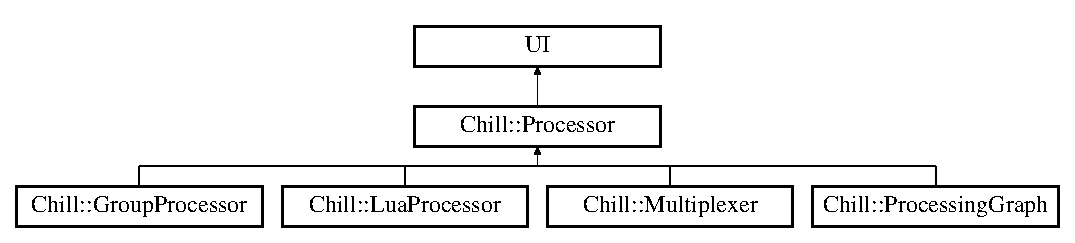
\includegraphics[height=2.818792cm]{class_chill_1_1_processor}
\end{center}
\end{figure}
\subsection*{Public Member Functions}
\begin{DoxyCompactItemize}
\item 
\mbox{\hyperlink{class_chill_1_1_processor_ae4f5d1338dcae8154ea8339cb2524fd1}{Processor}} ()
\item 
\mbox{\hyperlink{class_chill_1_1_processor_ac8ef42b4ab4e0c32265743691d4bb272}{Processor}} (const std\+::string \&\+\_\+name)
\item 
\mbox{\hyperlink{class_chill_1_1_processor_aed80279651d92dd2d3077120ba2c8491}{Processor}} (\mbox{\hyperlink{class_chill_1_1_processing_graph}{Processing\+Graph}} $\ast$\+\_\+owner)
\item 
\mbox{\hyperlink{class_chill_1_1_processor_a36d7f0ccee9cfa13fbe58cee33619521}{Processor}} (const \mbox{\hyperlink{class_chill_1_1_processor}{Processor}} \&\+\_\+copy)
\item 
const std\+::string \mbox{\hyperlink{class_chill_1_1_processor_a8d35027206ef53bd40d2554f2f4b9046}{name}} ()
\item 
void \mbox{\hyperlink{class_chill_1_1_processor_a1daa8b6fe879d65d96ca507a64a2adf0}{set\+Name}} (std\+::string \+\_\+name)
\item 
Im\+U32 \mbox{\hyperlink{class_chill_1_1_processor_a4ee8538c5b95c44cd04224efd86f94bf}{get\+Color}} ()
\item 
void \mbox{\hyperlink{class_chill_1_1_processor_ae0835b5fa85f9038911a72b2c293b7b3}{set\+Color}} (const Im\+U32 \&\+\_\+color)
\item 
void \mbox{\hyperlink{class_chill_1_1_processor_a295fa343c9c834d8c29f057aa0754d30}{set\+Owner}} (\mbox{\hyperlink{class_chill_1_1_processing_graph}{Processing\+Graph}} $\ast$\+\_\+owner)
\item 
\mbox{\hyperlink{class_chill_1_1_processing_graph}{Processing\+Graph}} $\ast$ \mbox{\hyperlink{class_chill_1_1_processor_a3024af1d7f7785b03485a79eece5be3b}{owner}} ()
\item 
const std\+::vector$<$ Auto\+Ptr$<$ \mbox{\hyperlink{class_chill_1_1_processor_input}{Processor\+Input}} $>$ $>$ \mbox{\hyperlink{class_chill_1_1_processor_ae31251f77eaca1c86fb326cac6833695}{inputs}} ()
\item 
std\+::vector$<$ Auto\+Ptr$<$ \mbox{\hyperlink{class_chill_1_1_processor_output}{Processor\+Output}} $>$ $>$ \mbox{\hyperlink{class_chill_1_1_processor_a5ed85c9d070167d489eb51022863887a}{outputs}} ()
\item 
Auto\+Ptr$<$ \mbox{\hyperlink{class_chill_1_1_processor_input}{Processor\+Input}} $>$ \mbox{\hyperlink{class_chill_1_1_processor_af7e4fd8473b311ac572825193331d1e6}{input}} (std\+::string \+\_\+name)
\item 
Auto\+Ptr$<$ \mbox{\hyperlink{class_chill_1_1_processor_output}{Processor\+Output}} $>$ \mbox{\hyperlink{class_chill_1_1_processor_a26494f059d01af50bd66462e8c14fdb9}{output}} (std\+::string \+\_\+name)
\item 
Auto\+Ptr$<$ \mbox{\hyperlink{class_chill_1_1_processor_input}{Processor\+Input}} $>$ \mbox{\hyperlink{class_chill_1_1_processor_a771c81e8f921566a6ee719845c2f1e23}{add\+Input}} (Auto\+Ptr$<$ \mbox{\hyperlink{class_chill_1_1_processor_input}{Processor\+Input}} $>$ \+\_\+input)
\item 
{\footnotesize template$<$typename ... Args$>$ }\\Auto\+Ptr$<$ \mbox{\hyperlink{class_chill_1_1_processor_input}{Processor\+Input}} $>$ \mbox{\hyperlink{class_chill_1_1_processor_aa7180f4172236f0dabe725a5eabe9900}{add\+Input}} (std\+::string \+\_\+name, I\+O\+Type\+::\+I\+O\+Type \+\_\+type, Args \&\&... \+\_\+args)
\item 
Auto\+Ptr$<$ \mbox{\hyperlink{class_chill_1_1_processor_output}{Processor\+Output}} $>$ \mbox{\hyperlink{class_chill_1_1_processor_a07fdef0cf1b7c20d39739ec287ea2f87}{add\+Output}} (Auto\+Ptr$<$ \mbox{\hyperlink{class_chill_1_1_processor_output}{Processor\+Output}} $>$ \+\_\+output)
\item 
Auto\+Ptr$<$ \mbox{\hyperlink{class_chill_1_1_processor_output}{Processor\+Output}} $>$ \mbox{\hyperlink{class_chill_1_1_processor_a2bb867802937d84cb94941ebbbf43ff8}{add\+Output}} (std\+::string \+\_\+name, I\+O\+Type\+::\+I\+O\+Type \+\_\+type=I\+O\+Type\+::\+U\+N\+D\+EF)
\item 
void \mbox{\hyperlink{class_chill_1_1_processor_afff216d6d38739af754c4d6e62702214}{remove\+Input}} (Auto\+Ptr$<$ \mbox{\hyperlink{class_chill_1_1_processor_input}{Processor\+Input}} $>$ \&\+\_\+input)
\item 
void \mbox{\hyperlink{class_chill_1_1_processor_adf8c383a1b90606599e42c85f12ea7cd}{remove\+Output}} (Auto\+Ptr$<$ \mbox{\hyperlink{class_chill_1_1_processor_output}{Processor\+Output}} $>$ \&\+\_\+output)
\item 
virtual bool \mbox{\hyperlink{class_chill_1_1_processor_a2eb86d9750e1c0d5ac7f6da166aca8fd}{draw}} ()
\item 
virtual Auto\+Ptr$<$ \mbox{\hyperlink{class_chill_1_1_processor}{Processor}} $>$ \mbox{\hyperlink{class_chill_1_1_processor_ad3cc90a592d8755afb546e9b701489e4}{Processor\+::clone}} ()
\item 
virtual void \mbox{\hyperlink{class_chill_1_1_processor_a476a6eddddef2f44827e4d9de530d706}{save}} (std\+::ofstream \&\+\_\+stream)
\item 
virtual bool \mbox{\hyperlink{class_chill_1_1_processor_a209a0c41fc704874da8c2c10371d1b79}{is\+Emitting}} ()
\end{DoxyCompactItemize}
\subsection*{Public Attributes}
\begin{DoxyCompactItemize}
\item 
\mbox{\Hypertarget{class_chill_1_1_processor_a948bfa8f4cfd3112f3da8b2ffa36bb7a}\label{class_chill_1_1_processor_a948bfa8f4cfd3112f3da8b2ffa36bb7a}} 
char {\bfseries m\+\_\+title} \mbox{[}32\mbox{]} = \char`\"{}\textbackslash{}0\char`\"{}
\item 
\mbox{\Hypertarget{class_chill_1_1_processor_abcba3bd72b99bbaeed8c715e0772fbda}\label{class_chill_1_1_processor_abcba3bd72b99bbaeed8c715e0772fbda}} 
bool {\bfseries m\+\_\+selected} = false
\item 
\mbox{\Hypertarget{class_chill_1_1_processor_ac82c72fce70c6b897c7fb61ec6108fc7}\label{class_chill_1_1_processor_ac82c72fce70c6b897c7fb61ec6108fc7}} 
bool {\bfseries m\+\_\+edit} = false
\end{DoxyCompactItemize}
\subsection*{Protected Attributes}
\begin{DoxyCompactItemize}
\item 
std\+::string \mbox{\hyperlink{class_chill_1_1_processor_aa6a9be29fed9833aef0c75259653bd20}{m\+\_\+name}}
\item 
Im\+U32 \mbox{\hyperlink{class_chill_1_1_processor_ae473cb6e402c7454ed4225c70da8de6c}{m\+\_\+color}}
\item 
\mbox{\hyperlink{class_chill_1_1_processing_graph}{Processing\+Graph}} $\ast$ \mbox{\hyperlink{class_chill_1_1_processor_a2b83d506f9923cb479d553f90acd2a02}{m\+\_\+owner}}
\item 
bool \mbox{\hyperlink{class_chill_1_1_processor_afbe48b147ae854cca4b93dfb3e5f0e8a}{m\+\_\+emit}} = false
\item 
std\+::vector$<$ Auto\+Ptr$<$ \mbox{\hyperlink{class_chill_1_1_processor_input}{Processor\+Input}} $>$ $>$ \mbox{\hyperlink{class_chill_1_1_processor_a9843bceefbc8f8236f0e7a05427378c1}{m\+\_\+inputs}}
\item 
std\+::vector$<$ Auto\+Ptr$<$ \mbox{\hyperlink{class_chill_1_1_processor_output}{Processor\+Output}} $>$ $>$ \mbox{\hyperlink{class_chill_1_1_processor_a0d0fdbd5faed69b8293b7cd615d96f99}{m\+\_\+outputs}}
\end{DoxyCompactItemize}


\subsection{Detailed Description}
\mbox{\hyperlink{class_chill_1_1_processor}{Processor}} class. Is a node within the graph. Contains inputs and outputs. 

\subsection{Constructor \& Destructor Documentation}
\mbox{\Hypertarget{class_chill_1_1_processor_ae4f5d1338dcae8154ea8339cb2524fd1}\label{class_chill_1_1_processor_ae4f5d1338dcae8154ea8339cb2524fd1}} 
\index{Chill\+::\+Processor@{Chill\+::\+Processor}!Processor@{Processor}}
\index{Processor@{Processor}!Chill\+::\+Processor@{Chill\+::\+Processor}}
\subsubsection{\texorpdfstring{Processor()}{Processor()}\hspace{0.1cm}{\footnotesize\ttfamily [1/4]}}
{\footnotesize\ttfamily Chill\+::\+Processor\+::\+Processor (\begin{DoxyParamCaption}{ }\end{DoxyParamCaption})\hspace{0.3cm}{\ttfamily [inline]}}

Instanciate a new \mbox{\hyperlink{class_chill_1_1_processor}{Processor}}. \mbox{\Hypertarget{class_chill_1_1_processor_ac8ef42b4ab4e0c32265743691d4bb272}\label{class_chill_1_1_processor_ac8ef42b4ab4e0c32265743691d4bb272}} 
\index{Chill\+::\+Processor@{Chill\+::\+Processor}!Processor@{Processor}}
\index{Processor@{Processor}!Chill\+::\+Processor@{Chill\+::\+Processor}}
\subsubsection{\texorpdfstring{Processor()}{Processor()}\hspace{0.1cm}{\footnotesize\ttfamily [2/4]}}
{\footnotesize\ttfamily Chill\+::\+Processor\+::\+Processor (\begin{DoxyParamCaption}\item[{const std\+::string \&}]{\+\_\+name }\end{DoxyParamCaption})\hspace{0.3cm}{\ttfamily [inline]}}

Instanciate a new \mbox{\hyperlink{class_chill_1_1_processor}{Processor}}. 
\begin{DoxyParams}{Parameters}
{\em \+\_\+name} & The name of the processor \\
\hline
\end{DoxyParams}
\mbox{\Hypertarget{class_chill_1_1_processor_aed80279651d92dd2d3077120ba2c8491}\label{class_chill_1_1_processor_aed80279651d92dd2d3077120ba2c8491}} 
\index{Chill\+::\+Processor@{Chill\+::\+Processor}!Processor@{Processor}}
\index{Processor@{Processor}!Chill\+::\+Processor@{Chill\+::\+Processor}}
\subsubsection{\texorpdfstring{Processor()}{Processor()}\hspace{0.1cm}{\footnotesize\ttfamily [3/4]}}
{\footnotesize\ttfamily Chill\+::\+Processor\+::\+Processor (\begin{DoxyParamCaption}\item[{\mbox{\hyperlink{class_chill_1_1_processing_graph}{Processing\+Graph}} $\ast$}]{\+\_\+owner }\end{DoxyParamCaption})\hspace{0.3cm}{\ttfamily [inline]}}

Instanciate a new \mbox{\hyperlink{class_chill_1_1_processor}{Processor}} and set is owner. 
\begin{DoxyParams}{Parameters}
{\em \+\_\+owner} & Parent graph that contains the processor. \\
\hline
\end{DoxyParams}
\mbox{\Hypertarget{class_chill_1_1_processor_a36d7f0ccee9cfa13fbe58cee33619521}\label{class_chill_1_1_processor_a36d7f0ccee9cfa13fbe58cee33619521}} 
\index{Chill\+::\+Processor@{Chill\+::\+Processor}!Processor@{Processor}}
\index{Processor@{Processor}!Chill\+::\+Processor@{Chill\+::\+Processor}}
\subsubsection{\texorpdfstring{Processor()}{Processor()}\hspace{0.1cm}{\footnotesize\ttfamily [4/4]}}
{\footnotesize\ttfamily Chill\+::\+Processor\+::\+Processor (\begin{DoxyParamCaption}\item[{const \mbox{\hyperlink{class_chill_1_1_processor}{Processor}} \&}]{\+\_\+copy }\end{DoxyParamCaption})}

Copy constructor. 
\begin{DoxyParams}{Parameters}
{\em \+\_\+copy} & The processor which gonna be copied. \\
\hline
\end{DoxyParams}


\subsection{Member Function Documentation}
\mbox{\Hypertarget{class_chill_1_1_processor_a771c81e8f921566a6ee719845c2f1e23}\label{class_chill_1_1_processor_a771c81e8f921566a6ee719845c2f1e23}} 
\index{Chill\+::\+Processor@{Chill\+::\+Processor}!add\+Input@{add\+Input}}
\index{add\+Input@{add\+Input}!Chill\+::\+Processor@{Chill\+::\+Processor}}
\subsubsection{\texorpdfstring{add\+Input()}{addInput()}\hspace{0.1cm}{\footnotesize\ttfamily [1/2]}}
{\footnotesize\ttfamily Auto\+Ptr$<$ \mbox{\hyperlink{class_chill_1_1_processor_input}{Processor\+Input}} $>$ Chill\+::\+Processor\+::add\+Input (\begin{DoxyParamCaption}\item[{Auto\+Ptr$<$ \mbox{\hyperlink{class_chill_1_1_processor_input}{Processor\+Input}} $>$}]{\+\_\+input }\end{DoxyParamCaption})}

Add a new input to the processor. 
\begin{DoxyParams}{Parameters}
{\em \+\_\+input} & The input. \\
\hline
\end{DoxyParams}
\begin{DoxyReturn}{Returns}
A pointer to the new input. 
\end{DoxyReturn}
\mbox{\Hypertarget{class_chill_1_1_processor_aa7180f4172236f0dabe725a5eabe9900}\label{class_chill_1_1_processor_aa7180f4172236f0dabe725a5eabe9900}} 
\index{Chill\+::\+Processor@{Chill\+::\+Processor}!add\+Input@{add\+Input}}
\index{add\+Input@{add\+Input}!Chill\+::\+Processor@{Chill\+::\+Processor}}
\subsubsection{\texorpdfstring{add\+Input()}{addInput()}\hspace{0.1cm}{\footnotesize\ttfamily [2/2]}}
{\footnotesize\ttfamily template$<$typename ... Args$>$ \\
Auto\+Ptr$<$ \mbox{\hyperlink{class_chill_1_1_processor_input}{Processor\+Input}} $>$ Chill\+::\+Processor\+::add\+Input (\begin{DoxyParamCaption}\item[{std\+::string}]{\+\_\+name,  }\item[{I\+O\+Type\+::\+I\+O\+Type}]{\+\_\+type,  }\item[{Args \&\&...}]{\+\_\+args }\end{DoxyParamCaption})}

Add a new input to the processor. 
\begin{DoxyParams}{Parameters}
{\em \+\_\+name} & The input name. \\
\hline
{\em \+\_\+type} & The input type. \\
\hline
{\em \+\_\+args} & All additionnal arguments \\
\hline
\end{DoxyParams}
\begin{DoxyReturn}{Returns}
A pointer to the new input. 
\end{DoxyReturn}
\mbox{\Hypertarget{class_chill_1_1_processor_a07fdef0cf1b7c20d39739ec287ea2f87}\label{class_chill_1_1_processor_a07fdef0cf1b7c20d39739ec287ea2f87}} 
\index{Chill\+::\+Processor@{Chill\+::\+Processor}!add\+Output@{add\+Output}}
\index{add\+Output@{add\+Output}!Chill\+::\+Processor@{Chill\+::\+Processor}}
\subsubsection{\texorpdfstring{add\+Output()}{addOutput()}\hspace{0.1cm}{\footnotesize\ttfamily [1/2]}}
{\footnotesize\ttfamily Auto\+Ptr$<$ \mbox{\hyperlink{class_chill_1_1_processor_output}{Processor\+Output}} $>$ Chill\+::\+Processor\+::add\+Output (\begin{DoxyParamCaption}\item[{Auto\+Ptr$<$ \mbox{\hyperlink{class_chill_1_1_processor_output}{Processor\+Output}} $>$}]{\+\_\+output }\end{DoxyParamCaption})}

Add a new output to the processor. 
\begin{DoxyParams}{Parameters}
{\em \+\_\+output} & The output. \\
\hline
\end{DoxyParams}
\begin{DoxyReturn}{Returns}
A pointer to the new output. 
\end{DoxyReturn}
\mbox{\Hypertarget{class_chill_1_1_processor_a2bb867802937d84cb94941ebbbf43ff8}\label{class_chill_1_1_processor_a2bb867802937d84cb94941ebbbf43ff8}} 
\index{Chill\+::\+Processor@{Chill\+::\+Processor}!add\+Output@{add\+Output}}
\index{add\+Output@{add\+Output}!Chill\+::\+Processor@{Chill\+::\+Processor}}
\subsubsection{\texorpdfstring{add\+Output()}{addOutput()}\hspace{0.1cm}{\footnotesize\ttfamily [2/2]}}
{\footnotesize\ttfamily Auto\+Ptr$<$ \mbox{\hyperlink{class_chill_1_1_processor_output}{Processor\+Output}} $>$ Chill\+::\+Processor\+::add\+Output (\begin{DoxyParamCaption}\item[{std\+::string}]{\+\_\+name,  }\item[{I\+O\+Type\+::\+I\+O\+Type}]{\+\_\+type = {\ttfamily IOType\+:\+:UNDEF} }\end{DoxyParamCaption})}

Add a new output to the processor. 
\begin{DoxyParams}{Parameters}
{\em \+\_\+name} & The output name. \\
\hline
{\em \+\_\+type} & The output type. \\
\hline
\end{DoxyParams}
\begin{DoxyReturn}{Returns}
A pointer to the new output. 
\end{DoxyReturn}
\mbox{\Hypertarget{class_chill_1_1_processor_a2eb86d9750e1c0d5ac7f6da166aca8fd}\label{class_chill_1_1_processor_a2eb86d9750e1c0d5ac7f6da166aca8fd}} 
\index{Chill\+::\+Processor@{Chill\+::\+Processor}!draw@{draw}}
\index{draw@{draw}!Chill\+::\+Processor@{Chill\+::\+Processor}}
\subsubsection{\texorpdfstring{draw()}{draw()}}
{\footnotesize\ttfamily bool Chill\+::\+Processor\+::draw (\begin{DoxyParamCaption}{ }\end{DoxyParamCaption})\hspace{0.3cm}{\ttfamily [virtual]}}

Draw the processor 

Implements \mbox{\hyperlink{class_u_i_a5025b88e26f21852c0cd2e4b42675c50}{UI}}.



Reimplemented in \mbox{\hyperlink{class_chill_1_1_multiplexer_aac8cf52a617091ffedaee970b5550270}{Chill\+::\+Multiplexer}}, and \mbox{\hyperlink{class_chill_1_1_group_processor_a6c3eadfcb171c48a2d76bebefd153fcb}{Chill\+::\+Group\+Processor}}.

\mbox{\Hypertarget{class_chill_1_1_processor_a4ee8538c5b95c44cd04224efd86f94bf}\label{class_chill_1_1_processor_a4ee8538c5b95c44cd04224efd86f94bf}} 
\index{Chill\+::\+Processor@{Chill\+::\+Processor}!get\+Color@{get\+Color}}
\index{get\+Color@{get\+Color}!Chill\+::\+Processor@{Chill\+::\+Processor}}
\subsubsection{\texorpdfstring{get\+Color()}{getColor()}}
{\footnotesize\ttfamily Im\+U32 Chill\+::\+Processor\+::get\+Color (\begin{DoxyParamCaption}{ }\end{DoxyParamCaption})\hspace{0.3cm}{\ttfamily [inline]}}

Get the color of this processor. \begin{DoxyReturn}{Returns}
The color of the processor. 
\end{DoxyReturn}
\mbox{\Hypertarget{class_chill_1_1_processor_af7e4fd8473b311ac572825193331d1e6}\label{class_chill_1_1_processor_af7e4fd8473b311ac572825193331d1e6}} 
\index{Chill\+::\+Processor@{Chill\+::\+Processor}!input@{input}}
\index{input@{input}!Chill\+::\+Processor@{Chill\+::\+Processor}}
\subsubsection{\texorpdfstring{input()}{input()}}
{\footnotesize\ttfamily Auto\+Ptr$<$ \mbox{\hyperlink{class_chill_1_1_processor_input}{Processor\+Input}} $>$ Chill\+::\+Processor\+::input (\begin{DoxyParamCaption}\item[{std\+::string}]{\+\_\+name }\end{DoxyParamCaption})}

Get an input by name. 
\begin{DoxyParams}{Parameters}
{\em \+\_\+name} & The input name. \\
\hline
\end{DoxyParams}
\begin{DoxyReturn}{Returns}
The input pointer if exists else a null pointer. 
\end{DoxyReturn}
\mbox{\Hypertarget{class_chill_1_1_processor_ae31251f77eaca1c86fb326cac6833695}\label{class_chill_1_1_processor_ae31251f77eaca1c86fb326cac6833695}} 
\index{Chill\+::\+Processor@{Chill\+::\+Processor}!inputs@{inputs}}
\index{inputs@{inputs}!Chill\+::\+Processor@{Chill\+::\+Processor}}
\subsubsection{\texorpdfstring{inputs()}{inputs()}}
{\footnotesize\ttfamily const std\+::vector$<$Auto\+Ptr$<$\mbox{\hyperlink{class_chill_1_1_processor_input}{Processor\+Input}}$>$ $>$ Chill\+::\+Processor\+::inputs (\begin{DoxyParamCaption}{ }\end{DoxyParamCaption})\hspace{0.3cm}{\ttfamily [inline]}}

Get the list of inputs. \begin{DoxyReturn}{Returns}
The list of inputs. 
\end{DoxyReturn}
\mbox{\Hypertarget{class_chill_1_1_processor_a209a0c41fc704874da8c2c10371d1b79}\label{class_chill_1_1_processor_a209a0c41fc704874da8c2c10371d1b79}} 
\index{Chill\+::\+Processor@{Chill\+::\+Processor}!is\+Emitting@{is\+Emitting}}
\index{is\+Emitting@{is\+Emitting}!Chill\+::\+Processor@{Chill\+::\+Processor}}
\subsubsection{\texorpdfstring{is\+Emitting()}{isEmitting()}}
{\footnotesize\ttfamily bool Chill\+::\+Processor\+::is\+Emitting (\begin{DoxyParamCaption}{ }\end{DoxyParamCaption})\hspace{0.3cm}{\ttfamily [virtual]}}

\begin{DoxyReturn}{Returns}
true if affects any output (shape or slicing parameter) 
\end{DoxyReturn}
\mbox{\Hypertarget{class_chill_1_1_processor_a8d35027206ef53bd40d2554f2f4b9046}\label{class_chill_1_1_processor_a8d35027206ef53bd40d2554f2f4b9046}} 
\index{Chill\+::\+Processor@{Chill\+::\+Processor}!name@{name}}
\index{name@{name}!Chill\+::\+Processor@{Chill\+::\+Processor}}
\subsubsection{\texorpdfstring{name()}{name()}}
{\footnotesize\ttfamily const std\+::string Chill\+::\+Processor\+::name (\begin{DoxyParamCaption}{ }\end{DoxyParamCaption})\hspace{0.3cm}{\ttfamily [inline]}}

Get the name of this processor. \begin{DoxyReturn}{Returns}
The name of the processor. 
\end{DoxyReturn}
\mbox{\Hypertarget{class_chill_1_1_processor_a26494f059d01af50bd66462e8c14fdb9}\label{class_chill_1_1_processor_a26494f059d01af50bd66462e8c14fdb9}} 
\index{Chill\+::\+Processor@{Chill\+::\+Processor}!output@{output}}
\index{output@{output}!Chill\+::\+Processor@{Chill\+::\+Processor}}
\subsubsection{\texorpdfstring{output()}{output()}}
{\footnotesize\ttfamily Auto\+Ptr$<$ \mbox{\hyperlink{class_chill_1_1_processor_output}{Processor\+Output}} $>$ Chill\+::\+Processor\+::output (\begin{DoxyParamCaption}\item[{std\+::string}]{\+\_\+name }\end{DoxyParamCaption})}

Get an output by name. 
\begin{DoxyParams}{Parameters}
{\em \+\_\+name} & The output name. \\
\hline
\end{DoxyParams}
\begin{DoxyReturn}{Returns}
The output pointer if exists else a null pointer. 
\end{DoxyReturn}
\mbox{\Hypertarget{class_chill_1_1_processor_a5ed85c9d070167d489eb51022863887a}\label{class_chill_1_1_processor_a5ed85c9d070167d489eb51022863887a}} 
\index{Chill\+::\+Processor@{Chill\+::\+Processor}!outputs@{outputs}}
\index{outputs@{outputs}!Chill\+::\+Processor@{Chill\+::\+Processor}}
\subsubsection{\texorpdfstring{outputs()}{outputs()}}
{\footnotesize\ttfamily std\+::vector$<$Auto\+Ptr$<$\mbox{\hyperlink{class_chill_1_1_processor_output}{Processor\+Output}}$>$ $>$ Chill\+::\+Processor\+::outputs (\begin{DoxyParamCaption}{ }\end{DoxyParamCaption})\hspace{0.3cm}{\ttfamily [inline]}}

Get the list of outputs. \begin{DoxyReturn}{Returns}
The list of outputs. 
\end{DoxyReturn}
\mbox{\Hypertarget{class_chill_1_1_processor_a3024af1d7f7785b03485a79eece5be3b}\label{class_chill_1_1_processor_a3024af1d7f7785b03485a79eece5be3b}} 
\index{Chill\+::\+Processor@{Chill\+::\+Processor}!owner@{owner}}
\index{owner@{owner}!Chill\+::\+Processor@{Chill\+::\+Processor}}
\subsubsection{\texorpdfstring{owner()}{owner()}}
{\footnotesize\ttfamily \mbox{\hyperlink{class_chill_1_1_processing_graph}{Processing\+Graph}}$\ast$ Chill\+::\+Processor\+::owner (\begin{DoxyParamCaption}{ }\end{DoxyParamCaption})\hspace{0.3cm}{\ttfamily [inline]}}

Get the owner of this processor. \begin{DoxyReturn}{Returns}
The parent graph. 
\end{DoxyReturn}
\mbox{\Hypertarget{class_chill_1_1_processor_ad3cc90a592d8755afb546e9b701489e4}\label{class_chill_1_1_processor_ad3cc90a592d8755afb546e9b701489e4}} 
\index{Chill\+::\+Processor@{Chill\+::\+Processor}!Processor\+::clone@{Processor\+::clone}}
\index{Processor\+::clone@{Processor\+::clone}!Chill\+::\+Processor@{Chill\+::\+Processor}}
\subsubsection{\texorpdfstring{Processor\+::clone()}{Processor::clone()}}
{\footnotesize\ttfamily virtual Auto\+Ptr$<$\mbox{\hyperlink{class_chill_1_1_processor}{Processor}}$>$ Chill\+::\+Processor\+::\+Processor\+::clone (\begin{DoxyParamCaption}{ }\end{DoxyParamCaption})\hspace{0.3cm}{\ttfamily [inline]}, {\ttfamily [virtual]}}

Make a copy of the processor (deep copy) \mbox{\Hypertarget{class_chill_1_1_processor_afff216d6d38739af754c4d6e62702214}\label{class_chill_1_1_processor_afff216d6d38739af754c4d6e62702214}} 
\index{Chill\+::\+Processor@{Chill\+::\+Processor}!remove\+Input@{remove\+Input}}
\index{remove\+Input@{remove\+Input}!Chill\+::\+Processor@{Chill\+::\+Processor}}
\subsubsection{\texorpdfstring{remove\+Input()}{removeInput()}}
{\footnotesize\ttfamily void Chill\+::\+Processor\+::remove\+Input (\begin{DoxyParamCaption}\item[{Auto\+Ptr$<$ \mbox{\hyperlink{class_chill_1_1_processor_input}{Processor\+Input}} $>$ \&}]{\+\_\+input }\end{DoxyParamCaption})}

Remove an input. 
\begin{DoxyParams}{Parameters}
{\em \+\_\+input} & The pointer that refers to the input \\
\hline
\end{DoxyParams}
\mbox{\Hypertarget{class_chill_1_1_processor_adf8c383a1b90606599e42c85f12ea7cd}\label{class_chill_1_1_processor_adf8c383a1b90606599e42c85f12ea7cd}} 
\index{Chill\+::\+Processor@{Chill\+::\+Processor}!remove\+Output@{remove\+Output}}
\index{remove\+Output@{remove\+Output}!Chill\+::\+Processor@{Chill\+::\+Processor}}
\subsubsection{\texorpdfstring{remove\+Output()}{removeOutput()}}
{\footnotesize\ttfamily void Chill\+::\+Processor\+::remove\+Output (\begin{DoxyParamCaption}\item[{Auto\+Ptr$<$ \mbox{\hyperlink{class_chill_1_1_processor_output}{Processor\+Output}} $>$ \&}]{\+\_\+output }\end{DoxyParamCaption})}

Remove an output. 
\begin{DoxyParams}{Parameters}
{\em \+\_\+output} & The pointer that refers to the output \\
\hline
\end{DoxyParams}
\mbox{\Hypertarget{class_chill_1_1_processor_a476a6eddddef2f44827e4d9de530d706}\label{class_chill_1_1_processor_a476a6eddddef2f44827e4d9de530d706}} 
\index{Chill\+::\+Processor@{Chill\+::\+Processor}!save@{save}}
\index{save@{save}!Chill\+::\+Processor@{Chill\+::\+Processor}}
\subsubsection{\texorpdfstring{save()}{save()}}
{\footnotesize\ttfamily void Chill\+::\+Processor\+::save (\begin{DoxyParamCaption}\item[{std\+::ofstream \&}]{\+\_\+stream }\end{DoxyParamCaption})\hspace{0.3cm}{\ttfamily [virtual]}}

Generate the lua code and add it to the stream 
\begin{DoxyParams}{Parameters}
{\em \+\_\+stream} & The output stream \\
\hline
\end{DoxyParams}


Reimplemented in \mbox{\hyperlink{class_chill_1_1_processing_graph_a15ebc74e61a5bbdba8715c8d93b2815d}{Chill\+::\+Processing\+Graph}}.

\mbox{\Hypertarget{class_chill_1_1_processor_ae0835b5fa85f9038911a72b2c293b7b3}\label{class_chill_1_1_processor_ae0835b5fa85f9038911a72b2c293b7b3}} 
\index{Chill\+::\+Processor@{Chill\+::\+Processor}!set\+Color@{set\+Color}}
\index{set\+Color@{set\+Color}!Chill\+::\+Processor@{Chill\+::\+Processor}}
\subsubsection{\texorpdfstring{set\+Color()}{setColor()}}
{\footnotesize\ttfamily void Chill\+::\+Processor\+::set\+Color (\begin{DoxyParamCaption}\item[{const Im\+U32 \&}]{\+\_\+color }\end{DoxyParamCaption})\hspace{0.3cm}{\ttfamily [inline]}}

Set the color of this processor. 
\begin{DoxyParams}{Parameters}
{\em \+\_\+color} & The color of the processor. \\
\hline
\end{DoxyParams}
\mbox{\Hypertarget{class_chill_1_1_processor_a1daa8b6fe879d65d96ca507a64a2adf0}\label{class_chill_1_1_processor_a1daa8b6fe879d65d96ca507a64a2adf0}} 
\index{Chill\+::\+Processor@{Chill\+::\+Processor}!set\+Name@{set\+Name}}
\index{set\+Name@{set\+Name}!Chill\+::\+Processor@{Chill\+::\+Processor}}
\subsubsection{\texorpdfstring{set\+Name()}{setName()}}
{\footnotesize\ttfamily void Chill\+::\+Processor\+::set\+Name (\begin{DoxyParamCaption}\item[{std\+::string}]{\+\_\+name }\end{DoxyParamCaption})\hspace{0.3cm}{\ttfamily [inline]}}

Set the name of this processor. 
\begin{DoxyParams}{Parameters}
{\em \+\_\+name} & The name of the processor. \\
\hline
\end{DoxyParams}
\mbox{\Hypertarget{class_chill_1_1_processor_a295fa343c9c834d8c29f057aa0754d30}\label{class_chill_1_1_processor_a295fa343c9c834d8c29f057aa0754d30}} 
\index{Chill\+::\+Processor@{Chill\+::\+Processor}!set\+Owner@{set\+Owner}}
\index{set\+Owner@{set\+Owner}!Chill\+::\+Processor@{Chill\+::\+Processor}}
\subsubsection{\texorpdfstring{set\+Owner()}{setOwner()}}
{\footnotesize\ttfamily void Chill\+::\+Processor\+::set\+Owner (\begin{DoxyParamCaption}\item[{\mbox{\hyperlink{class_chill_1_1_processing_graph}{Processing\+Graph}} $\ast$}]{\+\_\+owner }\end{DoxyParamCaption})\hspace{0.3cm}{\ttfamily [inline]}}

Set a new owner. 
\begin{DoxyParams}{Parameters}
{\em \+\_\+owner} & The graph that contains this processor. \\
\hline
\end{DoxyParams}


\subsection{Member Data Documentation}
\mbox{\Hypertarget{class_chill_1_1_processor_ae473cb6e402c7454ed4225c70da8de6c}\label{class_chill_1_1_processor_ae473cb6e402c7454ed4225c70da8de6c}} 
\index{Chill\+::\+Processor@{Chill\+::\+Processor}!m\+\_\+color@{m\+\_\+color}}
\index{m\+\_\+color@{m\+\_\+color}!Chill\+::\+Processor@{Chill\+::\+Processor}}
\subsubsection{\texorpdfstring{m\+\_\+color}{m\_color}}
{\footnotesize\ttfamily Im\+U32 Chill\+::\+Processor\+::m\+\_\+color\hspace{0.3cm}{\ttfamily [protected]}}

Display color. \mbox{\Hypertarget{class_chill_1_1_processor_afbe48b147ae854cca4b93dfb3e5f0e8a}\label{class_chill_1_1_processor_afbe48b147ae854cca4b93dfb3e5f0e8a}} 
\index{Chill\+::\+Processor@{Chill\+::\+Processor}!m\+\_\+emit@{m\+\_\+emit}}
\index{m\+\_\+emit@{m\+\_\+emit}!Chill\+::\+Processor@{Chill\+::\+Processor}}
\subsubsection{\texorpdfstring{m\+\_\+emit}{m\_emit}}
{\footnotesize\ttfamily bool Chill\+::\+Processor\+::m\+\_\+emit = false\hspace{0.3cm}{\ttfamily [protected]}}

Emit a shape or a slicing parameter \mbox{\Hypertarget{class_chill_1_1_processor_a9843bceefbc8f8236f0e7a05427378c1}\label{class_chill_1_1_processor_a9843bceefbc8f8236f0e7a05427378c1}} 
\index{Chill\+::\+Processor@{Chill\+::\+Processor}!m\+\_\+inputs@{m\+\_\+inputs}}
\index{m\+\_\+inputs@{m\+\_\+inputs}!Chill\+::\+Processor@{Chill\+::\+Processor}}
\subsubsection{\texorpdfstring{m\+\_\+inputs}{m\_inputs}}
{\footnotesize\ttfamily std\+::vector$<$Auto\+Ptr$<$\mbox{\hyperlink{class_chill_1_1_processor_input}{Processor\+Input}}$>$ $>$ Chill\+::\+Processor\+::m\+\_\+inputs\hspace{0.3cm}{\ttfamily [protected]}}

List of all inputs. \mbox{\Hypertarget{class_chill_1_1_processor_aa6a9be29fed9833aef0c75259653bd20}\label{class_chill_1_1_processor_aa6a9be29fed9833aef0c75259653bd20}} 
\index{Chill\+::\+Processor@{Chill\+::\+Processor}!m\+\_\+name@{m\+\_\+name}}
\index{m\+\_\+name@{m\+\_\+name}!Chill\+::\+Processor@{Chill\+::\+Processor}}
\subsubsection{\texorpdfstring{m\+\_\+name}{m\_name}}
{\footnotesize\ttfamily std\+::string Chill\+::\+Processor\+::m\+\_\+name\hspace{0.3cm}{\ttfamily [protected]}}

Display name. \mbox{\Hypertarget{class_chill_1_1_processor_a0d0fdbd5faed69b8293b7cd615d96f99}\label{class_chill_1_1_processor_a0d0fdbd5faed69b8293b7cd615d96f99}} 
\index{Chill\+::\+Processor@{Chill\+::\+Processor}!m\+\_\+outputs@{m\+\_\+outputs}}
\index{m\+\_\+outputs@{m\+\_\+outputs}!Chill\+::\+Processor@{Chill\+::\+Processor}}
\subsubsection{\texorpdfstring{m\+\_\+outputs}{m\_outputs}}
{\footnotesize\ttfamily std\+::vector$<$Auto\+Ptr$<$\mbox{\hyperlink{class_chill_1_1_processor_output}{Processor\+Output}}$>$ $>$ Chill\+::\+Processor\+::m\+\_\+outputs\hspace{0.3cm}{\ttfamily [protected]}}

List of all outputs. \mbox{\Hypertarget{class_chill_1_1_processor_a2b83d506f9923cb479d553f90acd2a02}\label{class_chill_1_1_processor_a2b83d506f9923cb479d553f90acd2a02}} 
\index{Chill\+::\+Processor@{Chill\+::\+Processor}!m\+\_\+owner@{m\+\_\+owner}}
\index{m\+\_\+owner@{m\+\_\+owner}!Chill\+::\+Processor@{Chill\+::\+Processor}}
\subsubsection{\texorpdfstring{m\+\_\+owner}{m\_owner}}
{\footnotesize\ttfamily \mbox{\hyperlink{class_chill_1_1_processing_graph}{Processing\+Graph}}$\ast$ Chill\+::\+Processor\+::m\+\_\+owner\hspace{0.3cm}{\ttfamily [protected]}}

Parent graph, raw pointer is needed. 

The documentation for this class was generated from the following files\+:\begin{DoxyCompactItemize}
\item 
E\+:/\+Chill/chill/chill\+Engine/\mbox{\hyperlink{_processor_8h}{Processor.\+h}}\item 
E\+:/\+Chill/chill/chill\+Engine/Processor.\+cpp\end{DoxyCompactItemize}

\hypertarget{class_chill_1_1_processor_input}{}\section{Chill\+:\+:Processor\+Input Class Reference}
\label{class_chill_1_1_processor_input}\index{Chill\+::\+Processor\+Input@{Chill\+::\+Processor\+Input}}


{\ttfamily \#include $<$I\+Os.\+h$>$}

Inheritance diagram for Chill\+:\+:Processor\+Input\+:\begin{figure}[H]
\begin{center}
\leavevmode
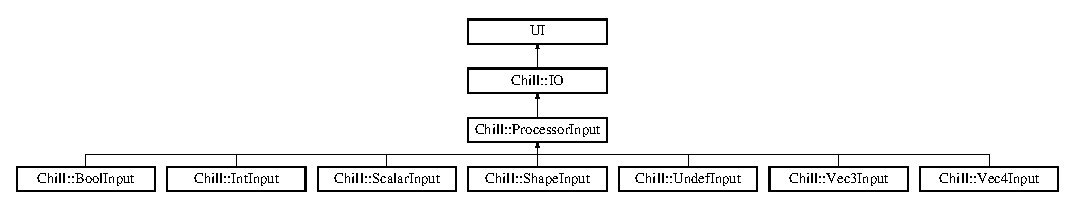
\includegraphics[height=2.352941cm]{class_chill_1_1_processor_input}
\end{center}
\end{figure}
\subsection*{Public Member Functions}
\begin{DoxyCompactItemize}
\item 
bool \mbox{\hyperlink{class_chill_1_1_processor_input_a0dfb7b669e95248d3a5974b7800aeb66}{draw}} ()
\item 
\mbox{\Hypertarget{class_chill_1_1_processor_input_ae44f1b889636b33518cdc92ee47ac3d5}\label{class_chill_1_1_processor_input_ae44f1b889636b33518cdc92ee47ac3d5}} 
virtual bool {\bfseries draw\+Tweak} ()=0
\item 
\mbox{\Hypertarget{class_chill_1_1_processor_input_afb41f8ac5e195001b6b2236701844320}\label{class_chill_1_1_processor_input_afb41f8ac5e195001b6b2236701844320}} 
virtual Auto\+Ptr$<$ \mbox{\hyperlink{class_chill_1_1_processor_input}{Processor\+Input}} $>$ {\bfseries clone} ()=0
\item 
\mbox{\Hypertarget{class_chill_1_1_processor_input_a1db7672498f9af5f0f85afa0e7889cc8}\label{class_chill_1_1_processor_input_a1db7672498f9af5f0f85afa0e7889cc8}} 
virtual void {\bfseries save} (std\+::ofstream \&\+\_\+stream)
\end{DoxyCompactItemize}
\subsection*{Static Public Member Functions}
\begin{DoxyCompactItemize}
\item 
\mbox{\Hypertarget{class_chill_1_1_processor_input_af0f82db3d6d093cbb93ab0e4eedf7bbf}\label{class_chill_1_1_processor_input_af0f82db3d6d093cbb93ab0e4eedf7bbf}} 
{\footnotesize template$<$typename... Args$>$ }\\static Auto\+Ptr$<$ \mbox{\hyperlink{class_chill_1_1_processor_input}{Processor\+Input}} $>$ {\bfseries create} (std\+::string \+\_\+name, I\+O\+Type\+::\+I\+O\+Type \+\_\+type, Args \&\&... \+\_\+args)
\end{DoxyCompactItemize}
\subsection*{Public Attributes}
\begin{DoxyCompactItemize}
\item 
Auto\+Ptr$<$ \mbox{\hyperlink{class_chill_1_1_processor_output}{Processor\+Output}} $>$ \mbox{\hyperlink{class_chill_1_1_processor_input_ab1e5cd5d0f3b9b12c3245488237177a1}{m\+\_\+link}}
\end{DoxyCompactItemize}


\subsection{Detailed Description}
Input\+Processor class. Represents a node\textquotesingle{}s input socket. 

\subsection{Member Function Documentation}
\mbox{\Hypertarget{class_chill_1_1_processor_input_a0dfb7b669e95248d3a5974b7800aeb66}\label{class_chill_1_1_processor_input_a0dfb7b669e95248d3a5974b7800aeb66}} 
\index{Chill\+::\+Processor\+Input@{Chill\+::\+Processor\+Input}!draw@{draw}}
\index{draw@{draw}!Chill\+::\+Processor\+Input@{Chill\+::\+Processor\+Input}}
\subsubsection{\texorpdfstring{draw()}{draw()}}
{\footnotesize\ttfamily bool Chill\+::\+Processor\+Input\+::draw (\begin{DoxyParamCaption}{ }\end{DoxyParamCaption})\hspace{0.3cm}{\ttfamily [virtual]}}

Draw the component return true if the element is rendered, else false 

Implements \mbox{\hyperlink{class_u_i_a5025b88e26f21852c0cd2e4b42675c50}{UI}}.



\subsection{Member Data Documentation}
\mbox{\Hypertarget{class_chill_1_1_processor_input_ab1e5cd5d0f3b9b12c3245488237177a1}\label{class_chill_1_1_processor_input_ab1e5cd5d0f3b9b12c3245488237177a1}} 
\index{Chill\+::\+Processor\+Input@{Chill\+::\+Processor\+Input}!m\+\_\+link@{m\+\_\+link}}
\index{m\+\_\+link@{m\+\_\+link}!Chill\+::\+Processor\+Input@{Chill\+::\+Processor\+Input}}
\subsubsection{\texorpdfstring{m\+\_\+link}{m\_link}}
{\footnotesize\ttfamily Auto\+Ptr$<$\mbox{\hyperlink{class_chill_1_1_processor_output}{Processor\+Output}}$>$ Chill\+::\+Processor\+Input\+::m\+\_\+link}

Linked output. 

The documentation for this class was generated from the following files\+:\begin{DoxyCompactItemize}
\item 
E\+:/\+Chill/chill/chill\+Engine/\mbox{\hyperlink{_i_os_8h}{I\+Os.\+h}}\item 
E\+:/\+Chill/chill/chill\+Engine/I\+Os.\+cpp\end{DoxyCompactItemize}

\hypertarget{class_chill_1_1_processor_output}{}\section{Chill\+:\+:Processor\+Output Class Reference}
\label{class_chill_1_1_processor_output}\index{Chill\+::\+Processor\+Output@{Chill\+::\+Processor\+Output}}


{\ttfamily \#include $<$I\+Os.\+h$>$}

Inheritance diagram for Chill\+:\+:Processor\+Output\+:\begin{figure}[H]
\begin{center}
\leavevmode
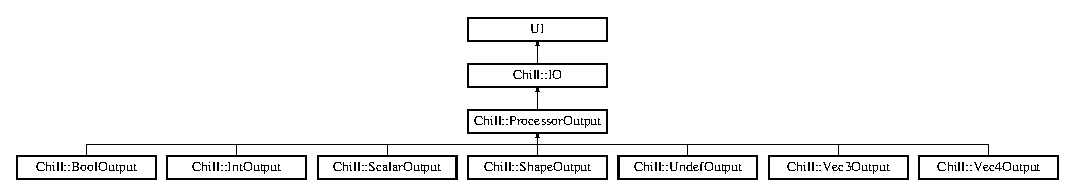
\includegraphics[height=2.191781cm]{class_chill_1_1_processor_output}
\end{center}
\end{figure}
\subsection*{Public Member Functions}
\begin{DoxyCompactItemize}
\item 
bool \mbox{\hyperlink{class_chill_1_1_processor_output_ae9d397902ac6fcd1fa09fff1cc9231c0}{draw}} ()
\item 
\mbox{\Hypertarget{class_chill_1_1_processor_output_abd2987def60f35a31eda5093f773a595}\label{class_chill_1_1_processor_output_abd2987def60f35a31eda5093f773a595}} 
virtual Auto\+Ptr$<$ \mbox{\hyperlink{class_chill_1_1_processor_output}{Processor\+Output}} $>$ {\bfseries clone} ()=0
\item 
\mbox{\Hypertarget{class_chill_1_1_processor_output_ad20a1c3db1b58a6e6b00df9c3ff44d47}\label{class_chill_1_1_processor_output_ad20a1c3db1b58a6e6b00df9c3ff44d47}} 
virtual void {\bfseries save} (std\+::ofstream \&\+\_\+stream)
\end{DoxyCompactItemize}
\subsection*{Static Public Member Functions}
\begin{DoxyCompactItemize}
\item 
\mbox{\Hypertarget{class_chill_1_1_processor_output_a41a3be6bf91145f934cdd905cc0e44c0}\label{class_chill_1_1_processor_output_a41a3be6bf91145f934cdd905cc0e44c0}} 
static Auto\+Ptr$<$ \mbox{\hyperlink{class_chill_1_1_processor_output}{Processor\+Output}} $>$ {\bfseries create} (std\+::string \+\_\+name, I\+O\+Type\+::\+I\+O\+Type \+\_\+type)
\end{DoxyCompactItemize}
\subsection*{Public Attributes}
\begin{DoxyCompactItemize}
\item 
std\+::vector$<$ Auto\+Ptr$<$ \mbox{\hyperlink{class_chill_1_1_processor_input}{Processor\+Input}} $>$ $>$ \mbox{\hyperlink{class_chill_1_1_processor_output_a538e5f1c81f00df42d8bbd6500e51dae}{m\+\_\+links}}
\end{DoxyCompactItemize}


\subsection{Detailed Description}
Output\+Processor class. Represents a node\textquotesingle{}s output socket. 

\subsection{Member Function Documentation}
\mbox{\Hypertarget{class_chill_1_1_processor_output_ae9d397902ac6fcd1fa09fff1cc9231c0}\label{class_chill_1_1_processor_output_ae9d397902ac6fcd1fa09fff1cc9231c0}} 
\index{Chill\+::\+Processor\+Output@{Chill\+::\+Processor\+Output}!draw@{draw}}
\index{draw@{draw}!Chill\+::\+Processor\+Output@{Chill\+::\+Processor\+Output}}
\subsubsection{\texorpdfstring{draw()}{draw()}}
{\footnotesize\ttfamily bool Chill\+::\+Processor\+Output\+::draw (\begin{DoxyParamCaption}{ }\end{DoxyParamCaption})\hspace{0.3cm}{\ttfamily [virtual]}}

Draw the component return true if the element is rendered, else false 

Implements \mbox{\hyperlink{class_u_i_a5025b88e26f21852c0cd2e4b42675c50}{UI}}.



\subsection{Member Data Documentation}
\mbox{\Hypertarget{class_chill_1_1_processor_output_a538e5f1c81f00df42d8bbd6500e51dae}\label{class_chill_1_1_processor_output_a538e5f1c81f00df42d8bbd6500e51dae}} 
\index{Chill\+::\+Processor\+Output@{Chill\+::\+Processor\+Output}!m\+\_\+links@{m\+\_\+links}}
\index{m\+\_\+links@{m\+\_\+links}!Chill\+::\+Processor\+Output@{Chill\+::\+Processor\+Output}}
\subsubsection{\texorpdfstring{m\+\_\+links}{m\_links}}
{\footnotesize\ttfamily std\+::vector$<$Auto\+Ptr$<$\mbox{\hyperlink{class_chill_1_1_processor_input}{Processor\+Input}}$>$ $>$ Chill\+::\+Processor\+Output\+::m\+\_\+links}

List of all linked inputs. 

The documentation for this class was generated from the following files\+:\begin{DoxyCompactItemize}
\item 
E\+:/\+Chill/chill/chill\+Engine/\mbox{\hyperlink{_i_os_8h}{I\+Os.\+h}}\item 
E\+:/\+Chill/chill/chill\+Engine/I\+Os.\+cpp\end{DoxyCompactItemize}

\hypertarget{class_chill_1_1_scalar_input}{}\section{Chill\+:\+:Scalar\+Input Class Reference}
\label{class_chill_1_1_scalar_input}\index{Chill\+::\+Scalar\+Input@{Chill\+::\+Scalar\+Input}}
Inheritance diagram for Chill\+:\+:Scalar\+Input\+:\begin{figure}[H]
\begin{center}
\leavevmode
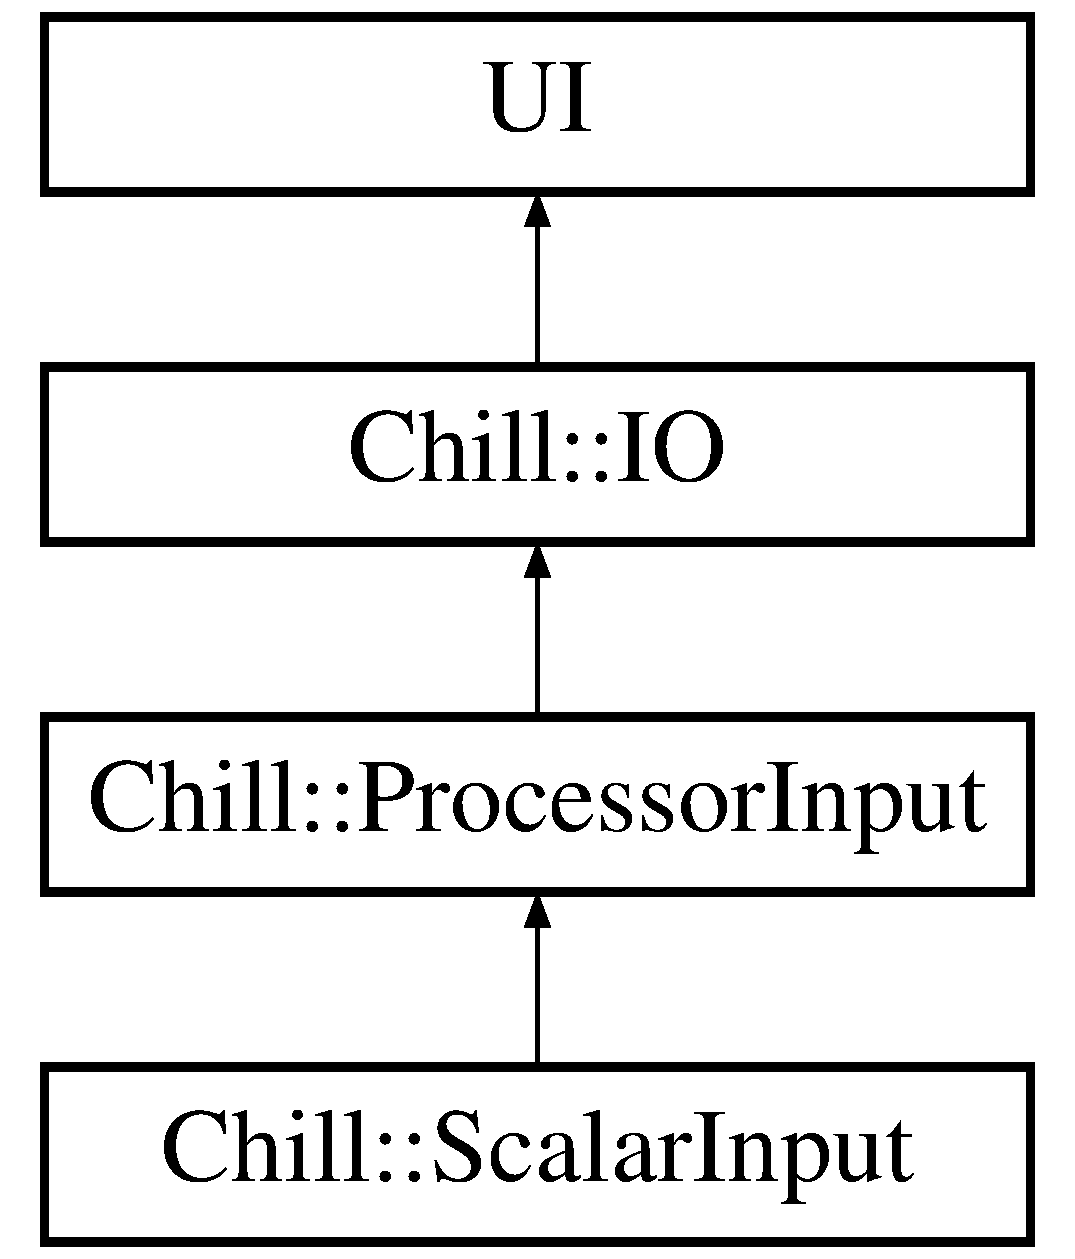
\includegraphics[height=4.000000cm]{class_chill_1_1_scalar_input}
\end{center}
\end{figure}
\subsection*{Public Member Functions}
\begin{DoxyCompactItemize}
\item 
\mbox{\Hypertarget{class_chill_1_1_scalar_input_a7d31e0df03ca9355c7e252a8273cf3cb}\label{class_chill_1_1_scalar_input_a7d31e0df03ca9355c7e252a8273cf3cb}} 
{\footnotesize template$<$typename ... Args$>$ }\\{\bfseries Scalar\+Input} (float $\ast$values\+\_\+, Args \&\&... args\+\_\+)
\item 
\mbox{\Hypertarget{class_chill_1_1_scalar_input_a42c8d6498cf139dc2c9f15cd164e7cbe}\label{class_chill_1_1_scalar_input_a42c8d6498cf139dc2c9f15cd164e7cbe}} 
{\footnotesize template$<$typename ... Args$>$ }\\{\bfseries Scalar\+Input} (float \+\_\+value=0.\+0f, float \+\_\+min=min(), float \+\_\+max=max(), bool \+\_\+slider=false, float \+\_\+step=step(), Args \&\&...)
\item 
\mbox{\Hypertarget{class_chill_1_1_scalar_input_a61d074fd513eb5a4fb60ebbf58d7e717}\label{class_chill_1_1_scalar_input_a61d074fd513eb5a4fb60ebbf58d7e717}} 
bool {\bfseries draw\+Tweak} ()
\item 
\mbox{\Hypertarget{class_chill_1_1_scalar_input_a2076ae9ebe9ac1ac6eeb789e757182b0}\label{class_chill_1_1_scalar_input_a2076ae9ebe9ac1ac6eeb789e757182b0}} 
Auto\+Ptr$<$ \mbox{\hyperlink{class_chill_1_1_processor_input}{Processor\+Input}} $>$ {\bfseries clone} ()
\item 
\mbox{\Hypertarget{class_chill_1_1_scalar_input_af5d0eb6a91d91ac043c84da0e808ea45}\label{class_chill_1_1_scalar_input_af5d0eb6a91d91ac043c84da0e808ea45}} 
void {\bfseries save} (std\+::ofstream \&\+\_\+stream)
\end{DoxyCompactItemize}
\subsection*{Static Public Member Functions}
\begin{DoxyCompactItemize}
\item 
\mbox{\Hypertarget{class_chill_1_1_scalar_input_a515f5392e0c9812016c02946962556b2}\label{class_chill_1_1_scalar_input_a515f5392e0c9812016c02946962556b2}} 
static float {\bfseries min} ()
\item 
\mbox{\Hypertarget{class_chill_1_1_scalar_input_a743cd85e03e89b7f53fc4e26c67d1f66}\label{class_chill_1_1_scalar_input_a743cd85e03e89b7f53fc4e26c67d1f66}} 
static float {\bfseries max} ()
\item 
\mbox{\Hypertarget{class_chill_1_1_scalar_input_a0520246200ea1b91d6a34a557caccdb3}\label{class_chill_1_1_scalar_input_a0520246200ea1b91d6a34a557caccdb3}} 
static float {\bfseries step} ()
\end{DoxyCompactItemize}
\subsection*{Public Attributes}
\begin{DoxyCompactItemize}
\item 
\mbox{\Hypertarget{class_chill_1_1_scalar_input_aef0a669894ff4b15e90d9b23859dcff7}\label{class_chill_1_1_scalar_input_aef0a669894ff4b15e90d9b23859dcff7}} 
float {\bfseries m\+\_\+value}
\item 
\mbox{\Hypertarget{class_chill_1_1_scalar_input_ab158a71d4b678f658a64f5bf0b9f0326}\label{class_chill_1_1_scalar_input_ab158a71d4b678f658a64f5bf0b9f0326}} 
float {\bfseries m\+\_\+min}
\item 
\mbox{\Hypertarget{class_chill_1_1_scalar_input_a187136386ed53230fd19f03af361597c}\label{class_chill_1_1_scalar_input_a187136386ed53230fd19f03af361597c}} 
float {\bfseries m\+\_\+max}
\item 
\mbox{\Hypertarget{class_chill_1_1_scalar_input_a0158b8840549aa1dc67e23d342349688}\label{class_chill_1_1_scalar_input_a0158b8840549aa1dc67e23d342349688}} 
bool {\bfseries m\+\_\+slider}
\item 
\mbox{\Hypertarget{class_chill_1_1_scalar_input_aab5578149786d972a89303ad5a9bdd6c}\label{class_chill_1_1_scalar_input_aab5578149786d972a89303ad5a9bdd6c}} 
float {\bfseries m\+\_\+step}
\end{DoxyCompactItemize}


The documentation for this class was generated from the following files\+:\begin{DoxyCompactItemize}
\item 
E\+:/\+Chill/chill/chill\+Engine/\mbox{\hyperlink{_i_os_8h}{I\+Os.\+h}}\item 
E\+:/\+Chill/chill/chill\+Engine/I\+Os.\+cpp\end{DoxyCompactItemize}

\hypertarget{class_chill_1_1_scalar_output}{}\section{Chill\+:\+:Scalar\+Output Class Reference}
\label{class_chill_1_1_scalar_output}\index{Chill\+::\+Scalar\+Output@{Chill\+::\+Scalar\+Output}}
Inheritance diagram for Chill\+:\+:Scalar\+Output\+:\begin{figure}[H]
\begin{center}
\leavevmode
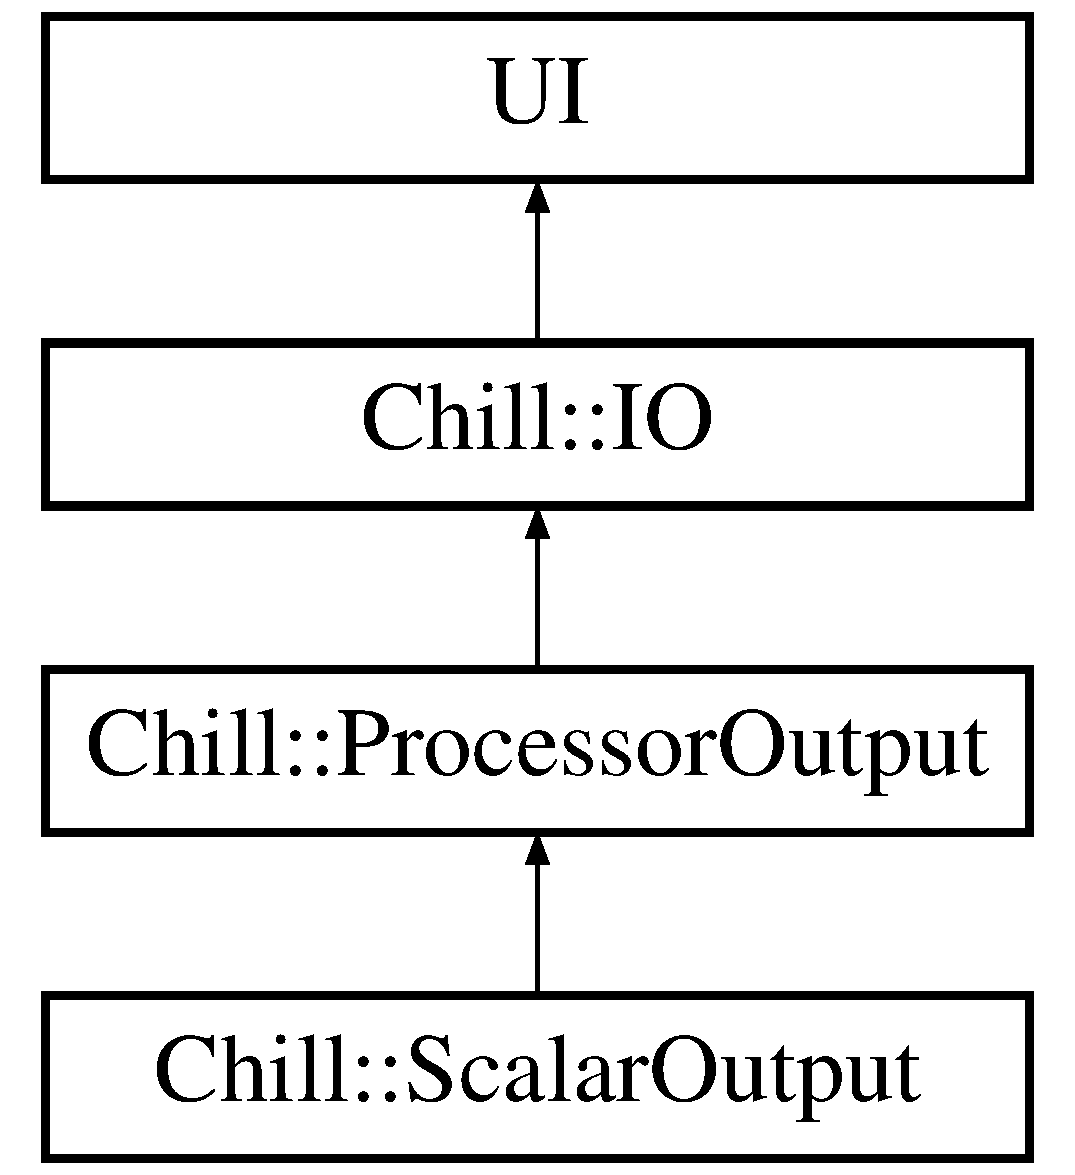
\includegraphics[height=4.000000cm]{class_chill_1_1_scalar_output}
\end{center}
\end{figure}
\subsection*{Public Member Functions}
\begin{DoxyCompactItemize}
\item 
\mbox{\Hypertarget{class_chill_1_1_scalar_output_a3e9605d5191b7299bf132ee1e423c9d2}\label{class_chill_1_1_scalar_output_a3e9605d5191b7299bf132ee1e423c9d2}} 
Auto\+Ptr$<$ \mbox{\hyperlink{class_chill_1_1_processor_output}{Processor\+Output}} $>$ {\bfseries clone} ()
\end{DoxyCompactItemize}
\subsection*{Additional Inherited Members}


The documentation for this class was generated from the following file\+:\begin{DoxyCompactItemize}
\item 
E\+:/\+Chill/chill/chill\+Engine/\mbox{\hyperlink{_i_os_8h}{I\+Os.\+h}}\end{DoxyCompactItemize}

\hypertarget{class_chill_1_1_shape_input}{}\section{Chill\+:\+:Shape\+Input Class Reference}
\label{class_chill_1_1_shape_input}\index{Chill\+::\+Shape\+Input@{Chill\+::\+Shape\+Input}}
Inheritance diagram for Chill\+:\+:Shape\+Input\+:\begin{figure}[H]
\begin{center}
\leavevmode
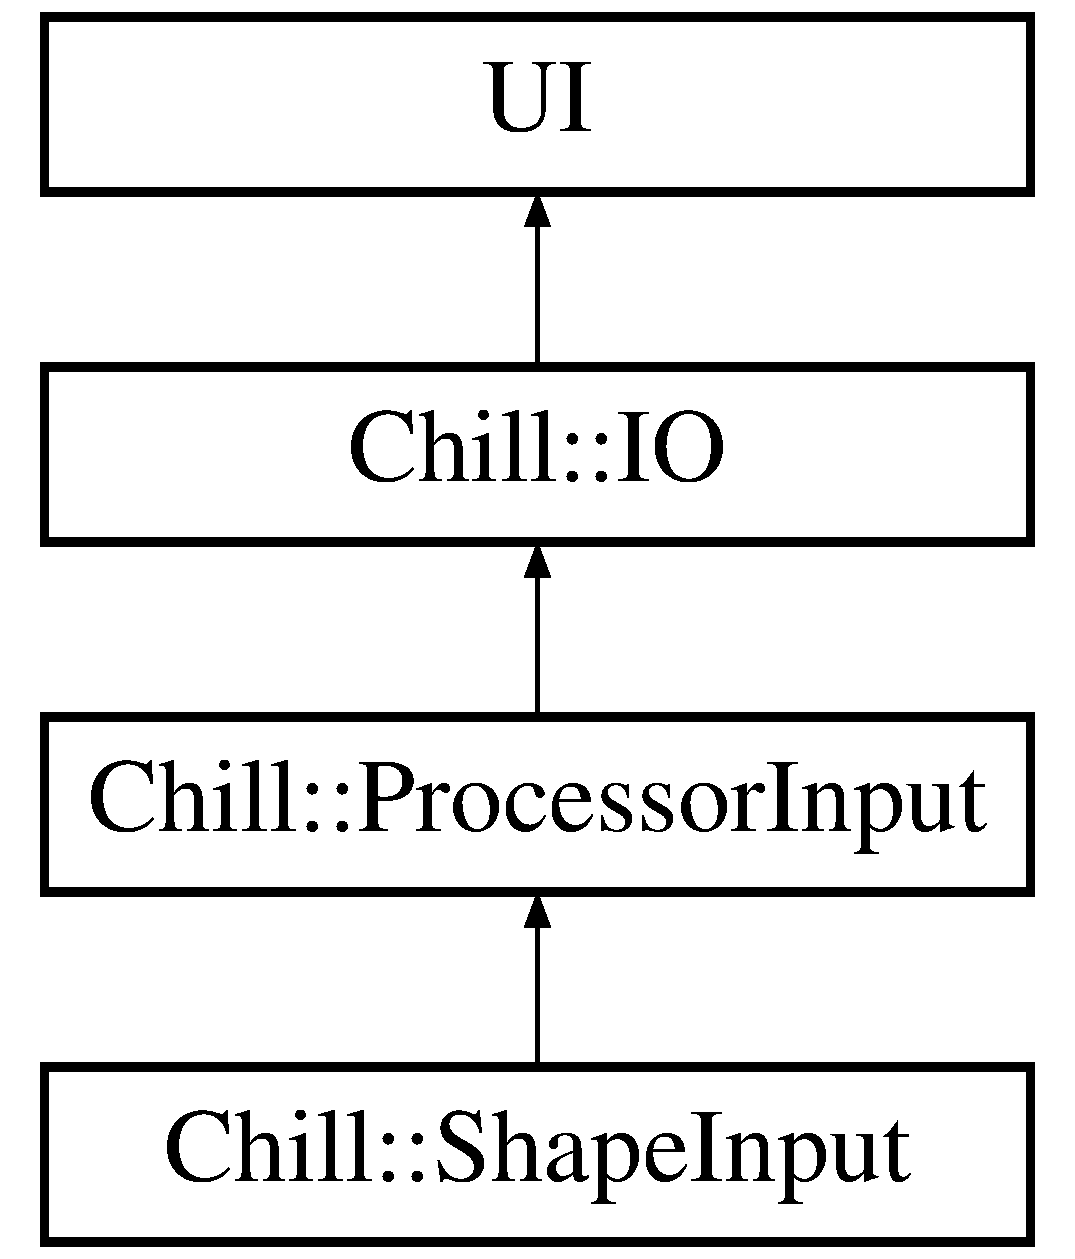
\includegraphics[height=4.000000cm]{class_chill_1_1_shape_input}
\end{center}
\end{figure}
\subsection*{Public Member Functions}
\begin{DoxyCompactItemize}
\item 
\mbox{\Hypertarget{class_chill_1_1_shape_input_a5a99471e5c5f3abca0e6964f60ca07f9}\label{class_chill_1_1_shape_input_a5a99471e5c5f3abca0e6964f60ca07f9}} 
{\footnotesize template$<$typename ... Args$>$ }\\{\bfseries Shape\+Input} (Args \&\&...)
\item 
\mbox{\Hypertarget{class_chill_1_1_shape_input_a27f594f200e3754d3961a08a3d91c598}\label{class_chill_1_1_shape_input_a27f594f200e3754d3961a08a3d91c598}} 
bool {\bfseries draw\+Tweak} ()
\item 
\mbox{\Hypertarget{class_chill_1_1_shape_input_a7f419d09fc694bdbae28dfa7293f1f46}\label{class_chill_1_1_shape_input_a7f419d09fc694bdbae28dfa7293f1f46}} 
Auto\+Ptr$<$ \mbox{\hyperlink{class_chill_1_1_processor_input}{Processor\+Input}} $>$ {\bfseries clone} ()
\item 
\mbox{\Hypertarget{class_chill_1_1_shape_input_ad5a032d3cc8f3c5674eda4369a2c3c47}\label{class_chill_1_1_shape_input_ad5a032d3cc8f3c5674eda4369a2c3c47}} 
void {\bfseries save} (std\+::ofstream \&\+\_\+stream)
\end{DoxyCompactItemize}
\subsection*{Additional Inherited Members}


The documentation for this class was generated from the following files\+:\begin{DoxyCompactItemize}
\item 
E\+:/\+Chill/chill/chill\+Engine/\mbox{\hyperlink{_i_os_8h}{I\+Os.\+h}}\item 
E\+:/\+Chill/chill/chill\+Engine/I\+Os.\+cpp\end{DoxyCompactItemize}

\hypertarget{class_chill_1_1_shape_output}{}\section{Chill\+:\+:Shape\+Output Class Reference}
\label{class_chill_1_1_shape_output}\index{Chill\+::\+Shape\+Output@{Chill\+::\+Shape\+Output}}
Inheritance diagram for Chill\+:\+:Shape\+Output\+:\begin{figure}[H]
\begin{center}
\leavevmode
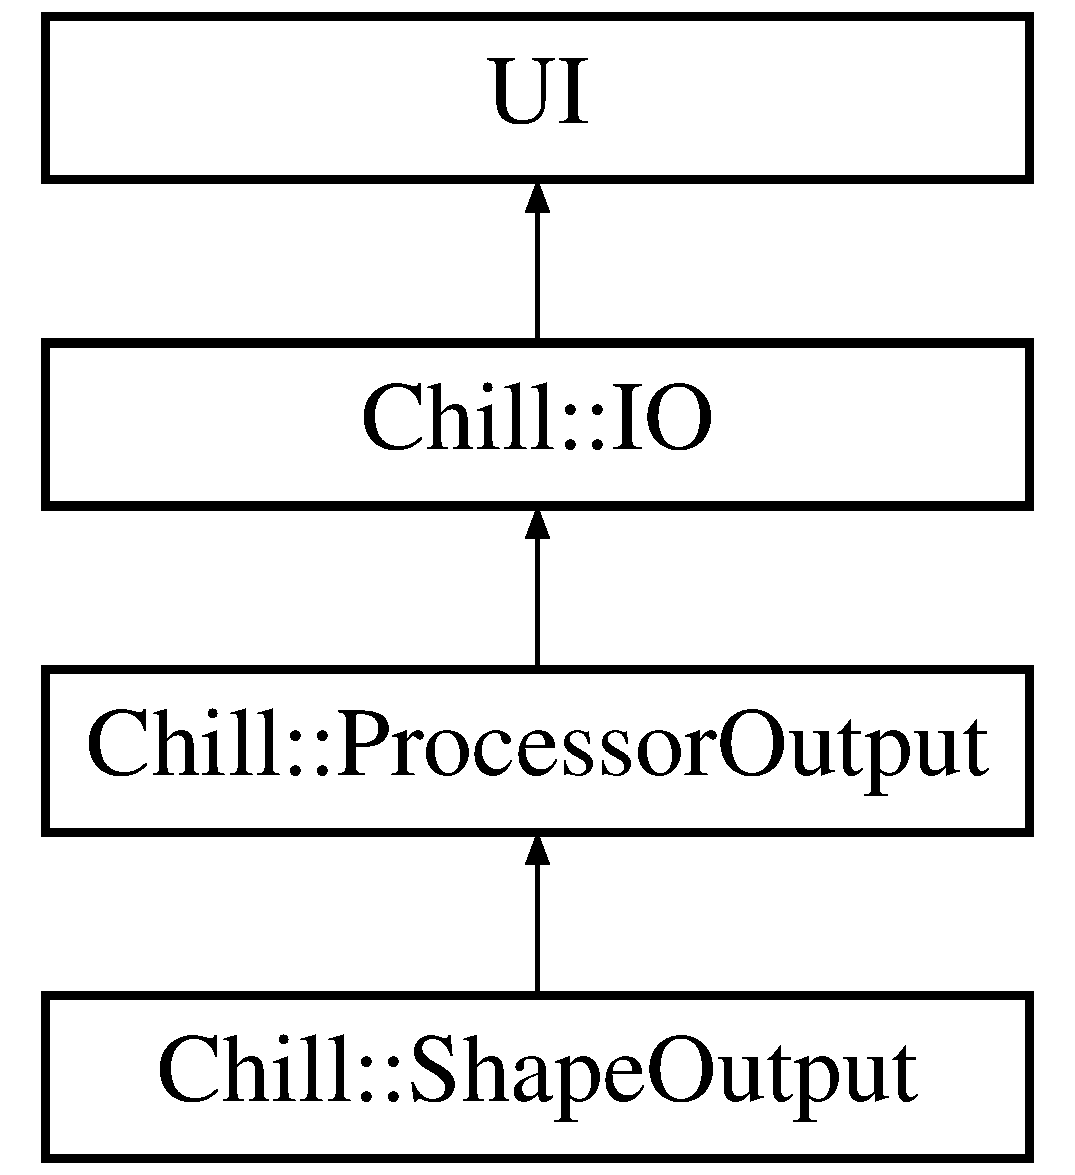
\includegraphics[height=4.000000cm]{class_chill_1_1_shape_output}
\end{center}
\end{figure}
\subsection*{Public Member Functions}
\begin{DoxyCompactItemize}
\item 
\mbox{\Hypertarget{class_chill_1_1_shape_output_a476d073fcfa8e39483253c6dd6f9dae1}\label{class_chill_1_1_shape_output_a476d073fcfa8e39483253c6dd6f9dae1}} 
Auto\+Ptr$<$ \mbox{\hyperlink{class_chill_1_1_processor_output}{Processor\+Output}} $>$ {\bfseries clone} ()
\end{DoxyCompactItemize}
\subsection*{Additional Inherited Members}


The documentation for this class was generated from the following file\+:\begin{DoxyCompactItemize}
\item 
E\+:/\+Chill/chill/chill\+Engine/\mbox{\hyperlink{_i_os_8h}{I\+Os.\+h}}\end{DoxyCompactItemize}

\hypertarget{struct_style}{}\section{Style Struct Reference}
\label{struct_style}\index{Style@{Style}}
\subsection*{Public Member Functions}
\begin{DoxyCompactItemize}
\item 
\mbox{\Hypertarget{struct_style_a0b917f3f78d79591b2ce4082e45c8186}\label{struct_style_a0b917f3f78d79591b2ce4082e45c8186}} 
Im\+Vec2 {\bfseries delta\+\_\+to\+\_\+center\+\_\+text} (Im\+Vec2 element\+\_\+size, const char $\ast$text)
\item 
\mbox{\Hypertarget{struct_style_ae4d953c69440e1a825d81bfb85a32abf}\label{struct_style_ae4d953c69440e1a825d81bfb85a32abf}} 
Im\+Vec2 {\bfseries delta\+\_\+to\+\_\+right\+\_\+text} (Im\+Vec2 element\+\_\+size, const char $\ast$text)
\end{DoxyCompactItemize}
\subsection*{Public Attributes}
\begin{DoxyCompactItemize}
\item 
\mbox{\Hypertarget{struct_style_ac3fa8abd110f98de089e832f58e8aaf0}\label{struct_style_ac3fa8abd110f98de089e832f58e8aaf0}} 
Im\+U32 {\bfseries menubar\+\_\+color}
\item 
float \mbox{\hyperlink{struct_style_a5947362709e6bf98fdbce85e79ed9e62}{menubar\+\_\+height}}
\item 
\mbox{\Hypertarget{struct_style_a902fd1c3daf51724c6be2ae352593b0d}\label{struct_style_a902fd1c3daf51724c6be2ae352593b0d}} 
Im\+U32 {\bfseries graph\+\_\+bg\+\_\+color}
\item 
\mbox{\Hypertarget{struct_style_a8f97b5a3cffeb66ead2789d6a595579d}\label{struct_style_a8f97b5a3cffeb66ead2789d6a595579d}} 
Im\+U32 {\bfseries graph\+\_\+grid\+\_\+color}
\item 
\mbox{\Hypertarget{struct_style_aec562f3e87f9ce4199390e810e3c0da5}\label{struct_style_aec562f3e87f9ce4199390e810e3c0da5}} 
float {\bfseries graph\+\_\+grid\+\_\+line\+\_\+width}
\item 
\mbox{\Hypertarget{struct_style_aa1ddff82eda0eba71e406a83418fa3fe}\label{struct_style_aa1ddff82eda0eba71e406a83418fa3fe}} 
int {\bfseries graph\+\_\+grid\+\_\+size}
\item 
\mbox{\Hypertarget{struct_style_aafd6953698a30f47e485b56a9ef209f7}\label{struct_style_aafd6953698a30f47e485b56a9ef209f7}} 
Im\+U32 {\bfseries processor\+\_\+bg\+\_\+color}
\item 
\mbox{\Hypertarget{struct_style_a7c4c4d8b4e19920b9be6fce357433b2e}\label{struct_style_a7c4c4d8b4e19920b9be6fce357433b2e}} 
Im\+U32 {\bfseries processor\+\_\+default\+\_\+color}
\item 
\mbox{\Hypertarget{struct_style_a0609e1e67a7074638a5d6dd56b34b8cb}\label{struct_style_a0609e1e67a7074638a5d6dd56b34b8cb}} 
Im\+U32 {\bfseries processor\+\_\+graph\+\_\+color}
\item 
\mbox{\Hypertarget{struct_style_ae193703063ae5a1c7ed93535a2cd5e46}\label{struct_style_ae193703063ae5a1c7ed93535a2cd5e46}} 
Im\+U32 {\bfseries processor\+\_\+group\+\_\+color}
\item 
\mbox{\Hypertarget{struct_style_a6f8f99bef171e5692fa30dc3c6a5e7ed}\label{struct_style_a6f8f99bef171e5692fa30dc3c6a5e7ed}} 
Im\+U32 {\bfseries processor\+\_\+selected\+\_\+color}
\item 
\mbox{\Hypertarget{struct_style_a8dc2b74c10a1853448e6d63c797f9dd9}\label{struct_style_a8dc2b74c10a1853448e6d63c797f9dd9}} 
Im\+U32 {\bfseries processor\+\_\+error\+\_\+color}
\item 
\mbox{\Hypertarget{struct_style_a9a2342379184911a296ddb5b5fa61f23}\label{struct_style_a9a2342379184911a296ddb5b5fa61f23}} 
Im\+U32 {\bfseries processor\+\_\+shadow\+\_\+color}
\item 
\mbox{\Hypertarget{struct_style_aef2dfe47307aa232fd6bbea1a2895815}\label{struct_style_aef2dfe47307aa232fd6bbea1a2895815}} 
Im\+U32 {\bfseries processor\+\_\+shadow\+\_\+selected\+\_\+color}
\item 
\mbox{\Hypertarget{struct_style_a2c3b2136d3815429becd92f4b7d381a2}\label{struct_style_a2c3b2136d3815429becd92f4b7d381a2}} 
Im\+U32 {\bfseries processor\+\_\+title\+\_\+bg\+\_\+color}
\item 
\mbox{\Hypertarget{struct_style_accef58fa3f882ba714f782a820bfc610}\label{struct_style_accef58fa3f882ba714f782a820bfc610}} 
Im\+U32 {\bfseries processor\+\_\+title\+\_\+color}
\item 
\mbox{\Hypertarget{struct_style_ae2f2afecfb8e8c418e8674ed3a55bfc1}\label{struct_style_ae2f2afecfb8e8c418e8674ed3a55bfc1}} 
float {\bfseries processor\+\_\+width}
\item 
\mbox{\Hypertarget{struct_style_a140f48d10f702f67364fa7e3b4eb5016}\label{struct_style_a140f48d10f702f67364fa7e3b4eb5016}} 
float {\bfseries processor\+\_\+title\+\_\+height}
\item 
\mbox{\Hypertarget{struct_style_ae092dceddfe4bfbb988bd6cd6acbcd6f}\label{struct_style_ae092dceddfe4bfbb988bd6cd6acbcd6f}} 
float {\bfseries processor\+\_\+border\+\_\+width}
\item 
\mbox{\Hypertarget{struct_style_a529777cc46850163bc1c6d9ad0f3ad07}\label{struct_style_a529777cc46850163bc1c6d9ad0f3ad07}} 
float {\bfseries processor\+\_\+rounding\+\_\+corners}
\item 
\mbox{\Hypertarget{struct_style_aee30b7b309e9a10d60227029c17fb4aa}\label{struct_style_aee30b7b309e9a10d60227029c17fb4aa}} 
int {\bfseries processor\+\_\+rounded\+\_\+corners}
\item 
\mbox{\Hypertarget{struct_style_ac7fa826d247bd87b8b5a5aaa3c57a400}\label{struct_style_ac7fa826d247bd87b8b5a5aaa3c57a400}} 
float {\bfseries socket\+\_\+radius}
\item 
\mbox{\Hypertarget{struct_style_a079f225000df13c582d14545c1cf6ae7}\label{struct_style_a079f225000df13c582d14545c1cf6ae7}} 
float {\bfseries socket\+\_\+border\+\_\+width}
\item 
\mbox{\Hypertarget{struct_style_a4355541bd6914ad241bd4462604e9625}\label{struct_style_a4355541bd6914ad241bd4462604e9625}} 
float {\bfseries min\+\_\+io\+\_\+height}
\item 
\mbox{\Hypertarget{struct_style_a287b57ed9369e4683702f862a9aaf985}\label{struct_style_a287b57ed9369e4683702f862a9aaf985}} 
Im\+Vec2 {\bfseries Item\+Spacing}
\item 
\mbox{\Hypertarget{struct_style_a3e42c2fe48f73bef052b432639edb0cf}\label{struct_style_a3e42c2fe48f73bef052b432639edb0cf}} 
Im\+U32 {\bfseries pipe\+\_\+color}
\item 
\mbox{\Hypertarget{struct_style_aa4040135b119784e3370909cadc8446b}\label{struct_style_aa4040135b119784e3370909cadc8446b}} 
Im\+U32 {\bfseries pipe\+\_\+selected\+\_\+color}
\item 
\mbox{\Hypertarget{struct_style_acc73acbaf48f7eb3e475a3a7bb1907f4}\label{struct_style_acc73acbaf48f7eb3e475a3a7bb1907f4}} 
Im\+U32 {\bfseries pipe\+\_\+error\+\_\+color}
\end{DoxyCompactItemize}


\subsection{Member Data Documentation}
\mbox{\Hypertarget{struct_style_a5947362709e6bf98fdbce85e79ed9e62}\label{struct_style_a5947362709e6bf98fdbce85e79ed9e62}} 
\index{Style@{Style}!menubar\+\_\+height@{menubar\+\_\+height}}
\index{menubar\+\_\+height@{menubar\+\_\+height}!Style@{Style}}
\subsubsection{\texorpdfstring{menubar\+\_\+height}{menubar\_height}}
{\footnotesize\ttfamily float Style\+::menubar\+\_\+height}

Height of the menu bar, needs to be updated before calling \char`\"{}\+Im\+Gui\+::\+End\+Main\+Menu\+Bar();\char`\"{} 

The documentation for this struct was generated from the following file\+:\begin{DoxyCompactItemize}
\item 
E\+:/\+Chill/chill/chill\+Engine/Style.\+h\end{DoxyCompactItemize}

\hypertarget{class_u_i}{}\section{UI Class Reference}
\label{class_u_i}\index{UI@{UI}}
Inheritance diagram for UI\+:\begin{figure}[H]
\begin{center}
\leavevmode
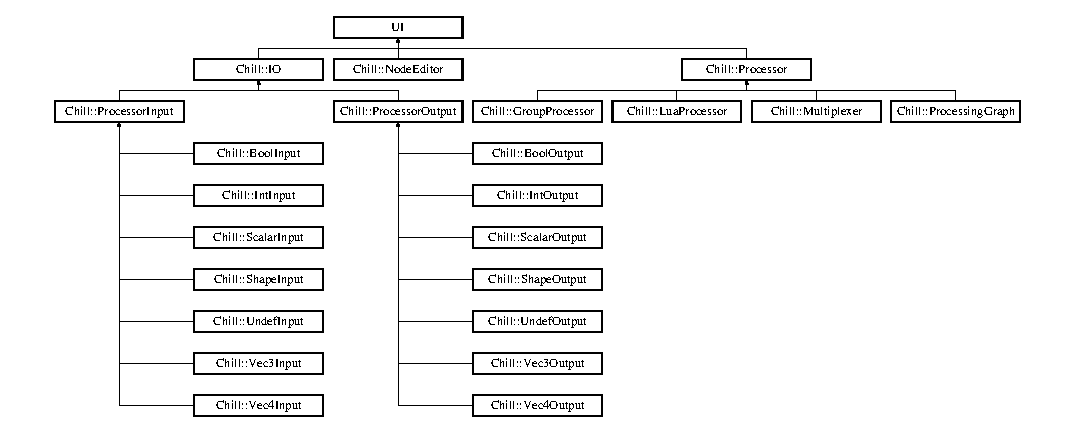
\includegraphics[height=5.369127cm]{class_u_i}
\end{center}
\end{figure}
\subsection*{Public Member Functions}
\begin{DoxyCompactItemize}
\item 
virtual bool \mbox{\hyperlink{class_u_i_a5025b88e26f21852c0cd2e4b42675c50}{draw}} ()=0
\item 
void \mbox{\hyperlink{class_u_i_a934f9deb6d5b34dfe7e510fcecab9331}{resize}} (Im\+Vec2 \+\_\+size)
\item 
void \mbox{\hyperlink{class_u_i_a3613f4288872eb4498a74929f7923144}{set\+Position}} (Im\+Vec2 \+\_\+position)
\item 
void \mbox{\hyperlink{class_u_i_a45f75304b2c3fbea67c846709a5fc3d6}{translate}} (Im\+Vec2 \+\_\+delta)
\item 
void \mbox{\hyperlink{class_u_i_a9f94b46f9c35e31475bfbf1b3d3509d4}{set\+Scale}} (const float \+\_\+scale)
\item 
\mbox{\Hypertarget{class_u_i_a5ee541a0fdace105e3a1b4ac75d09ec0}\label{class_u_i_a5ee541a0fdace105e3a1b4ac75d09ec0}} 
const Im\+Vec2 {\bfseries get\+Position} ()
\item 
\mbox{\Hypertarget{class_u_i_af2544c74b9a04087864de2a7c7915f82}\label{class_u_i_af2544c74b9a04087864de2a7c7915f82}} 
const float {\bfseries get\+Scale} ()
\item 
\mbox{\Hypertarget{class_u_i_afd4f0491687ee2c20c15c83f1faf8001}\label{class_u_i_afd4f0491687ee2c20c15c83f1faf8001}} 
const uint32\+\_\+t {\bfseries get\+Unique\+ID} ()
\end{DoxyCompactItemize}
\subsection*{Public Attributes}
\begin{DoxyCompactItemize}
\item 
\mbox{\Hypertarget{class_u_i_a168bfc22672b23e25e18c0efcbcbe21a}\label{class_u_i_a168bfc22672b23e25e18c0efcbcbe21a}} 
bool {\bfseries m\+\_\+visible} = true
\item 
Im\+Vec2 \mbox{\hyperlink{class_u_i_a15b42e4e8dfa93817e613ea089d0dfec}{m\+\_\+size}} = Im\+Vec2(0.\+0f, 0.\+0f)
\item 
Im\+Vec2 \mbox{\hyperlink{class_u_i_ad2489ec467f98fb8efa04e1724ff8bc8}{m\+\_\+position}} = Im\+Vec2(0.\+0f, 0.\+0f)
\item 
float \mbox{\hyperlink{class_u_i_a9a7264d8fcbead94498e2723204f0b63}{m\+\_\+scale}} = 1.\+0f
\item 
\mbox{\Hypertarget{class_u_i_acaab3c70fde81efa27ef2d7aa41a8f63}\label{class_u_i_acaab3c70fde81efa27ef2d7aa41a8f63}} 
\mbox{\hyperlink{struct_style}{Style}} {\bfseries style}
\end{DoxyCompactItemize}


\subsection{Member Function Documentation}
\mbox{\Hypertarget{class_u_i_a5025b88e26f21852c0cd2e4b42675c50}\label{class_u_i_a5025b88e26f21852c0cd2e4b42675c50}} 
\index{UI@{UI}!draw@{draw}}
\index{draw@{draw}!UI@{UI}}
\subsubsection{\texorpdfstring{draw()}{draw()}}
{\footnotesize\ttfamily virtual bool U\+I\+::draw (\begin{DoxyParamCaption}{ }\end{DoxyParamCaption})\hspace{0.3cm}{\ttfamily [pure virtual]}}

Draw the component return true if the element is rendered, else false 

Implemented in \mbox{\hyperlink{class_chill_1_1_multiplexer_aac8cf52a617091ffedaee970b5550270}{Chill\+::\+Multiplexer}}, \mbox{\hyperlink{class_chill_1_1_group_processor_a6c3eadfcb171c48a2d76bebefd153fcb}{Chill\+::\+Group\+Processor}}, \mbox{\hyperlink{class_chill_1_1_processor_a2eb86d9750e1c0d5ac7f6da166aca8fd}{Chill\+::\+Processor}}, \mbox{\hyperlink{class_chill_1_1_processor_input_a0dfb7b669e95248d3a5974b7800aeb66}{Chill\+::\+Processor\+Input}}, \mbox{\hyperlink{class_chill_1_1_node_editor_a7b67d5473c93d3258a2dc565e76da024}{Chill\+::\+Node\+Editor}}, and \mbox{\hyperlink{class_chill_1_1_processor_output_ae9d397902ac6fcd1fa09fff1cc9231c0}{Chill\+::\+Processor\+Output}}.

\mbox{\Hypertarget{class_u_i_a934f9deb6d5b34dfe7e510fcecab9331}\label{class_u_i_a934f9deb6d5b34dfe7e510fcecab9331}} 
\index{UI@{UI}!resize@{resize}}
\index{resize@{resize}!UI@{UI}}
\subsubsection{\texorpdfstring{resize()}{resize()}}
{\footnotesize\ttfamily void U\+I\+::resize (\begin{DoxyParamCaption}\item[{Im\+Vec2}]{\+\_\+size }\end{DoxyParamCaption})\hspace{0.3cm}{\ttfamily [inline]}}

Resize a component (scale independant) 
\begin{DoxyParams}{Parameters}
{\em \+\_\+size} & The new component size \\
\hline
\end{DoxyParams}
\mbox{\Hypertarget{class_u_i_a3613f4288872eb4498a74929f7923144}\label{class_u_i_a3613f4288872eb4498a74929f7923144}} 
\index{UI@{UI}!set\+Position@{set\+Position}}
\index{set\+Position@{set\+Position}!UI@{UI}}
\subsubsection{\texorpdfstring{set\+Position()}{setPosition()}}
{\footnotesize\ttfamily void U\+I\+::set\+Position (\begin{DoxyParamCaption}\item[{Im\+Vec2}]{\+\_\+position }\end{DoxyParamCaption})\hspace{0.3cm}{\ttfamily [inline]}}

Move a component 
\begin{DoxyParams}{Parameters}
{\em \+\_\+position} & The new position \\
\hline
\end{DoxyParams}
\mbox{\Hypertarget{class_u_i_a9f94b46f9c35e31475bfbf1b3d3509d4}\label{class_u_i_a9f94b46f9c35e31475bfbf1b3d3509d4}} 
\index{UI@{UI}!set\+Scale@{set\+Scale}}
\index{set\+Scale@{set\+Scale}!UI@{UI}}
\subsubsection{\texorpdfstring{set\+Scale()}{setScale()}}
{\footnotesize\ttfamily void U\+I\+::set\+Scale (\begin{DoxyParamCaption}\item[{const float}]{\+\_\+scale }\end{DoxyParamCaption})\hspace{0.3cm}{\ttfamily [inline]}}

Set the scale of a component param \+\_\+scale The new scale \mbox{\Hypertarget{class_u_i_a45f75304b2c3fbea67c846709a5fc3d6}\label{class_u_i_a45f75304b2c3fbea67c846709a5fc3d6}} 
\index{UI@{UI}!translate@{translate}}
\index{translate@{translate}!UI@{UI}}
\subsubsection{\texorpdfstring{translate()}{translate()}}
{\footnotesize\ttfamily void U\+I\+::translate (\begin{DoxyParamCaption}\item[{Im\+Vec2}]{\+\_\+delta }\end{DoxyParamCaption})\hspace{0.3cm}{\ttfamily [inline]}}

Translate a component 
\begin{DoxyParams}{Parameters}
{\em \+\_\+delta} & The delta \\
\hline
\end{DoxyParams}


\subsection{Member Data Documentation}
\mbox{\Hypertarget{class_u_i_ad2489ec467f98fb8efa04e1724ff8bc8}\label{class_u_i_ad2489ec467f98fb8efa04e1724ff8bc8}} 
\index{UI@{UI}!m\+\_\+position@{m\+\_\+position}}
\index{m\+\_\+position@{m\+\_\+position}!UI@{UI}}
\subsubsection{\texorpdfstring{m\+\_\+position}{m\_position}}
{\footnotesize\ttfamily Im\+Vec2 U\+I\+::m\+\_\+position = Im\+Vec2(0.\+0f, 0.\+0f)}

Component\textquotesingle{}s position \mbox{\Hypertarget{class_u_i_a9a7264d8fcbead94498e2723204f0b63}\label{class_u_i_a9a7264d8fcbead94498e2723204f0b63}} 
\index{UI@{UI}!m\+\_\+scale@{m\+\_\+scale}}
\index{m\+\_\+scale@{m\+\_\+scale}!UI@{UI}}
\subsubsection{\texorpdfstring{m\+\_\+scale}{m\_scale}}
{\footnotesize\ttfamily float U\+I\+::m\+\_\+scale = 1.\+0f}

Graphical scale \mbox{\Hypertarget{class_u_i_a15b42e4e8dfa93817e613ea089d0dfec}\label{class_u_i_a15b42e4e8dfa93817e613ea089d0dfec}} 
\index{UI@{UI}!m\+\_\+size@{m\+\_\+size}}
\index{m\+\_\+size@{m\+\_\+size}!UI@{UI}}
\subsubsection{\texorpdfstring{m\+\_\+size}{m\_size}}
{\footnotesize\ttfamily Im\+Vec2 U\+I\+::m\+\_\+size = Im\+Vec2(0.\+0f, 0.\+0f)}

Component\textquotesingle{}s size 

The documentation for this class was generated from the following file\+:\begin{DoxyCompactItemize}
\item 
E\+:/\+Chill/chill/chill\+Engine/U\+I.\+h\end{DoxyCompactItemize}

\hypertarget{class_chill_1_1_undef_input}{}\section{Chill\+:\+:Undef\+Input Class Reference}
\label{class_chill_1_1_undef_input}\index{Chill\+::\+Undef\+Input@{Chill\+::\+Undef\+Input}}
Inheritance diagram for Chill\+:\+:Undef\+Input\+:\begin{figure}[H]
\begin{center}
\leavevmode
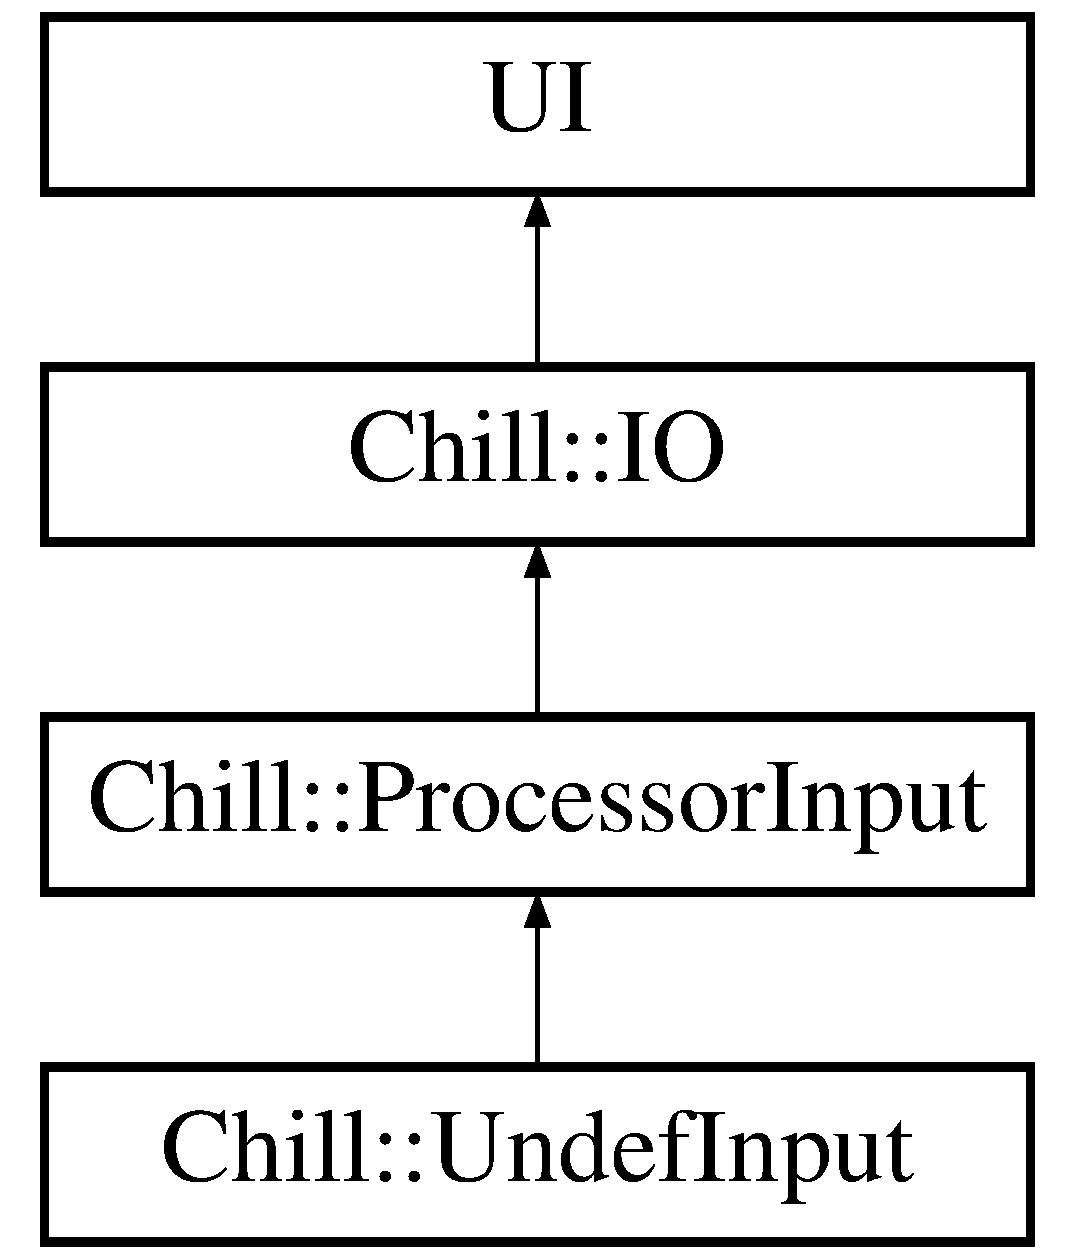
\includegraphics[height=4.000000cm]{class_chill_1_1_undef_input}
\end{center}
\end{figure}
\subsection*{Public Member Functions}
\begin{DoxyCompactItemize}
\item 
\mbox{\Hypertarget{class_chill_1_1_undef_input_a09536f796e0151b75d66114c1dc8960d}\label{class_chill_1_1_undef_input_a09536f796e0151b75d66114c1dc8960d}} 
bool {\bfseries draw\+Tweak} ()
\item 
\mbox{\Hypertarget{class_chill_1_1_undef_input_a066afdd58b9cc04b2b94375bc20c5209}\label{class_chill_1_1_undef_input_a066afdd58b9cc04b2b94375bc20c5209}} 
Auto\+Ptr$<$ \mbox{\hyperlink{class_chill_1_1_processor_input}{Processor\+Input}} $>$ {\bfseries clone} ()
\end{DoxyCompactItemize}
\subsection*{Additional Inherited Members}


The documentation for this class was generated from the following files\+:\begin{DoxyCompactItemize}
\item 
E\+:/\+Chill/chill/chill\+Engine/\mbox{\hyperlink{_i_os_8h}{I\+Os.\+h}}\item 
E\+:/\+Chill/chill/chill\+Engine/I\+Os.\+cpp\end{DoxyCompactItemize}

\hypertarget{class_chill_1_1_undef_output}{}\section{Chill\+:\+:Undef\+Output Class Reference}
\label{class_chill_1_1_undef_output}\index{Chill\+::\+Undef\+Output@{Chill\+::\+Undef\+Output}}
Inheritance diagram for Chill\+:\+:Undef\+Output\+:\begin{figure}[H]
\begin{center}
\leavevmode
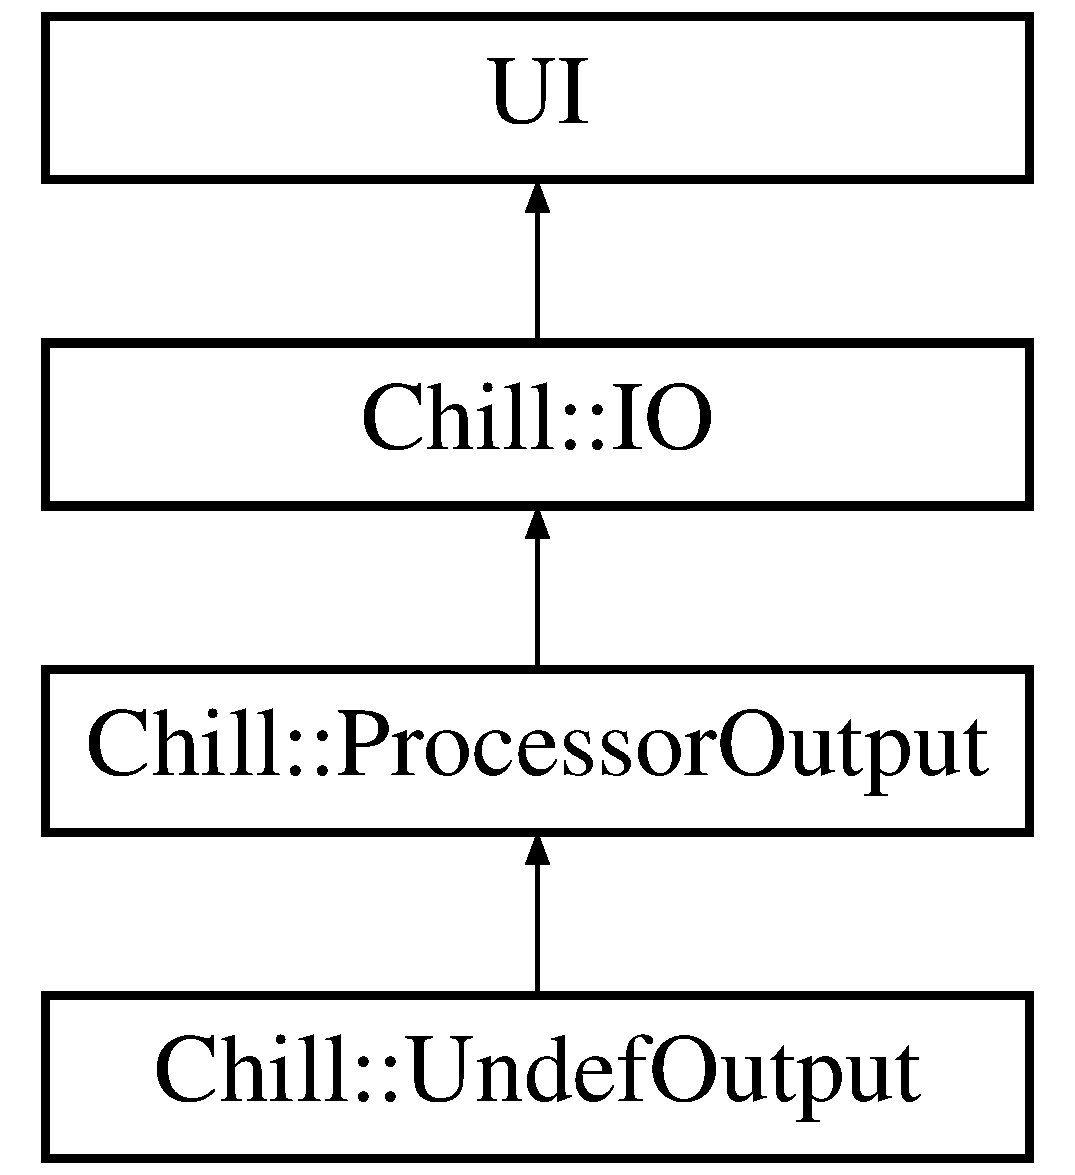
\includegraphics[height=4.000000cm]{class_chill_1_1_undef_output}
\end{center}
\end{figure}
\subsection*{Public Member Functions}
\begin{DoxyCompactItemize}
\item 
\mbox{\Hypertarget{class_chill_1_1_undef_output_a1a5d3bf924174e059b50784b4b6b163b}\label{class_chill_1_1_undef_output_a1a5d3bf924174e059b50784b4b6b163b}} 
Auto\+Ptr$<$ \mbox{\hyperlink{class_chill_1_1_processor_output}{Processor\+Output}} $>$ {\bfseries clone} ()
\end{DoxyCompactItemize}
\subsection*{Additional Inherited Members}


The documentation for this class was generated from the following file\+:\begin{DoxyCompactItemize}
\item 
E\+:/\+Chill/chill/chill\+Engine/\mbox{\hyperlink{_i_os_8h}{I\+Os.\+h}}\end{DoxyCompactItemize}

\hypertarget{class_chill_1_1_vec3_input}{}\section{Chill\+:\+:Vec3\+Input Class Reference}
\label{class_chill_1_1_vec3_input}\index{Chill\+::\+Vec3\+Input@{Chill\+::\+Vec3\+Input}}
Inheritance diagram for Chill\+:\+:Vec3\+Input\+:\begin{figure}[H]
\begin{center}
\leavevmode
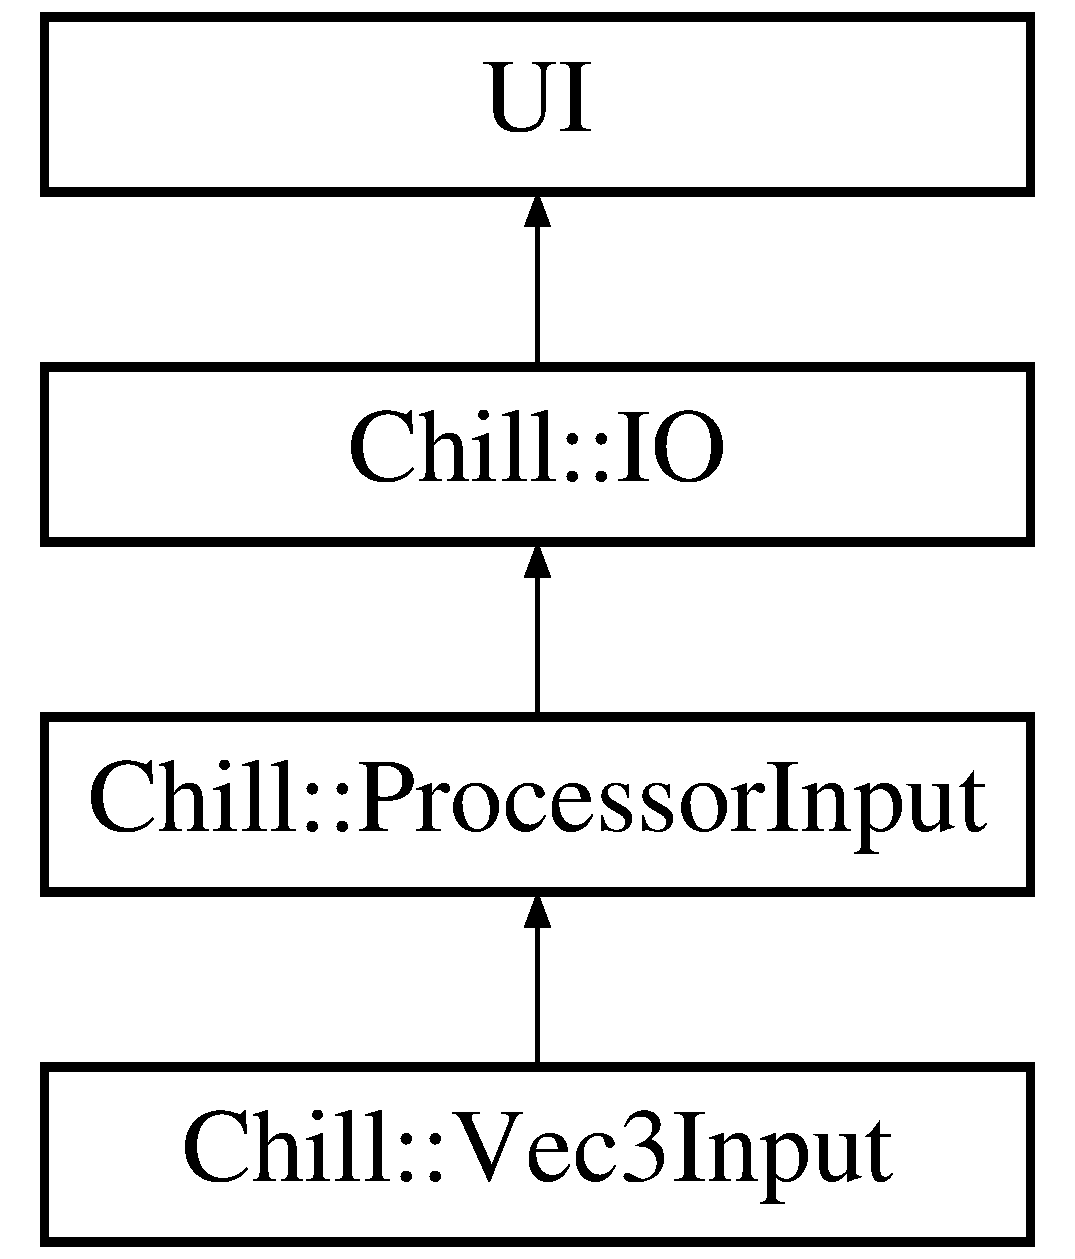
\includegraphics[height=4.000000cm]{class_chill_1_1_vec3_input}
\end{center}
\end{figure}
\subsection*{Public Member Functions}
\begin{DoxyCompactItemize}
\item 
\mbox{\Hypertarget{class_chill_1_1_vec3_input_a2340c3853f43091e59edcc2ce8f186dc}\label{class_chill_1_1_vec3_input_a2340c3853f43091e59edcc2ce8f186dc}} 
{\footnotesize template$<$typename ... Args$>$ }\\{\bfseries Vec3\+Input} (float \+\_\+value=0.\+0f, Args \&\&... \+\_\+args)
\item 
\mbox{\Hypertarget{class_chill_1_1_vec3_input_a7909e5998130ae3bf00838b6becfc3a7}\label{class_chill_1_1_vec3_input_a7909e5998130ae3bf00838b6becfc3a7}} 
{\footnotesize template$<$typename ... Args$>$ }\\{\bfseries Vec3\+Input} (float $\ast$\+\_\+value, float \+\_\+min=min(), float \+\_\+max=max(), float \+\_\+step=step(), Args \&\&...)
\item 
\mbox{\Hypertarget{class_chill_1_1_vec3_input_a9f4c1d5907e0f4f4625b94858586585f}\label{class_chill_1_1_vec3_input_a9f4c1d5907e0f4f4625b94858586585f}} 
bool {\bfseries draw\+Tweak} ()
\item 
\mbox{\Hypertarget{class_chill_1_1_vec3_input_a24d5f2814c131de79a49fdc71f2579d6}\label{class_chill_1_1_vec3_input_a24d5f2814c131de79a49fdc71f2579d6}} 
Auto\+Ptr$<$ \mbox{\hyperlink{class_chill_1_1_processor_input}{Processor\+Input}} $>$ {\bfseries clone} ()
\item 
\mbox{\Hypertarget{class_chill_1_1_vec3_input_ae37b296788799e66846d04d39cd89246}\label{class_chill_1_1_vec3_input_ae37b296788799e66846d04d39cd89246}} 
void {\bfseries save} (std\+::ofstream \&\+\_\+stream)
\end{DoxyCompactItemize}
\subsection*{Static Public Member Functions}
\begin{DoxyCompactItemize}
\item 
\mbox{\Hypertarget{class_chill_1_1_vec3_input_a998b4d13976407b3f0df952caa1d386f}\label{class_chill_1_1_vec3_input_a998b4d13976407b3f0df952caa1d386f}} 
static float {\bfseries min} ()
\item 
\mbox{\Hypertarget{class_chill_1_1_vec3_input_a66f0d41329891c8df5b36612e1c43441}\label{class_chill_1_1_vec3_input_a66f0d41329891c8df5b36612e1c43441}} 
static float {\bfseries max} ()
\item 
\mbox{\Hypertarget{class_chill_1_1_vec3_input_a3acbedadb55f3f59324145bf72373825}\label{class_chill_1_1_vec3_input_a3acbedadb55f3f59324145bf72373825}} 
static float {\bfseries step} ()
\end{DoxyCompactItemize}
\subsection*{Public Attributes}
\begin{DoxyCompactItemize}
\item 
\mbox{\Hypertarget{class_chill_1_1_vec3_input_a225abab9372f3b06d8704c13f4d8bc8a}\label{class_chill_1_1_vec3_input_a225abab9372f3b06d8704c13f4d8bc8a}} 
float {\bfseries m\+\_\+value} \mbox{[}3\mbox{]}
\item 
\mbox{\Hypertarget{class_chill_1_1_vec3_input_a368659db4d1a119212a199e3bf373ce4}\label{class_chill_1_1_vec3_input_a368659db4d1a119212a199e3bf373ce4}} 
float {\bfseries m\+\_\+min}
\item 
\mbox{\Hypertarget{class_chill_1_1_vec3_input_a8a587ebaba45b941bc6cc58143600b32}\label{class_chill_1_1_vec3_input_a8a587ebaba45b941bc6cc58143600b32}} 
float {\bfseries m\+\_\+max}
\item 
\mbox{\Hypertarget{class_chill_1_1_vec3_input_a37e78914224a0d3e9f3a3b3cac8e1730}\label{class_chill_1_1_vec3_input_a37e78914224a0d3e9f3a3b3cac8e1730}} 
float {\bfseries m\+\_\+step}
\end{DoxyCompactItemize}


The documentation for this class was generated from the following files\+:\begin{DoxyCompactItemize}
\item 
E\+:/\+Chill/chill/chill\+Engine/\mbox{\hyperlink{_i_os_8h}{I\+Os.\+h}}\item 
E\+:/\+Chill/chill/chill\+Engine/I\+Os.\+cpp\end{DoxyCompactItemize}

\hypertarget{class_chill_1_1_vec3_output}{}\section{Chill\+:\+:Vec3\+Output Class Reference}
\label{class_chill_1_1_vec3_output}\index{Chill\+::\+Vec3\+Output@{Chill\+::\+Vec3\+Output}}
Inheritance diagram for Chill\+:\+:Vec3\+Output\+:\begin{figure}[H]
\begin{center}
\leavevmode
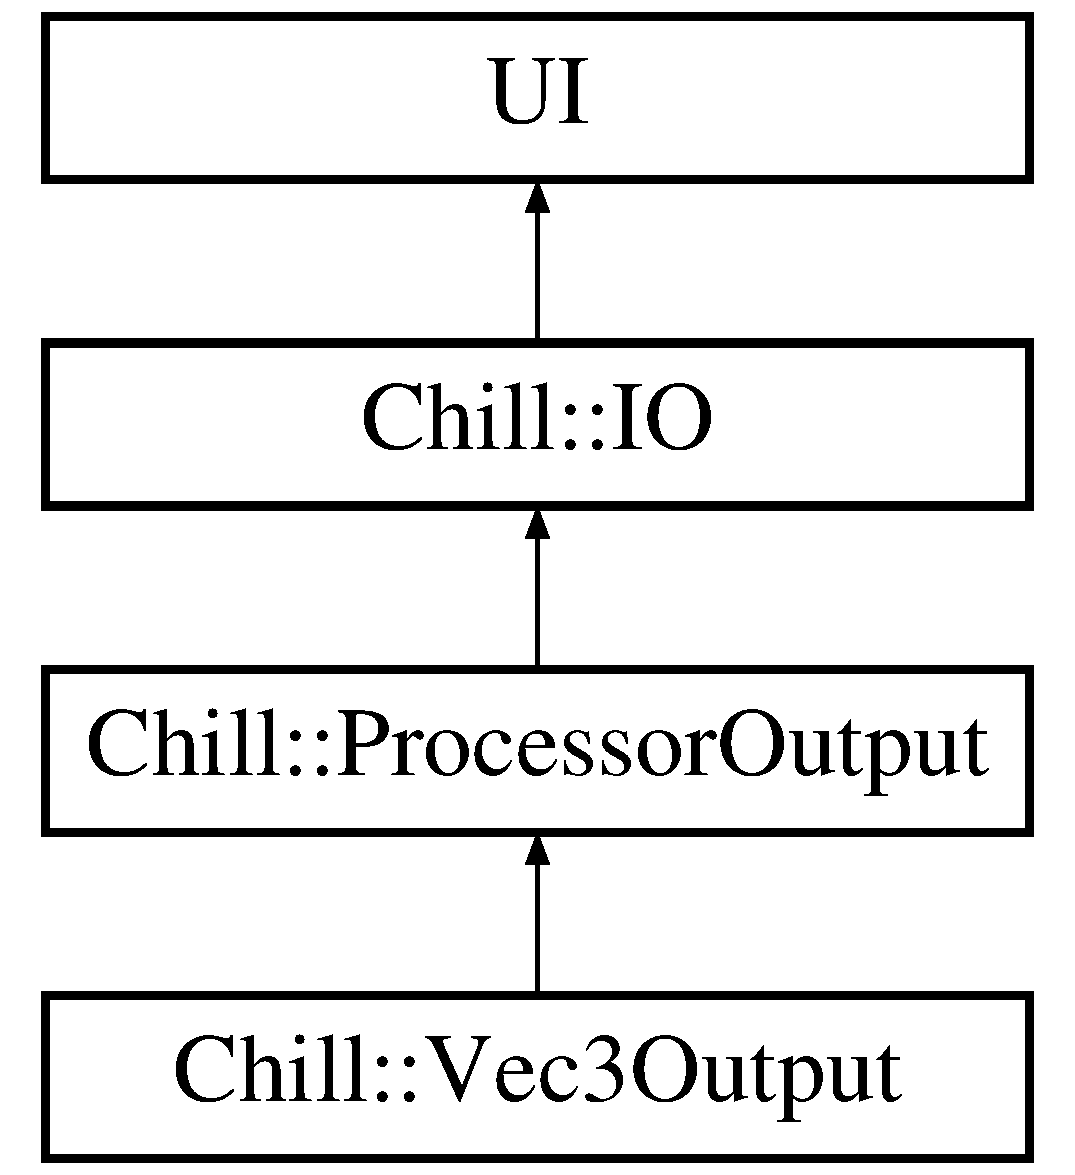
\includegraphics[height=4.000000cm]{class_chill_1_1_vec3_output}
\end{center}
\end{figure}
\subsection*{Public Member Functions}
\begin{DoxyCompactItemize}
\item 
\mbox{\Hypertarget{class_chill_1_1_vec3_output_a9a23ba7d29f8ea2d5704f892ce038ee8}\label{class_chill_1_1_vec3_output_a9a23ba7d29f8ea2d5704f892ce038ee8}} 
Auto\+Ptr$<$ \mbox{\hyperlink{class_chill_1_1_processor_output}{Processor\+Output}} $>$ {\bfseries clone} ()
\end{DoxyCompactItemize}
\subsection*{Additional Inherited Members}


The documentation for this class was generated from the following file\+:\begin{DoxyCompactItemize}
\item 
E\+:/\+Chill/chill/chill\+Engine/\mbox{\hyperlink{_i_os_8h}{I\+Os.\+h}}\end{DoxyCompactItemize}

\hypertarget{class_chill_1_1_vec4_input}{}\section{Chill\+:\+:Vec4\+Input Class Reference}
\label{class_chill_1_1_vec4_input}\index{Chill\+::\+Vec4\+Input@{Chill\+::\+Vec4\+Input}}
Inheritance diagram for Chill\+:\+:Vec4\+Input\+:\begin{figure}[H]
\begin{center}
\leavevmode
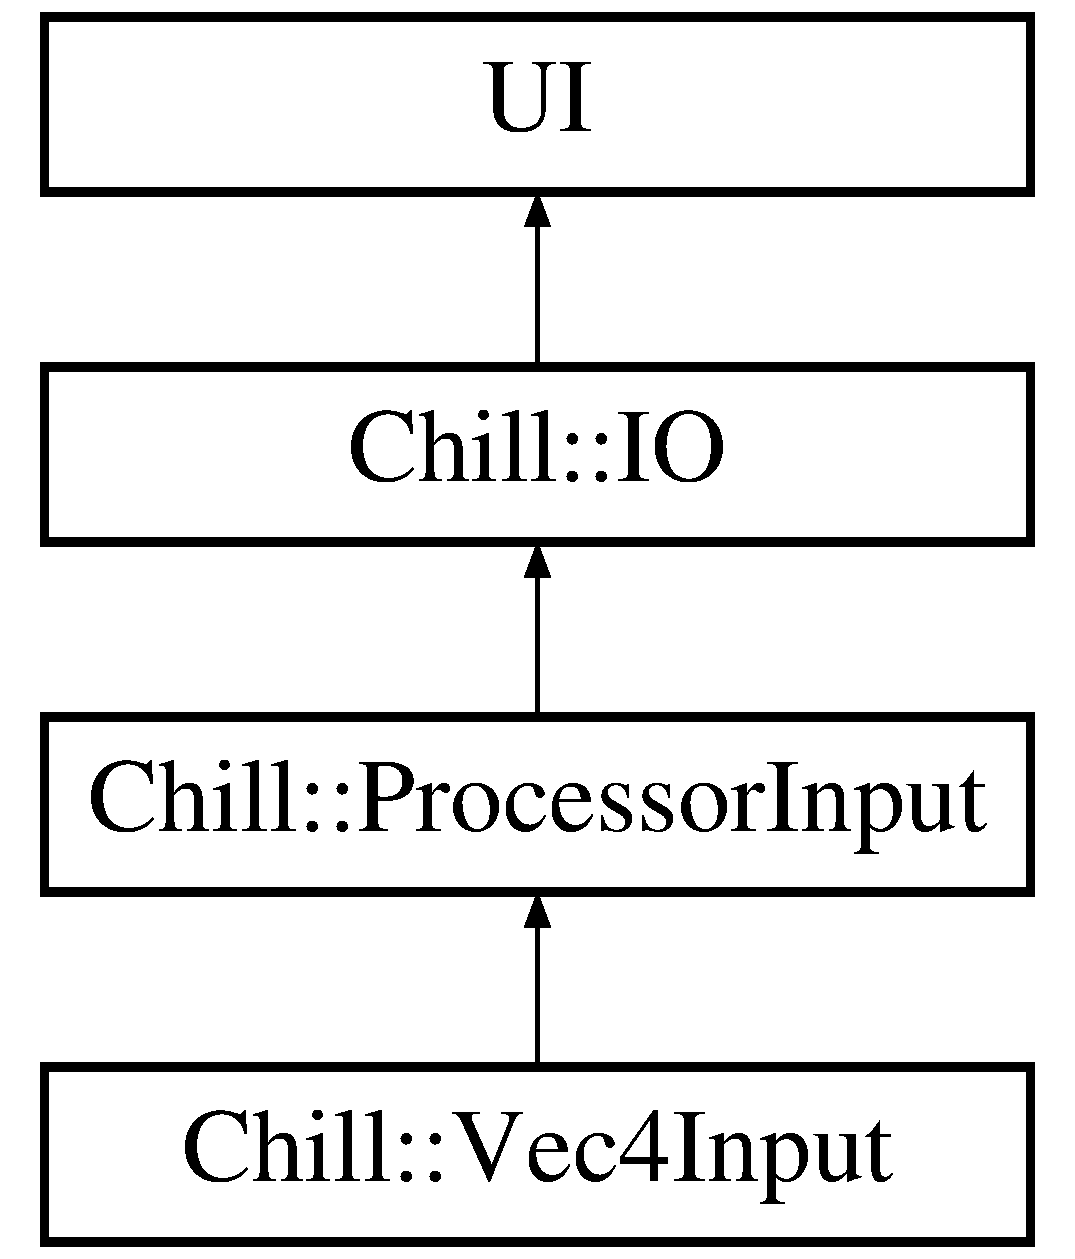
\includegraphics[height=4.000000cm]{class_chill_1_1_vec4_input}
\end{center}
\end{figure}
\subsection*{Public Member Functions}
\begin{DoxyCompactItemize}
\item 
\mbox{\Hypertarget{class_chill_1_1_vec4_input_a4742a9ad94a06707c683b0117a591ced}\label{class_chill_1_1_vec4_input_a4742a9ad94a06707c683b0117a591ced}} 
{\footnotesize template$<$typename ... Args$>$ }\\{\bfseries Vec4\+Input} (float \+\_\+value=0.\+0f, Args \&\&... \+\_\+args)
\item 
\mbox{\Hypertarget{class_chill_1_1_vec4_input_a1367befcccd20b51bb383f912156269d}\label{class_chill_1_1_vec4_input_a1367befcccd20b51bb383f912156269d}} 
{\footnotesize template$<$typename ... Args$>$ }\\{\bfseries Vec4\+Input} (float $\ast$\+\_\+value, float \+\_\+min=min(), float \+\_\+max=max(), bool \+\_\+picker=false, float \+\_\+step=step(), Args \&\&...)
\item 
\mbox{\Hypertarget{class_chill_1_1_vec4_input_a7b4a7489d7bd2a275a5b04ddd9c9d399}\label{class_chill_1_1_vec4_input_a7b4a7489d7bd2a275a5b04ddd9c9d399}} 
bool {\bfseries draw\+Tweak} ()
\item 
\mbox{\Hypertarget{class_chill_1_1_vec4_input_a5afbe983425e75d3859ea933c4d5fb1c}\label{class_chill_1_1_vec4_input_a5afbe983425e75d3859ea933c4d5fb1c}} 
Auto\+Ptr$<$ \mbox{\hyperlink{class_chill_1_1_processor_input}{Processor\+Input}} $>$ {\bfseries clone} ()
\item 
\mbox{\Hypertarget{class_chill_1_1_vec4_input_a35eb6775dd8794995129153ca8eda12b}\label{class_chill_1_1_vec4_input_a35eb6775dd8794995129153ca8eda12b}} 
void {\bfseries save} (std\+::ofstream \&\+\_\+stream)
\end{DoxyCompactItemize}
\subsection*{Static Public Member Functions}
\begin{DoxyCompactItemize}
\item 
\mbox{\Hypertarget{class_chill_1_1_vec4_input_a92f664df3bd480d29e3eb8dc97758fb3}\label{class_chill_1_1_vec4_input_a92f664df3bd480d29e3eb8dc97758fb3}} 
static float {\bfseries min} ()
\item 
\mbox{\Hypertarget{class_chill_1_1_vec4_input_ad810cc739c23584df693973da9262b19}\label{class_chill_1_1_vec4_input_ad810cc739c23584df693973da9262b19}} 
static float {\bfseries max} ()
\item 
\mbox{\Hypertarget{class_chill_1_1_vec4_input_a90702ff48623192730324b48eba0cc7f}\label{class_chill_1_1_vec4_input_a90702ff48623192730324b48eba0cc7f}} 
static float {\bfseries step} ()
\end{DoxyCompactItemize}
\subsection*{Public Attributes}
\begin{DoxyCompactItemize}
\item 
\mbox{\Hypertarget{class_chill_1_1_vec4_input_a66d187a72e0528509020a3d488ff653a}\label{class_chill_1_1_vec4_input_a66d187a72e0528509020a3d488ff653a}} 
float {\bfseries m\+\_\+value} \mbox{[}4\mbox{]}
\item 
\mbox{\Hypertarget{class_chill_1_1_vec4_input_a8957f9578b241426ccdd827a3dc1efef}\label{class_chill_1_1_vec4_input_a8957f9578b241426ccdd827a3dc1efef}} 
float {\bfseries m\+\_\+min}
\item 
\mbox{\Hypertarget{class_chill_1_1_vec4_input_a4a2b9e0dc8b7f502bb40b143d14bf88d}\label{class_chill_1_1_vec4_input_a4a2b9e0dc8b7f502bb40b143d14bf88d}} 
float {\bfseries m\+\_\+max}
\item 
\mbox{\Hypertarget{class_chill_1_1_vec4_input_ab0f331608a8c9a87bec813c98924aa9c}\label{class_chill_1_1_vec4_input_ab0f331608a8c9a87bec813c98924aa9c}} 
bool {\bfseries m\+\_\+colorpicker}
\item 
\mbox{\Hypertarget{class_chill_1_1_vec4_input_ad537a48553b5bc4b4edf69f9ecf4b3a1}\label{class_chill_1_1_vec4_input_ad537a48553b5bc4b4edf69f9ecf4b3a1}} 
float {\bfseries m\+\_\+step}
\end{DoxyCompactItemize}


The documentation for this class was generated from the following files\+:\begin{DoxyCompactItemize}
\item 
E\+:/\+Chill/chill/chill\+Engine/\mbox{\hyperlink{_i_os_8h}{I\+Os.\+h}}\item 
E\+:/\+Chill/chill/chill\+Engine/I\+Os.\+cpp\end{DoxyCompactItemize}

\hypertarget{class_chill_1_1_vec4_output}{}\section{Chill\+:\+:Vec4\+Output Class Reference}
\label{class_chill_1_1_vec4_output}\index{Chill\+::\+Vec4\+Output@{Chill\+::\+Vec4\+Output}}
Inheritance diagram for Chill\+:\+:Vec4\+Output\+:\begin{figure}[H]
\begin{center}
\leavevmode
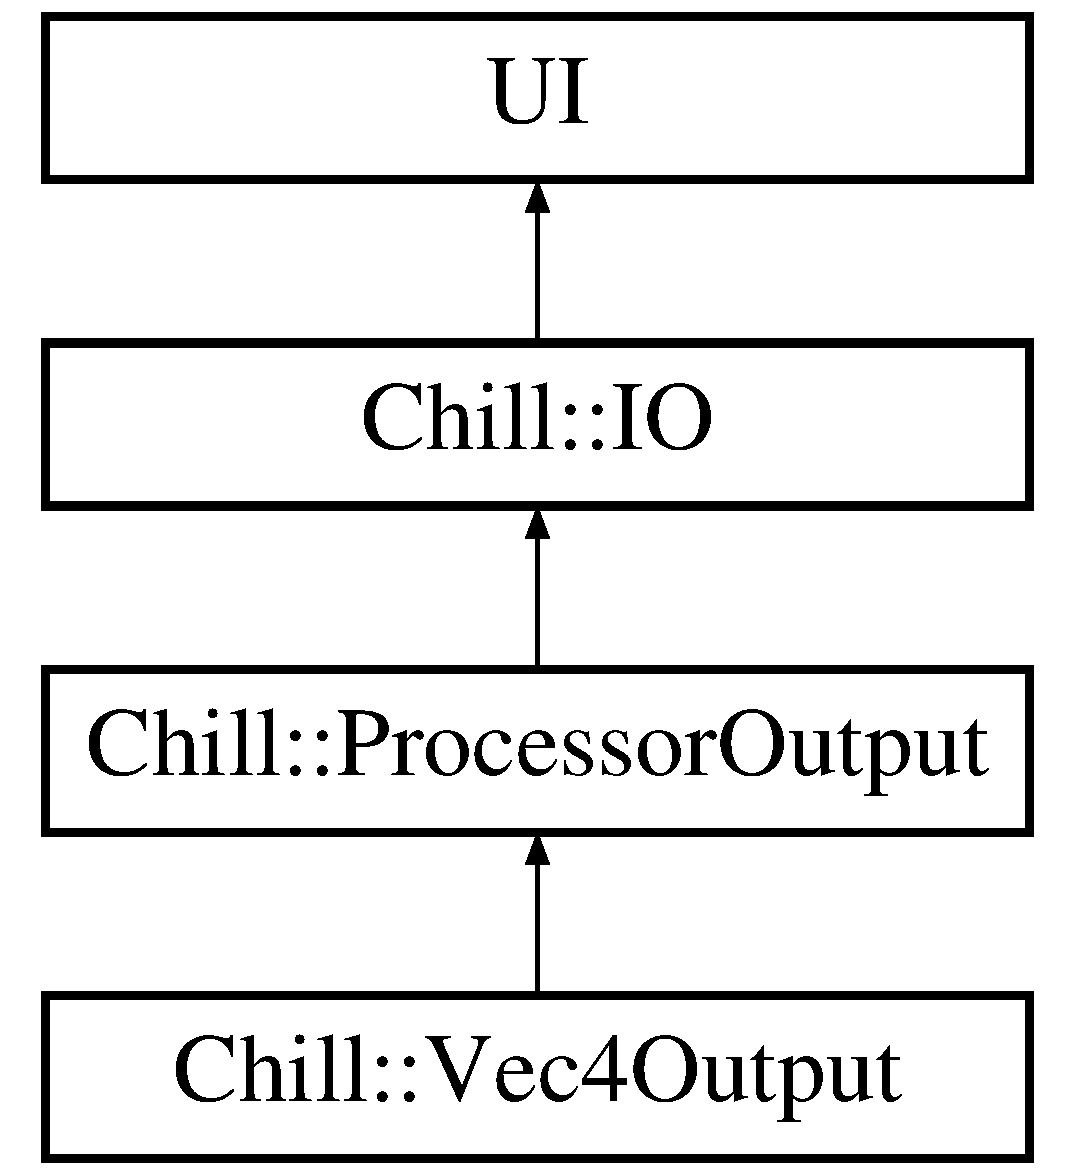
\includegraphics[height=4.000000cm]{class_chill_1_1_vec4_output}
\end{center}
\end{figure}
\subsection*{Public Member Functions}
\begin{DoxyCompactItemize}
\item 
\mbox{\Hypertarget{class_chill_1_1_vec4_output_afd45e3cdb874f7be8660aadfb8bbeb2d}\label{class_chill_1_1_vec4_output_afd45e3cdb874f7be8660aadfb8bbeb2d}} 
Auto\+Ptr$<$ \mbox{\hyperlink{class_chill_1_1_processor_output}{Processor\+Output}} $>$ {\bfseries clone} ()
\end{DoxyCompactItemize}
\subsection*{Additional Inherited Members}


The documentation for this class was generated from the following file\+:\begin{DoxyCompactItemize}
\item 
E\+:/\+Chill/chill/chill\+Engine/\mbox{\hyperlink{_i_os_8h}{I\+Os.\+h}}\end{DoxyCompactItemize}

\chapter{File Documentation}
\hypertarget{_i_os_8h}{}\section{E\+:/\+Chill/chill/chill\+Engine/\+I\+Os.h File Reference}
\label{_i_os_8h}\index{E\+:/\+Chill/chill/chill\+Engine/\+I\+Os.\+h@{E\+:/\+Chill/chill/chill\+Engine/\+I\+Os.\+h}}
{\ttfamily \#include \char`\"{}Processor.\+h\char`\"{}}\newline
{\ttfamily \#include \char`\"{}I\+O\+Types.\+h\char`\"{}}\newline
\subsection*{Classes}
\begin{DoxyCompactItemize}
\item 
class \mbox{\hyperlink{class_chill_1_1_i_o}{Chill\+::\+IO}}
\item 
class \mbox{\hyperlink{class_chill_1_1_processor_output}{Chill\+::\+Processor\+Output}}
\item 
class \mbox{\hyperlink{class_chill_1_1_processor_input}{Chill\+::\+Processor\+Input}}
\item 
class \mbox{\hyperlink{class_chill_1_1_undef_input}{Chill\+::\+Undef\+Input}}
\item 
class \mbox{\hyperlink{class_chill_1_1_undef_output}{Chill\+::\+Undef\+Output}}
\item 
class \mbox{\hyperlink{class_chill_1_1_bool_input}{Chill\+::\+Bool\+Input}}
\item 
class \mbox{\hyperlink{class_chill_1_1_bool_output}{Chill\+::\+Bool\+Output}}
\item 
class \mbox{\hyperlink{class_chill_1_1_int_input}{Chill\+::\+Int\+Input}}
\item 
class \mbox{\hyperlink{class_chill_1_1_int_output}{Chill\+::\+Int\+Output}}
\item 
class \mbox{\hyperlink{class_chill_1_1_scalar_input}{Chill\+::\+Scalar\+Input}}
\item 
class \mbox{\hyperlink{class_chill_1_1_scalar_output}{Chill\+::\+Scalar\+Output}}
\item 
class \mbox{\hyperlink{class_chill_1_1_shape_input}{Chill\+::\+Shape\+Input}}
\item 
class \mbox{\hyperlink{class_chill_1_1_shape_output}{Chill\+::\+Shape\+Output}}
\item 
class \mbox{\hyperlink{class_chill_1_1_vec4_input}{Chill\+::\+Vec4\+Input}}
\item 
class \mbox{\hyperlink{class_chill_1_1_vec4_output}{Chill\+::\+Vec4\+Output}}
\item 
class \mbox{\hyperlink{class_chill_1_1_vec3_input}{Chill\+::\+Vec3\+Input}}
\item 
class \mbox{\hyperlink{class_chill_1_1_vec3_output}{Chill\+::\+Vec3\+Output}}
\end{DoxyCompactItemize}

\hypertarget{_processing_graph_8h}{}\section{E\+:/\+Chill/chill/chill\+Engine/\+Processing\+Graph.h File Reference}
\label{_processing_graph_8h}\index{E\+:/\+Chill/chill/chill\+Engine/\+Processing\+Graph.\+h@{E\+:/\+Chill/chill/chill\+Engine/\+Processing\+Graph.\+h}}
{\ttfamily \#include $<$vector$>$}\newline
{\ttfamily \#include $<$Lib\+S\+L.\+h$>$}\newline
{\ttfamily \#include \char`\"{}Processor.\+h\char`\"{}}\newline
\subsection*{Classes}
\begin{DoxyCompactItemize}
\item 
class \mbox{\hyperlink{class_chill_1_1_processing_graph}{Chill\+::\+Processing\+Graph}}
\end{DoxyCompactItemize}

\hypertarget{_processor_8h}{}\section{E\+:/\+Chill/chill/chill\+Engine/\+Processor.h File Reference}
\label{_processor_8h}\index{E\+:/\+Chill/chill/chill\+Engine/\+Processor.\+h@{E\+:/\+Chill/chill/chill\+Engine/\+Processor.\+h}}
{\ttfamily \#include $<$Lib\+S\+L.\+h$>$}\newline
{\ttfamily \#include \char`\"{}U\+I.\+h\char`\"{}}\newline
{\ttfamily \#include \char`\"{}I\+O\+Types.\+h\char`\"{}}\newline
{\ttfamily \#include \char`\"{}I\+Os.\+h\char`\"{}}\newline
\subsection*{Classes}
\begin{DoxyCompactItemize}
\item 
class \mbox{\hyperlink{class_chill_1_1_processor}{Chill\+::\+Processor}}
\item 
class \mbox{\hyperlink{class_chill_1_1_lua_processor}{Chill\+::\+Lua\+Processor}}
\item 
class \mbox{\hyperlink{class_chill_1_1_group_processor}{Chill\+::\+Group\+Processor}}
\item 
class \mbox{\hyperlink{class_chill_1_1_multiplexer}{Chill\+::\+Multiplexer}}
\end{DoxyCompactItemize}

%--- End generated contents ---

% Index
\backmatter
\newpage
\phantomsection
\clearemptydoublepage
\addcontentsline{toc}{chapter}{Index}
\printindex

\end{document}
